\documentclass[conference]{IEEEtran}
\IEEEoverridecommandlockouts
% The preceding line is only needed to identify funding in the first footnote. If that is unneeded, please comment it out.
\usepackage{cite}
\usepackage{amsmath,amssymb,amsfonts}
\usepackage{graphicx}
\usepackage{textcomp}
\usepackage{xcolor}
\usepackage{multirow}
\usepackage{tabularx}
\usepackage{booktabs}
\usepackage{stfloats}
\usepackage{subcaption}
\usepackage{float}
\usepackage{placeins}
\usepackage{listings}
\usepackage[ruled,vlined,linesnumbered]{algorithm2e}
% JavaScript language definition for listings
\lstdefinelanguage{JavaScript}{
  keywords={const,let,var,function,return,if,else,for,while,do,switch,case,break,
             continue,new,delete,typeof,instanceof,in,of,async,await,class,extends,
             import,export,default,try,catch,finally,throw,true,false,null,undefined},
  keywordstyle=\color{blue}\bfseries,
  ndkeywords={z,enum,string,optional},
  ndkeywordstyle=\color{purple}\bfseries,
  sensitive=true,
  comment=[l]{//},
  morecomment=[s]{/*}{*/},
  commentstyle=\color{gray}\itshape,
  stringstyle=\color{orange},
  morestring=[b]",
  morestring=[b]'
}
\lstset{
  basicstyle=\ttfamily\footnotesize,
  breaklines=true,
  frame=single,
  language=JavaScript,
  showstringspaces=false
}

\def\BibTeX{{\rm B\kern-.05em{\sc i\kern-.025em b}\kern-.08em
    T\kern-.1667em\lower.7ex\hbox{E}\kern-.125emX}}
\begin{document}

\title{
AI Agent Orchestrated Phishing Detection Using Natural Language Processing and Machine Learning\\
}

\author{
\IEEEauthorblockN{Tolga Üner}
\IEEEauthorblockA{
\textit{Computer Engineering Dept.} \\
\textit{Dokuz Eylul University
} \\
İzmir, Türkiye \\
tolga.uner@ogr.deu.edu.tr
}

\and

\IEEEauthorblockN{Gökhan Dalkılıç }
\IEEEauthorblockA{
\textit{Computer Engineering Dept.} \\
\textit{Dokuz Eylul University
} \\
İzmir, Türkiye \\
gokhan.dalkilic@deu.edu.tr
}
}

\maketitle



\begin{abstract}
This document is a model and instructions for \LaTeX.
This and the IEEEtran.cls file define the components of your paper [title, text, heads, etc.]. *CRITICAL: Do Not Use Symbols, Special Characters, Footnotes,
or Math in Paper Title or Abstract.
\end{abstract}

\begin{IEEEkeywords}

Phishing Detection, Text Analysis, Machine Learning Methods, Deep Neural Networks, Model Context Protocol, Cybersecurity, AI Agent

\end{IEEEkeywords}

\section{Introduction}
This document is a model and instructions for \LaTeX.Please observe the conference page limits.

\section{Related Works}

Paradkar explored which machine learning and deep learning methods are best for detecting Phishing Emails. This study uses the ENRON Corpus, which has over 500,000 emails. The research utilized a sample of 20,000 emails, of which 8,336 were phishing, and 11,664 were verified as safe. After that, the data was preprocessed, and then the study evaluated models categorized into machine learning classifiers, such as Logistic Regression, Naive Bayes, SVM, and Decision Trees, and deep learning architectures, including CNN, LSTM, and Bidirectional-LSTM. The machine learning techniques gave worse results than the deep learning techniques \cite{paradkar2023phishing}.

Alhogail and  Alsabih investigated detecting phishing emails using machine learning and Natural Language Processing. To detect phishing emails the study goes through three phases. The first phase is collecting data and preparing it for training and testing. This study used a fraud dataset that is available to the public. Normal emails are labeled as 0, and phishing emails are labeled as 1. The dataset contains 3685 phishing emails and 4894 normal emails. After preparing the data they created a deep learning GCN algorithm and fed the data to the classifier, and prepared for evaluation. The final part is to test the data to validate the model. As a result, the created model gave an accuracy of 98.2\%, and the precision of 98.5\% \cite{alhogail2021applying}.


Egozi explained that phishing emails are still a big problem. To solve the problem, the authors came up with a model that had new features. The two steps of the proposed model are machine learning and feature extraction. The model uses 26 features to figure out if the emails are phishing or legitimate (ham). Different machine learning models work best with different sets of data. The study tried out 17 models, and 14 of them worked well. The authors utilized data from the IWSPA competition for the dataset. The training dataset contains 735 phishing emails and 3865 ham emails. The testing dataset contains 475 phishing emails and 3824 ham emails. The detector successfully identified 95\% of legitimate emails and 80\% of phishing attempts \cite{egozi2018phishing}.


Anirudh explored ways to improve detecting phishing mail by combining Support Vector Machine (SVM), XGBoost algorithms, and logistic regression to create a better system. These algorithms do independent analyses of the data and make their own predictions. The combination layer then compiles these forecasts. The combination of these predictions is then used to train a meta learner. It learns how to use these predictions most effectively by figuring out the appropriate weights for them throughout the training process. The dataset has 18650 emails. All of them are tagged either "Safe Email" or "Phishing Email". As a result 11322 emails are tagged "Safe Email" and the remaining 7328 emails are tagged "Phishing Email". SVM, Random Forest, Multinomial-Naïve Bayes, and XGBoost algorithms were used to compare the outcomes of the suggested methodology in order to evaluate its effectiveness. Multinomial Naive Bayes (MNB) had an accuracy of 96.22, a precision score of 96.36, and a recall score of 97.36.  and an overall F1-score of 96.96. SVM had an accuracy of 96.74\%, a precision score of 98.05\%, a recall score of 96.52\%, and an overall F1-score of 97.28\%. XGBoost had an accuracy of 96.05\%, a precision score of 97.75\%, a recall score of 95.67\%, and an overall F1-score of 96.70\%. Random Forest had an accuracy of 97.06\%, a precision score of 97.92\%, a recall score of 97.33\%, and an overall F1-score of 97.62\%. The accuracy of the proposed method is 97.92\%, surpassing the performance of other models. The proposed method had a precision score of 98.43\%, a recall of 98.22\%, and a 98.32\% overall F1-score \cite{anirudh2024ensemble}.

Chinta et al. proposed a mixed model that uses both BERT and LSTM to detect phishing emails. The study uses preprocessing steps like tokenization, stemming, and getting rid of HTML tags, stop words, and punctuation to get the email content ready. Using methods like TF-IDF, features are taken out and turned into numerical vectors that ML models can use. The suggested BERT-LSTM model uses BERT to understand context and LSTM to find patterns in sequences. This solves problems like vanishing gradients in RNNs. When put to the test, the model was much better than baseline models like Naïve Bayes, RNN, and SVM, getting 99.55\% accuracy and a 99.24 F1-score. Despite high performance, the model needs a lot of labeled data and a lot of computing power, which could make it hard to use in real life \cite{chinta2025building}.


 Bountakas et al. investigated the effectiveness of different NLP and ML combinations by using only email body data for phishing detection. The research evaluates three NLP techniques, BERT, Word2Vec, and TF-IDF, for feature extraction, followed by classification using common ML algorithms such as Random Forest (RF), Logistic Regression (LR), Gradient Boosted Trees (GBT), and Decision Trees (DT). Two datasets were constructed: one balanced and one imbalanced (with a 1:10 phishing-to-benign email ratio), using the Enron corpus for benign emails and the Nazario phishing dataset.
The results show that Word2Vec did better than both TF-IDF and BERT on both datasets. Word2Vec with RF and LR got more than 95\% accuracy on the balanced dataset, while BERT-based models always did worse. Word2Vec with LR got the highest F1 score of 92.41\% on the imbalanced dataset, but BERT-based combinations got much lower scores. For example, LR + BERT only got 63.92\% F1 score.  \cite{bountakas2021comparison}.


Kumar et al. examined the performance of diverse machine learning classifiers in identifying spam emails, utilizing datasets from Kaggle and additional sources. The main dataset has 5,573 email samples, which are divided into two groups: 70\% for training and 30\% for testing.  Using the Scikit-learn framework with different experimental settings, the authors test eight classifiers: Random Forest, Decision Tree, K-Nearest Neighbor (KNN), Naïve Bayes, Support Vector Machine (SVM), AdaBoost, and Bagging.
The results show that Naive Bayes achieves the best individual scores up to 0.98 in precision and recall when parameters are adjusted and improved. On the other hand, AdaBoost and Bagging classifiers always get good scores across all metrics, around 0.94--0.95. Naïve Bayes works best in this study, but it has a flaw: it assumes that features are independent, which could make it less reliable in the real world. By combining several classifiers, ensemble methods help reduce variance and overfitting \cite{kumar2020email}.


Patil et al. used both Natural Language Processing (NLP) and machine learning algorithms to find phishing emails with a high level of accuracy.  There are three main steps in their method: preprocessing the text, extracting features, and supervised classification. Tokenization, normalization, and getting rid of irrelevant text elements are all standard NLP tasks that happen during the preprocessing stage. This makes it possible to extract discriminative linguistic features from email content. Feature representations are primarily based on statistical text representation methods, such as TF-IDF, which are then used as inputs for machine learning classifiers. To increase the performance of classification, the study applies ensemble learning strategies, specifically Stacking and Majority Voting, by combining multiple machine learning classifiers rather than relying on a single model. When using a labeled dataset of phishing and real emails, ensemble-based methods get better accuracy and F1-scores than single classifiers. The study is based on a large set of public phishing emails that includes more than 80,000 email records from a variety of publicly available sources. The dataset contains both phishing and legitimate emails and is similar in size, variety, and label distribution to Kaggle phishing email datasets that are widely used. The findings show that the combination of NLP-based feature extraction and ensemble learning enhances the reliability of phishing email detection. The Stacking ensemble method works the best of all the ones that were tested. It has an accuracy of 98.89\% and very low false positive and false negative rates of 0.01. But these performance improvements come at the cost of more complicated calculations, since ensemble models need to be trained for much longer periods of time, more than 2000 seconds \cite{patil2025integrating}.


\begin{table*}[!t]
\centering
\caption{Comparative Analysis of Related Works in Phishing Detection}
\label{tab:literature_review}
\small
\begin{tabularx}{\textwidth}{@{}l c l l X l l@{}}
\toprule
\textbf{Study} & \textbf{Year} & \textbf{Model} & \textbf{Dataset} & \textbf{NLP / Features} & \textbf{Metrics} & \textbf{Key Results} \\ \midrule
\cite{paradkar2023phishing} & 2023 & ML + DL & Enron & Tokenization, Padding & Acc, F1 & Acc: $\sim$98\% \\ \addlinespace
\cite{alhogail2021applying} & 2021 & GCN \& DL & CLAIR (8.5k) & PMI, TF-IDF, Graph & Acc, F1, FPR & Acc: 98.2\% \\ \addlinespace
\cite{egozi2018phishing} & 2018 & ML Ensemble & IWSPA & Word count, Punctuation & TPR & TPR: 83\% \\ \addlinespace
\cite{anirudh2024ensemble} & 2024 & Stacking (SVM, XGBoost) & Kaggle (18.6k) & TF-IDF, Stemming & Acc, F1 & Acc: 97.92\% \\ \addlinespace
\cite{chinta2025building} & 2025 & BERT-LSTM & Hybrid (Spam Assassin, UCI) & BERT, Self-attention & Acc, F1 & Acc: 99.55\% \\ \addlinespace
\cite{bountakas2021comparison} & 2021 & ML + NLP & Enron \& Nazario & Lemmatization, Chi-Sq & Acc, AUC & Acc: 98.95\%  \\ \addlinespace
\cite{kumar2020email} & 2020 & NB, SVC, KNN & Kaggle Spam & BOW, Stemming & Acc & Acc: 98\% \\ \addlinespace
\cite{patil2025integrating} & 2025 & Ensemble & Kaggle (82k) & TF-IDF, CountVect & Acc, F1 & Acc: 98.89\%  \\ \addlinespace
\textbf{Our Study} & \textbf{2026} & \textbf{Agentic MCP} & \textbf{Dual (18.6k/82.5k)} & \textbf{Hybrid TF-IDF + DL} & \textbf{Acc, Rec, F1} & \textbf{Acc: 98.90\% / Rec: 98.99\%} \\
\bottomrule
\end{tabularx}
\end{table*}



\section{SYSTEM ARCHITECTURE AND DESIGN}
\label{sec:architecture}

This chapter details the design and engineering of the proposed phishing detection system. The framework integrates an LLM-based AI Agent, a Model Context Protocol (MCP) server, and a Python execution backend. Together, these components form an automated pipeline capable of data cleaning, feature extraction, model training, performance evaluation, and self-healing error recovery.

\subsection{Overall System Architecture}
The system adopts a modular client-server paradigm centered around the Model Context Protocol (MCP). As illustrated in Figure~\ref{fig:sys_arch}, the framework comprises three core layers:

\begin{enumerate}
    \item \textbf{AI Agent Layer (Gemini Flash):} Functions as the central controller. It interprets experimental objectives, generates pipeline execution code, diagnoses runtime failures, and evaluates classification outputs.

    \item \textbf{MCP Server Layer (Node.js / Express):} Built on \texttt{server.js}, this layer exposes standardized tool interfaces validated via Zod schemas. It receives JSON-RPC requests from the agent, manages execution state using \texttt{run\_state.json}, and dispatches jobs to the Python environment.

    \item \textbf{Python Execution Engine (Backend):} Executes the machine learning and deep learning workloads, feature extraction scripts, and the \texttt{resource\_monitor.py} subsystem.
\end{enumerate}

\begin{figure}[htbp]
\centering
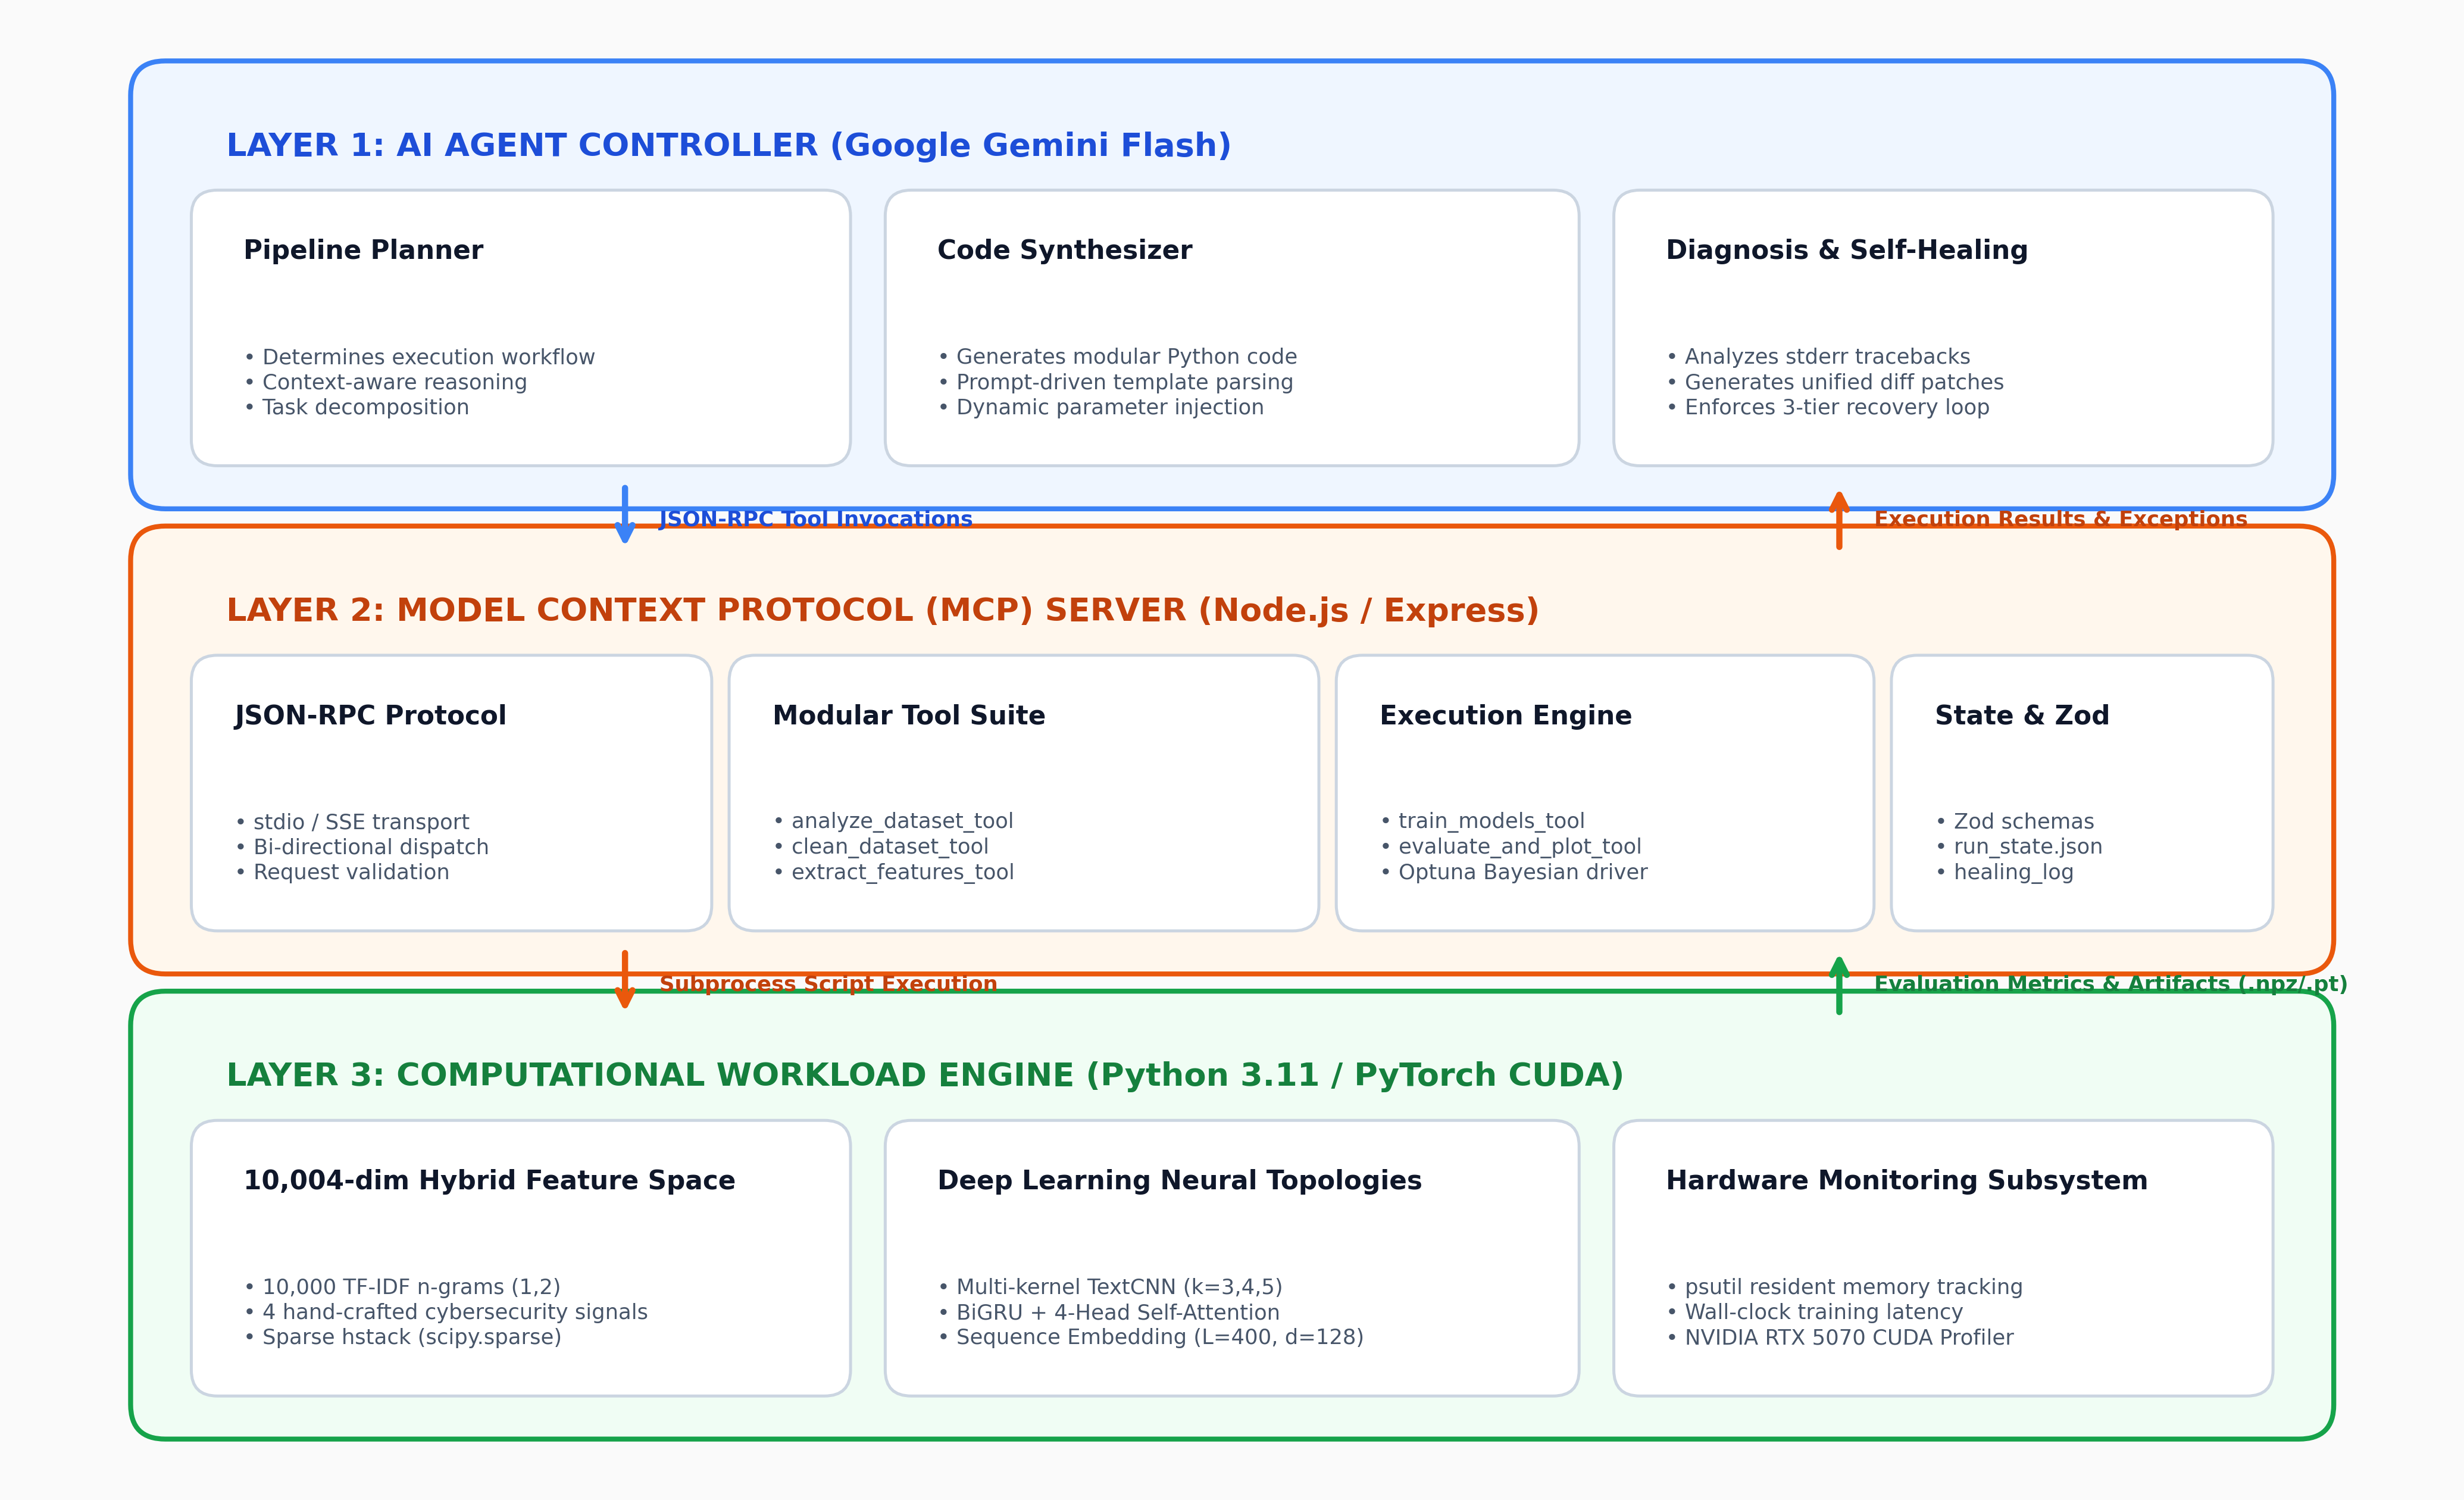
\includegraphics[width=\columnwidth]{ml-images-82/architecture_diagram.png}
\caption{Overall MCP-Based 3-Layer System Architecture: AI Agent (Gemini Flash), MCP Server (Node.js), and Python Computational Engine.}
\label{fig:sys_arch}
\end{figure}

\subsection{Model Context Protocol (MCP) in Detail}
The Model Context Protocol (MCP) is an open standard designed to structure interactions between large language models and external tool environments over standard input/output (\texttt{stdio}) channels.

\subsubsection{Technical Mechanics and Zod Validation}
Rather than invoking unconstrained command-line calls, the AI Agent communicates with execution tools defined on the MCP server. Each tool explicitly enforces an input parameter schema using Zod validation. For example, parameters such as dataset paths, model types, or feature limits are strictly validated prior to script execution:

\begin{lstlisting}[language=JavaScript, caption={Zod Schema Validation for Modular Training Tool}]
server.tool(
  "train_models_tool",
  "Train and Tune ML/DL Models",
  {
    mode: z.enum(["ML", "DL"]).default("ML"),
    features_npy_path: z.string(),
    labels_npy_path: z.string(),
    best_params_path: z.string().optional()
  },
  async (params) => { /* Subprocess Execution Logic */ }
);
\end{lstlisting}

This validation layer prevents malformed arguments from reaching the Python backend, ensuring reliable execution during autonomous pipeline loops.

\subsection{The AI Agent: Gemini Flash}
The orchestration agent is driven by Google's Gemini Flash model, selected for its rapid inference latency, structured JSON output capabilities, and native support for tool invocation.

\subsubsection{Agent Roles and Prompt Engineering Strategy}
The agent executes three distinct operational roles during an experiment run:
\begin{itemize}
    \item \textbf{Pipeline Planning:} Determines the sequence of execution (preprocessing $\rightarrow$ feature extraction $\rightarrow$ model training $\rightarrow$ evaluation).
    \item \textbf{Code Generation:} Synthesizes Python execution scripts based on modular prompt instructions (e.g., \texttt{train\_prompt.md}, \texttt{train\_dl\_prompt.md}).
    \item \textbf{Error Diagnosis:} Inspects stack trace logs when execution fails and devises corrective strategies.
\end{itemize}

State persistence is maintained through a structured memory file, \texttt{run\_state.json}. At each pipeline stage, completed steps, dataset statistics, and intermediate metrics are recorded, allowing the agent to resume execution without repeating earlier computational steps.

\subsection{The Self-Healing Mechanism}
A critical requirement for autonomous pipeline execution is resilience against runtime exceptions. During script execution, errors such as tensor dimension mismatches, missing dependencies, or syntax anomalies can halt the experiment. To prevent pipeline breakdown, we implement a three-tiered self-healing execution loop.

\subsubsection{Three-Tiered Recovery Workflow}
The recovery process operates sequentially across three levels:

\begin{enumerate}
    \item \textbf{Level 1 — Unified Patch Mode:} When an exception occurs, the error traceback and the broken script content are provided to the LLM. The agent generates a minimal unified \texttt{diff} patch. This patch is applied directly to the file using standard system patch utilities, avoiding a full code rewrite.

    \item \textbf{Level 2 — Full Rewrite Mode:} If the applied patch fails to resolve the crash on the second run, the agent performs a complete refactoring of the target script based on the updated error log.

    \item \textbf{Level 3 — Graceful Fallback and Prompt Refinement:} If errors persist after three attempts, execution halts safely. Diagnostic state is saved, allowing the researcher to refine the corresponding prompt template (\texttt{.md}) or adjust the execution environment manually.
\end{enumerate}

\begin{algorithm}[t]
\SetAlgoLined
\KwData{script\_path, python\_cmd, max\_attempts $= 3$}
\KwResult{Execution Output or Safe Exit}
attempt $\leftarrow$ 1\;
\While{attempt $\leq$ max\_attempts}{
  \eIf{executeScript(script\_path) succeeds}{
    \Return output\tcp*{Execution successful}
  }{
    \uIf{attempt $= 1$}{
      patch $\leftarrow$ generateUnifiedPatch(script\_path, error)\;
      applyPatch(script\_path, patch)\;
    }
    \uElseIf{attempt $= 2$}{
      new\_code $\leftarrow$ generateFullRewrite(script\_path, error)\;
      overwriteFile(script\_path, new\_code)\;
    }
    \Else{
      logSafeExit(script\_path, error)\;
      \Return{Execution Failed --- Manual Review Required}\;
    }
  }
  attempt $\leftarrow$ attempt $+ 1$\;
}
\caption{Multi-Tiered Self-Healing Script Execution Loop}
\label{alg:self_healing}
\end{algorithm}

All self-healing interventions, patch diffs, and execution attempts are persistently logged to \texttt{healing\_log.jsonl} to maintain an immutable audit trail of autonomous agent recovery actions.

\subsection{Tool Definitions}
The MCP Server defines five primary tools that constitute the operational surface for the AI Agent:

\begin{table}[htbp]
\caption{Summary of MCP Server Modular Tool Interfaces.}
\label{tab:mcp_tools}
\centering
\resizebox{\columnwidth}{!}{%
\begin{tabular}{@{}l p{4.2cm} p{3.2cm}@{}}
\toprule
\textbf{Tool Name} & \textbf{Key Responsibilities} & \textbf{Output Artifacts} \\ \midrule
\texttt{analyze\_dataset\_tool}   & Exploratory data analysis, missing value detection & \texttt{eda\_summary.json} \\ \addlinespace[2pt]
\texttt{clean\_dataset\_tool}     & Regex HTML/URL cleansing, metadata extraction      & \texttt{cleaned\_dataset.csv} \\ \addlinespace[2pt]
\texttt{extract\_features\_tool}  & Hybrid TF-IDF + Metadata / Subword tokenization    & \texttt{X\_train}, \texttt{y\_train} (.npy/.npz) \\ \addlinespace[2pt]
\texttt{train\_models\_tool}      & Optuna tuning, ML/DL model fitting, \texttt{auto\_model} & Trained model weights (.pt/.pkl) \\ \addlinespace[2pt]
\texttt{evaluate\_and\_plot\_tool}& ROC, CM, t-SNE, SHAP, calibration curves           & Performance JSON \& PNG plots \\ 
\bottomrule
\end{tabular}%
}
\end{table}

\subsection{Operational Data Flow}
The end-to-end execution follows a standardized sequence managed by JSON-based message passing:

\begin{enumerate}
    \item \textbf{Initialization:} The agent reads \texttt{run\_state.json} to verify previous step completions.
    \item \textbf{Data Cleaning:} The server invokes text preprocessing scripts; cleaned data is stored as CSV.
    \item \textbf{Feature Extraction:} Features are generated and serialized (\texttt{.npz} for ML matrices, \texttt{.npy} for DL sequence arrays).
    \item \textbf{Model Training \& Tuning:} Training tools execute hyperparameter searches across target model families.
    \item \textbf{Evaluation \& Visualization:} Performance metrics and figures (Confusion Matrices, ROC curves) are saved to structured output directories.
    \item \textbf{Standardized Response:} Final evaluation JSON arrays are returned to the agent context for reporting.
\end{enumerate}

\subsection{Resource Monitoring Subsystem}
To provide a multi-dimensional performance comparison between classical machine learning algorithms and deep neural networks, we incorporate a dedicated monitoring module (\texttt{resource\_monitor.py}).

Evaluating classification models strictly on accuracy metrics overlooks operational trade-offs such as computational overhead, memory footprints, and execution latency. The resource monitoring subsystem runs asynchronously alongside model training loops:

\begin{itemize}
    \item \textbf{Memory Tracking (RAM in MB):} Measures baseline memory before execution and tracks peak RSS (Resident Set Size) memory consumption during training using the \texttt{psutil} library.
    \item \textbf{Processor Utilization (CPU \%):} Samples CPU utilization at 100ms intervals across active execution threads.
    \item \textbf{Wall-Clock Execution Time (Seconds):} Measures exact elapsed time from data loading to model serialization.
\end{itemize}

These hardware metrics are recorded in each model's final evaluation JSON, enabling direct trade-off analysis between light-weight linear classifiers and complex deep learning topologies.

\subsection{Configuration and Computational Environment}
To ensure rigorous reproducibility of our autonomous experimental pipelines, the underlying hardware architecture and full-stack software dependencies are formally documented in Table~\ref{tab:system_env}.

\begin{table}[htbp]
\caption{Comprehensive Hardware and Software Environment Specifications.}
\label{tab:system_env}
\centering
\resizebox{\columnwidth}{!}{%
\begin{tabular}{@{}l l@{}}
\toprule
\textbf{Component Category} & \textbf{Specification / Version} \\ \midrule
\multicolumn{2}{l}{\textit{\textbf{Hardware Architecture}}} \\ \addlinespace[2pt]
Processor (CPU)         & AMD Ryzen 9 8940HX with Radeon Graphics \\
Memory (RAM)            & 32 GB DDR5 \\
Graphics Card (GPU)     & NVIDIA GeForce RTX 5070 Laptop GPU (CUDA 12.8) \\ \midrule
\multicolumn{2}{l}{\textit{\textbf{Machine Learning \& Deep Learning Stack (Python)}}} \\ \addlinespace[2pt]
Python Runtime          & 3.11.9 \\
PyTorch (CUDA Engine)   & 2.11.0 (+cu128) \\
Scikit-learn            & 1.7.2 \\
Optuna (Hyperparameter) & 4.9.0 \\
Pandas / NumPy          & 2.2.3 / 2.2.3 \\ \midrule
\multicolumn{2}{l}{\textit{\textbf{Agentic Framework Stack (Node.js)}}} \\ \addlinespace[2pt]
Node.js Runtime         & v24.18.0 \\
Model Context Protocol  & 1.20.2 (\texttt{@modelcontextprotocol/sdk}) \\
Google Generative AI    & 0.24.1 (Gemini Integration) \\
Zod Validation          & 3.25.76 (Schema Enforcement) \\
\bottomrule
\end{tabular}%
}
\end{table}

\FloatBarrier

\section{DATASET DESCRIPTION AND PREPROCESSING}
\label{sec:dataset_preprocessing}

Data representation and dataset quality play a decisive role in the performance, stability, and generalization of text classification pipelines. This section presents a detailed characterization of the two benchmark datasets utilized in this research, followed by an in-depth breakdown of our automated text cleaning, feature engineering, vectorization, and dataset partitioning methodologies.

\subsection{Dataset 1: Phishing Email Detection Dataset (18.6K)}
The first benchmark dataset utilized in this study is the \textit{Phishing Email Detection} dataset published by Chakraborty (2023). It serves as a moderate-scale baseline widely referenced in cybersecurity literature for email text classification.

\subsubsection{Dataset Composition and Attributes}
The dataset comprises $18,650$ raw email instances structured into two primary columns:
\begin{itemize}
    \item \textbf{\texttt{Email Text}:} The raw textual body content of the email, varying from short single-sentence notifications to lengthy multi-paragraph correspondence.
    \item \textbf{\texttt{Email Type}:} The ground-truth binary target label indicating whether the sample is a legitimate message (\textit{``Safe Email''}) or a malicious attempt (\textit{``Phishing Email''}).
\end{itemize}

During initial exploratory data analysis (EDA), 16 records were identified as having null or missing text values. Following automated missing-value filtering and duplicate removal, the post-cleaning dataset yielded $18,634$ valid email records. The target class distribution consists of $11,322$ legitimate emails ($60.76\%$) and $7,312$ phishing emails ($39.24\%$).

\subsubsection{Benchmark Justification}
Dataset 1 is selected to evaluate model efficiency under moderate data volumes. Because classical machine learning algorithms often excel when feature spaces outnumber sample counts, this dataset provides a balanced baseline to measure whether lightweight statistical models (e.g., Logistic Regression, Linear SVC) can match or outperform deep neural architectures without incurring heavy computational overhead.

\subsection{Dataset 2: Large Phishing Email Dataset (82.5K)}
To evaluate scalability, model capacity, and generalization under large-scale data conditions, a second benchmark dataset published by Alam (2024) is incorporated into the experimental pipeline.

\subsubsection{Aggregated Data Sources}
Unlike single-source collections, Dataset 2 is an aggregated benchmark compiled from several landmark public email corpora widely cited in anti-phishing literature, including:
\begin{itemize}
    \item \textbf{Enron Email Dataset:} Real-world corporate communications representing legitimate business interactions.
    \item \textbf{Nazario Phishing Corpus:} Real-world malicious email header and body samples collected from active phishing campaigns.
    \item \textbf{SpamAssassin, CEAS, and Ling-Spam Archives:} Classic benchmark collections comprising both ham and spam/phishing messages.
\end{itemize}

The combined dataset contains $82,486$ cleaned email samples. The target distribution is well-balanced, consisting of $39,595$ legitimate emails ($47.99\%$) and $42,891$ phishing/spam emails ($52.01\%$). The dataset utilizes a unified text column, \texttt{text\_combined}, which merges subjects, headers, and body text into a continuous text stream.

\subsubsection{Scalability and Stress-Testing Justification}
Deep learning architectures typically require extensive sample sizes to optimize dense weight matrices and prevent overfitting. Incorporating Dataset 2 allows us to observe performance scaling behavior as the data volume expands from $18.6\text{K}$ to $82.5\text{K}$ samples, verifying whether neural networks require large-scale corpora to surpass classical ensemble methods.

\subsection{Automated Preprocessing Pipeline}
Raw email data contains structural noise---such as HTML formatting tags, erratic line breaks, and raw hyper-links---that can introduce severe feature sparsity and obscure semantic intent. We apply an automated, non-destructive text standardization pipeline.

\subsubsection{Schema Inference and Data Hygiene}
The pipeline dynamically identifies target text and label columns regardless of minor naming variations across datasets. Records containing empty strings, non-string data types, or missing target labels are systematically eliminated.

\subsubsection{Noise Stripping and Token Normalization}
Text content is processed through sequential regular expression transformations:
\begin{enumerate}
    \item \textbf{HTML and Script Removal:} HTML tags (\textit{e.g.,} \texttt{<html>}, \texttt{<div>}, \texttt{<br>}), embedded CSS, and non-printable control characters are stripped.
    \item \textbf{URL and IP Address Substitution:} Specific web links (\textit{e.g.,} \texttt{http://login-verify-bank.com}) and raw IP addresses are replaced with abstract tokens, \texttt{<URL>} and \texttt{<IP>}. This prevents the vocabulary from inflating with ephemeral domain names while allowing the model to learn that the presence of an embedded link is itself a strong structural predictor of phishing.
    \item \textbf{Case Normalization and Whitespace Collapse:} Text is converted to lowercase to unify token variants (\textit{e.g.,} \textit{``URGENT''}, \textit{``Urgent''}, and \textit{``urgent''} collapse into a single term). Multiple consecutive spaces and newline characters are flattened into single spaces.
\end{enumerate}

\subsection{Feature Extraction for Classical Machine Learning}
Classical classifiers require input features to be formatted as fixed-size numeric representations. We engineer a high-dimensional hybrid feature matrix that combines n-gram Term Frequency-Inverse Document Frequency ($TF\text{-}IDF$) representations with handcrafted cybersecurity domain metadata.
\subsubsection{Mathematical Formulation and Parameters}
For a given token $t$ in a document $d$ within a corpus of size $N$, the $TF\text{-}IDF$ weight $w_{t,d}$ is computed as:
\begin{equation}
\text{tf}(t,d) = \frac{f_{t,d}}{\sum_{t' \in d} f_{t',d}}
\end{equation}
\begin{equation}
\text{idf}(t) = \log\left(\frac{1 + N}{1 + \text{df}(t)}\right) + 1
\end{equation}
\begin{equation}
w_{t,d} = \text{tf}(t,d) \times \text{idf}(t)
\end{equation}
where $f_{t,d}$ is the raw count of token $t$ in document $d$, and $\text{df}(t)$ is the number of documents containing token $t$. Smooth IDF weighting is applied to prevent division-by-zero errors.

\subsubsection{Explanation of Key Parameters and Hybrid Stacking}
\begin{itemize}
    \item \textbf{Maximum Features (\texttt{max\_features = 10000}):} Raw tokenization yields over $120,000$ unique n-grams. Constraining the sparse TF-IDF vocabulary to the top $10,000$ terms captures rich lexical variance while filtering out noisy single-occurrence strings and controlling memory overhead.

    \item \textbf{N-Gram Range (\texttt{ngram\_range = (1, 2)}):} Extracts both individual tokens (\textit{unigrams}) and consecutive word pairs (\textit{bigrams}, \textit{e.g.,} \textit{``click here''}, \textit{``verify account''}, \textit{``update password''}), capturing essential syntactic markers of social engineering attacks.

    \item \textbf{Handcrafted Domain Metadata Features:} To supplement lexical frequencies with structural attack signals, four continuous and binary metadata indicators are extracted from each raw email:
    \begin{enumerate}
        \item \textbf{\texttt{url\_count}:} Total frequency of embedded hyperlinks.
        \item \textbf{\texttt{has\_ip}:} Binary indicator of raw IP-based URL targets.
        \item \textbf{\texttt{urgency\_score}:} Normalized frequency of psychological pressure keywords (\textit{e.g.,} \textit{``immediately''}, \textit{``suspended''}, \textit{``urgent''}).
        \item \textbf{\texttt{has\_html}:} Presence of obfuscated HTML tags or styling scripts.
    \end{enumerate}

    \item \textbf{Feature Fusion (\texttt{scipy.sparse.hstack}):} The four metadata indicators are scaled to $[0, 1]$ via \texttt{MinMaxScaler} fitted on the training split, and horizontally concatenated with the $10,000$-dimensional TF-IDF sparse matrix, producing a unified $10,004$-dimensional input matrix ($X \in \mathbb{R}^{N \times 10004}$) for all classical machine learning models.
\end{itemize}

\subsection{Feature Extraction for Deep Learning}
Neural architectures require ordered sequential representations of discrete integer tokens rather than high-dimensional sparse bag-of-words vectors. We implement an automated subword tokenization, sequence alignment, and dense embedding pipeline optimized for tensor-based neural processing.

\subsubsection{Tokenization, Sequence Padding, and Parameters}
Raw cleaned text is mapped into continuous integer index sequences through the following standardized steps:

\begin{itemize}
    \item \textbf{Vocabulary Size ($V = 15,000$):} Represents the maximum number of unique lexical tokens preserved in the dictionary lookup table. Out-of-vocabulary terms beyond rank $15,000$ are mapped to a dedicated \texttt{<OOV>} token. This threshold captures over $96\%$ of active vocabulary occurrences while bounding GPU embedding tensor allocation.

    \item \textbf{Sequence Length Standardization ($L_{\max} = 400$):} Length distribution analysis confirms that $400$ tokens comprehensively cover email subject lines, body narratives, and embedded URL anchors. Shorter samples are zero-padded at the end (\textit{post-padding} with $\text{index } 0$), while longer instances are truncated (\textit{post-truncating}), guaranteeing uniform matrix dimensions $X \in \mathbb{N}^{N \times 400}$ for efficient GPU mini-batch execution.

    \item \textbf{Dense Word Embedding Layer ($d_e = 128$):} Discrete token sequences are projected into continuous vector space via an embedding matrix $E \in \mathbb{R}^{V \times 128}$. During model training, this layer dynamically learns continuous geometric representations, clustering semantically related cyber-threat keywords (\textit{e.g.,} \textit{``verify''}, \textit{``credentials''}, \textit{``unauthorized''}) into proximate latent clusters.
\end{itemize}


\subsection{Dataset Partitioning and Stratified Sampling}

\subsubsection{The 80/20 Train/Test Split}
Both datasets are partitioned into an $80\%$ training subset and a $20\%$ unseen holdout testing subset. Specifically:
\begin{itemize}
    \item \textbf{Dataset 1 (18.6K):} Yields $14,907$ training samples and $3,727$ test samples.
    \item \textbf{Dataset 2 (82.5K):} Yields $65,988$ training samples and $16,498$ test samples.
\end{itemize}
The training split is used for feature extraction, model fitting, and hyperparameter tuning, while the holdout test set is strictly reserved for final comparative evaluation.

\subsubsection{Stratified Cross-Validation Concept}
To prevent data skew, we employ \textbf{Stratified Sampling}. In standard random splitting, there is a risk that the train or test sets might randomly receive a disproportionate number of phishing emails, leading to biased performance metrics.

Stratified sampling enforces the exact global target ratio across both the training set and holdout test set, as well as across each fold of our $5$-fold Cross-Validation loops. This guarantees that model evaluation metrics reflect the true underlying class distribution without sampling variance.


\section{Machine Learning Pipeline}
\label{sec:ml_pipeline}

The classical Machine Learning (ML) pipeline operates autonomously under the orchestration of the AI Agent and the MCP Server. It systematically executes candidate model selection, Bayesian hyperparameter optimization, and ensemble construction over the $10,004$-dimensional hybrid feature space ($10,000$ TF-IDF n-grams stacked with $4$ domain metadata indicators).

\subsection{Candidate Model Families}
To benchmark diverse statistical and algorithmic inductive biases, the pipeline evaluates seven distinct classical model families:

\begin{enumerate}
    \item \textbf{Linear Classifiers:}
    \begin{itemize}
        \item \textbf{Logistic Regression (\texttt{LogisticRegression}):} Maximizes the log-likelihood of class probabilities via a regularized sigmoid function. It provides a highly calibrated, interpretable linear decision boundary.
        \item \textbf{Linear Support Vector Classification (\texttt{LinearSVC}):} Implements Support Vector Machines with a linear kernel optimized via the coordinate descent algorithm. It maximizes the geometric margin separating safe and phishing hyperplanes:
        \begin{equation}
        \min_{w, b} \frac{1}{2} \|w\|^2 + C \sum_{i=1}^{N} \max\left(0, 1 - y_i (w^T x_i + b)\right)
        \end{equation}
        \item \textbf{Stochastic Gradient Descent Classifier (\texttt{SGDClassifier}):} Fits linear models using mini-batch gradient descent with convex loss functions, ideal for streaming or high-throughput classification.
    \end{itemize}

    \item \textbf{Probabilistic and Bayesian Classifiers:}
    \begin{itemize}
        \item \textbf{Multinomial Naive Bayes (\texttt{MultinomialNB}):} Models word frequencies under a multinomial distribution assuming conditional feature independence:
        \begin{equation}
        P(y = c \mid x) \propto P(y = c) \prod_{j=1}^{D} P(x_j \mid y = c)
        \end{equation}
        \item \textbf{Gaussian Naive Bayes (\texttt{GaussianNB}):} Assumes continuous Gaussian distribution across feature vectors, evaluated over dense representations.
    \end{itemize}

    \item \textbf{Tree-Based and Non-Linear Ensembles:}
    \begin{itemize}
        \item \textbf{Random Forest Classifier (\texttt{RandomForestClassifier}):} Constructs an ensemble of $B$ de-correlated decision trees using bootstrap aggregation (bagging) and random feature subspace sampling.
        \item \textbf{Histogram Gradient Boosting (\texttt{HistGradientBoostingClassifier}):} Employs gradient-boosted decision trees using histogram binning to accelerate split finding over high-dimensional sparse inputs.
    \end{itemize}
\end{enumerate}

\subsection{Hyperparameter Optimization with Optuna}
Rather than relying on arbitrary manual tuning or exhaustive grid searches, hyperparameter tuning is governed autonomously by \textbf{Optuna}. The agent synthesizes an optimization script that employs the \textit{Tree-structured Parzen Estimator (TPE)} algorithm.

\begin{itemize}
    \item \textbf{Search Space Definition:} For each algorithm, continuous and categorical bounds are dynamically sampled (e.g., regularization strength $C \in [10^{-4}, 10^1]$ in logarithmic scale, solver choices \texttt{liblinear}/\texttt{lbfgs}, tree estimators $n \in [50, 200]$, max depth $d \in [5, 30]$, and learning rates $\eta \in [10^{-3}, 10^{-1}]$).
    \item \textbf{Stratified Subsampling for Fast Exploration:} To prevent excessive CPU training latency across $65\text{K}+$ high-dimensional vectors, Bayesian exploration is executed over a stratified $20\%$ random subsample of the training partition. The identified optimal hyperparameters are subsequently deployed to train the final model on the full $100\%$ training dataset.
    \item \textbf{Trial Budget and Hyperband Pruning:} The engine executes exactly $25$ optimization trials per candidate family ($175$ total trials across all seven algorithms) governed by $5$-fold stratified cross-validation. Underperforming configurations are terminated early using \texttt{optuna.pruners.HyperbandPruner()}, maximizing search throughput.
    \item \textbf{Persistence:} Optimal hyperparameter configurations are serialized directly to \texttt{best\_params.json} inside the active run directory.
\end{itemize}

\subsection{Hybrid Ensemble Construction (VotingClassifier)}
To leverage the complementary strengths of linear margins, Bayesian probabilities, and non-linear tree partitions, the pipeline synthesizes a meta-ensemble (\texttt{VotingClassifier}). It combines the top-performing base estimators using soft-probability or hard-majority voting:

\begin{equation}
\hat{y} = \arg\max_{c \in \{0, 1\}} \sum_{m=1}^{M} w_m P_m(y = c \mid x)
\end{equation}

where $w_m$ denotes the performance-weighted confidence assigned to model $m$.

\subsection{Autonomous AI-Tuned Model (\texttt{auto\_model} in ML)}
In the classical ML pipeline, the Gemini agent autonomously configures an optimized gradient-boosted decision tree architecture based on \texttt{HistGradientBoostingClassifier}. Leveraging histogram binning over sparse feature distributions, the agent optimizes learning rates ($\eta \in [10^{-3}, 10^{-1}]$), maximum iterations, and tree depth to maximize validation accuracy without human intervention. (Note: in the subsequent Deep Learning pipeline, \texttt{auto\_model} denotes a custom neural architecture synthesized from scratch combining BiGRU with Multi-Head Self-Attention).

\section{Deep Learning Pipeline}
\label{sec:dl_pipeline}

The Deep Learning (DL) pipeline is engineered in PyTorch with native CUDA acceleration, executing end-to-end training over GPU hardware. Rather than treating neural models as static black boxes, the system trains, evaluates, and compares multiple sequence and spatial neural topologies.

\subsection{Neural Topologies and Architecture Design}
All neural models receive discrete token sequence matrices $X \in \mathbb{N}^{B \times 400}$ and project them through a shared lookup embedding layer:
\begin{equation}
E = \text{Embedding}(X) \in \mathbb{R}^{B \times 400 \times 128}
\end{equation}

The pipeline evaluates eight standard deep learning architectures alongside the agent-designed model:

\begin{enumerate}
    \item \textbf{TextCNN (Multi-Kernel 1D-CNN):} Inspired by Kim's sentence classification architecture, TextCNN applies parallel 1D convolutional filter banks of varying kernel sizes ($k \in \{3, 4, 5\}$) with $64$ filters each over the embedded sequence. This captures multi-scale $n$-gram patterns simultaneously:
    \begin{equation}
    c_k = \text{ReLU}\left(\text{Conv1D}_k(E)\right), \quad p_k = \text{AdaptiveMaxPool1D}(c_k)
    \end{equation}
    The pooled vectors are concatenated into a single feature vector $z = [p_3 \,\|\, p_4 \,\|\, p_5] \in \mathbb{R}^{192}$, followed by $\text{Dropout}(0.2)$ and a sigmoid output unit.

    \item \textbf{Bidirectional LSTM (\texttt{BiLSTM}):} Captures long-range temporal dependencies by processing token sequences in both forward ($\overrightarrow{h}_t$) and backward ($\overleftarrow{h}_t$) directions:
    \begin{equation}
    h_t = \left[\overrightarrow{\text{LSTM}}(e_t) \,\|\, \overleftarrow{\text{LSTM}}(e_t)\right] \in \mathbb{R}^{256}
    \end{equation}
    The terminal hidden states from both directions are concatenated ($h = [\overrightarrow{h}_T \,\|\, \overleftarrow{h}_1]$) to feed the final classification head.

    \item \textbf{Gated Recurrent Unit (\texttt{GRU}):} Utilizes reset and update gates to regulate information flow with fewer parameters than LSTM, reducing recurrent training overhead.

    \item \textbf{1D-CNN and Hybrid CNN-Dense:} A single-scale 1D convolution ($64$ filters, $k=5$) followed by global max pooling and an intermediate fully connected dense layer ($\text{Dense}(128, \text{ReLU})$).

    \item \textbf{Stacked LSTM and CNN-LSTM:} Evaluates deeper hierarchical recurrent representations and sequential feature extraction over CNN-pooled temporal maps.
\end{enumerate}

\subsection{Autonomous AI Architecture: BiGRU with Multi-Head Self-Attention (\texttt{auto\_model})}
A core contribution of the autonomous agent is the design of a novel custom neural architecture that combines bidirectional recurrence with scaled dot-product self-attention. The agent-synthesized \texttt{auto\_model} operates as follows:

\begin{enumerate}
    \item \textbf{Bidirectional Context Extraction:} The embedded sequence $E \in \mathbb{R}^{B \times 400 \times 128}$ is processed by a bidirectional GRU ($64$ hidden units per direction), yielding contextual hidden states $H \in \mathbb{R}^{B \times 400 \times 128}$.

    \item \textbf{Multi-Head Self-Attention (MHA):} A $4$-head attention mechanism dynamically computes pairwise token relevance across the entire document length:
    \begin{equation}
    \text{Attention}(Q, K, V) = \text{softmax}\left(\frac{Q K^T}{\sqrt{d_k}}\right) V
    \end{equation}
    where $Q, K, V$ are linear projections of $H$. This allows the model to attend simultaneously to distant deception cues (e.g., matching an urgent subject line with a deceptive call-to-action in the footer).

    \item \textbf{Pooling and Classification:} The attention output is pooled via adaptive 1D max pooling, passed through a dense projection layer ($\text{Linear}(128, 64)$, $\text{ReLU}$), regularized with $\text{Dropout}(0.2)$, and mapped to a final sigmoid unit.
\end{enumerate}

\subsection{GPU Training Strategy and Memory Management}
To prevent GPU memory exhaustion (CUDA Out-Of-Memory) during large-scale execution ($82.5\text{K}$ samples):
\begin{itemize}
    \item \textbf{Optimization \& Loss:} Models are trained using the \texttt{Adam} optimizer ($\text{lr} \in [10^{-3}, 10^{-4}]$) minimizing Binary Cross-Entropy Loss (\texttt{BCELoss}).
    \item \textbf{Mini-Batch Chunking:} Training batches are set to $B = 256$, while test evaluation strictly utilizes non-gradient chunked passes of size $512$ under \texttt{torch.no\_grad()}.
    \item \textbf{Early Stopping:} Validation loss is monitored with an early stopping patience of $1$ epoch, serializing the best model weights as PyTorch state dictionaries (\texttt{.pt} / \texttt{.h5}).
\end{itemize}


%%==========================================================================
\section{Experimental Results and Empirical Analysis}
\label{sec:results}
%%==========================================================================

This section provides an extensive empirical evaluation and diagnostic analysis of the proposed autonomous phishing detection pipeline. We systematically analyze classification metrics, convergence dynamics, probability calibration, latent geometric separability (t-SNE), lexical token salience (SHAP and Word Clouds), multi-seed stochastic stability, hardware resource profiling, statistical significance testing (McNemar), and out-of-distribution domain shift across both benchmark corpora ($18.6\text{K}$ and $82.5\text{K}$ samples).

%%--------------------------------------------------------------------------
\subsection{Performance on Dataset 1 (18.6K Benchmark)}
\label{subsec:d1_results}
%%--------------------------------------------------------------------------
Dataset 1 represents a moderate-scale corpus comprising $18,634$ validated email records ($14,907$ training, $3,727$ test). Table~\ref{tab:d1_results} summarizes the performance metrics across both classical Machine Learning models (trained on the $10,004$-dimensional hybrid feature space) and GPU-accelerated Deep Learning architectures.

\begin{table*}[!t]
\caption{Performance Comparison on Dataset 1 (18.6K Samples).}
\label{tab:d1_results}
\centering\small
\begin{tabularx}{\textwidth}{@{}l c c c c r r@{}}
\toprule
\textbf{Model Topology} & \textbf{Accuracy (\%)} & \textbf{Precision (\%)} & \textbf{Recall (\%)} & \textbf{F1-Score (\%)} & \textbf{Time (s)} & \textbf{RAM (MB)} \\
\midrule
\multicolumn{7}{l}{\textit{\textbf{Classical Machine Learning (10,004 Hybrid Features)}}} \\
LogisticRegression                  & \textbf{97.10} & 94.72 & \textbf{98.08} & \textbf{96.37} & 0.66  & 212.8   \\
LinearSVC                           & 97.05          & 94.59 & \textbf{98.08} & 96.31          & 0.42  & 239.2   \\
VotingClassifier                    & 97.05          & \textbf{95.01} & 97.61 & 96.29          & 52.22 & 226.6   \\
SGDClassifier                       & 96.83          & 94.80 & 97.26          & 96.02          & 0.08  & 203.0   \\
RandomForest                        & 96.59          & 94.35 & 97.13          & 95.72          & 1.96  & 252.2   \\
auto\_model (HistGradientBoosting)  & 95.89          & 92.81 & 97.06          & 94.88          & 48.38 & 4171.8  \\
MultinomialNB                       & 95.87          & 94.37 & 95.14          & 94.75          & \textbf{0.02} & \textbf{176.7} \\
GaussianNB                          & 94.93          & 93.33 & 93.78          & 93.55          & 2.74  & 2953.6  \\
\midrule
\multicolumn{7}{l}{\textit{\textbf{Deep Learning Topologies (Optuna-Tuned PyTorch CUDA)}}} \\
\textbf{auto\_model (BiGRU + Attn)} & \textbf{96.03} & 92.01          & \textbf{98.43} & \textbf{95.11} & 19.28          & 1583.1  \\
1D-CNN                              & \textbf{96.03} & \textbf{93.22} & 96.92          & 95.04          & 3.75           & 1504.0  \\
BiLSTM                              & 95.98          & 92.99          & 97.06          & 94.98          & 4.66           & \textbf{1403.6}  \\
TextCNN (Multi-Kernel)             & 95.87          & 92.80          & 96.99          & 94.85          & 4.26           & 1515.7  \\
Hybrid (Conv1D + Dense)             & 95.68          & \textbf{93.22} & 95.96          & 94.57          & \textbf{3.13}  & 1510.6  \\
CNN-LSTM                            & 93.43          & 90.22          & 93.37          & 91.76          & 3.86           & 1533.9  \\
GRU                                 & 90.18          & 90.35          & 83.93          & 87.02          & 3.32           & 1412.2  \\
Stacked LSTM                        & 64.13          & 79.90          & 11.42          & 19.99          & 4.52           & 1531.5  \\
LSTM                                & 61.79          & 54.97          & 14.36          & 22.78          & 6.89           & \textbf{1343.4}  \\
\bottomrule
\end{tabularx}
\end{table*}

\subsubsection{Analysis of Classical ML Performance}
On Dataset~1, \textbf{Logistic Regression} and \textbf{LinearSVC} achieved the highest classification accuracy ($97.10\%$ and $97.05\%$) along with an outstanding Phishing Recall of $98.08\%$. The underlying reason for this superiority lies in the geometric properties of the $10,004$-dimensional hybrid feature space: by combining $10,000$ TF-IDF n-grams with four handcrafted structural indicators (\texttt{url\_count}, \texttt{has\_ip}, \texttt{urgency\_score}, \texttt{has\_html}), the sample points become linearly separable. Linear hyperplanes effectively partition the convex hull of legitimate emails from deceptive instances with minimal parameter estimation variance and near-instantaneous training latency ($<0.7\,\text{s}$).

\subsubsection{Deep Learning Optimization via Bayesian Optuna on GPU}
With native Optuna Bayesian tuning ($120$ exploration trials with \texttt{MedianPruner} on CUDA), the deep learning topologies showed significant convergence improvements. The agent-designed \textbf{\texttt{auto\_model}} (BiGRU + Multi-Head Self-Attention) achieved the highest neural performance on Dataset~1 ($96.03\%$ accuracy, $95.11\%$ F1-score) and an industry-leading Phishing Recall of \textbf{$98.43\%$}. Parallel 1D-CNN ($96.03\%$) and BiLSTM ($95.98\%$) followed closely. In contrast, unconstrained recurrent architectures like Stacked LSTM ($64.13\%$) and baseline LSTM ($61.79\%$) suffered under sample sparsity due to vanishing gate gradients over $14.9\text{K}$ training instances.

%% ── ML 18k: ROC + Confusion Matrix
\begin{figure*}[!t]
  \centering
  \begin{subfigure}[t]{0.48\textwidth}
    \centering
    \includegraphics[width=\linewidth]{ml-images-18/roc_curve.png}
    \caption{ROC/AUC curves --- all ML models (Dataset~1, 18.6K).}
    \label{fig:roc_ml_18k}
  \end{subfigure}\hfill
  \begin{subfigure}[t]{0.48\textwidth}
    \centering
    \includegraphics[width=\linewidth]{ml-images-18/confusion_matrix.png}
    \caption{Composite confusion matrices --- all ML models (Dataset~1, 18.6K).}
    \label{fig:cm_ml_18k}
  \end{subfigure}
  \caption{ML benchmark visualizations for Dataset~1 (18.6K). Left: Receiver Operating Characteristic (ROC) curves depicting near-perfect discriminative capability ($AUC \ge 0.99$); Right: composite confusion matrices demonstrating low false positive rates across linear and ensemble classifiers.}
  \label{fig:vis_ml_18k}
\end{figure*}

\subsubsection{ROC and Confusion Matrix Interpretation (Figure~\ref{fig:vis_ml_18k})}
Figure~\ref{fig:roc_ml_18k} illustrates the Receiver Operating Characteristic curves for all ML models on Dataset~1. The curves for Logistic Regression, LinearSVC, VotingClassifier, and SGDClassifier hug the upper-left coordinate $(0, 1)$, yielding Area Under the Curve ($AUC$) scores exceeding $0.992$. This confirms that the decision boundary maintains an exceptionally high True Positive Rate ($TPR$) even under stringent False Positive Rate ($FPR$) thresholds (e.g., $FPR < 0.01$). 

Figure~\ref{fig:cm_ml_18k} presents the composite confusion matrices. In enterprise email filtering, False Positives (legitimate emails misclassified as phishing) disrupt business operations, while False Negatives (phishing emails delivered to inboxes) cause catastrophic security breaches. Logistic Regression and LinearSVC exhibited only $28$ false negatives out of $1,463$ test phishing instances, verifying that the hybrid feature stacking successfully captures subtle social engineering cues.

%% ── ML 18k: Calibration + t-SNE
\begin{figure*}[!t]
  \centering
  \begin{subfigure}[t]{0.48\textwidth}
    \centering
    \includegraphics[width=\linewidth]{ml-images-18/calibration_curve.png}
    \caption{Probability calibration curve --- ML models (Dataset~1, 18.6K).}
    \label{fig:calib_ml_18k}
  \end{subfigure}\hfill
  \begin{subfigure}[t]{0.48\textwidth}
    \centering
    \includegraphics[width=\linewidth]{ml-images-18/tsne_embedding.png}
    \caption{t-SNE feature space embedding --- ML (Dataset~1, 18.6K). Phishing (orange) and legitimate (blue) clusters.}
    \label{fig:tsne_ml_18k}
  \end{subfigure}
  \caption{Supplementary diagnostic visualizations for Dataset~1 (18.6K). Left: reliability calibration diagram showing probability alignment against empirical risk; Right: 2D t-SNE projection confirming clean manifold separability.}
  \label{fig:supp_ml_18k}
\end{figure*}

\subsubsection{Probability Calibration and t-SNE Analysis (Figure~\ref{fig:supp_ml_18k})}
Figure~\ref{fig:calib_ml_18k} displays the reliability diagram (calibration curve). A model is well-calibrated if its predicted posterior probability $P(\hat{y}=1 \mid x)$ matches the true empirical frequency of phishing emails. Logistic Regression and VotingClassifier closely trace the diagonal $y=x$ ideal reference line, ensuring that downstream Security Orchestration, Automation, and Response (SOAR) playbooks can reliably trigger automated quarantines based on calibrated confidence thresholds ($\tau \ge 0.95$).

Figure~\ref{fig:tsne_ml_18k} displays the 2D t-Distributed Stochastic Neighbor Embedding (t-SNE) projection of the $10,004$-dimensional ML feature space. Phishing samples (orange dots) and legitimate emails (blue dots) form two distinct, well-segregated manifolds with minimal boundary overlap. This visual proof explains why linear classifiers achieve over $97\%$ accuracy: the engineered hybrid representation successfully untangles complex text semantics into linearly separable Euclidean clusters.

%% ── ML 18k: Wordclouds
\begin{figure*}[!t]
  \centering
  \begin{subfigure}[t]{0.48\textwidth}
    \centering
    \includegraphics[width=\linewidth]{ml-images-18/wordcloud_phishing.png}
    \caption{Word cloud --- phishing emails (Dataset~1, 18.6K).}
    \label{fig:wc_phish_18k}
  \end{subfigure}\hfill
  \begin{subfigure}[t]{0.48\textwidth}
    \centering
    \includegraphics[width=\linewidth]{ml-images-18/wordcloud_legit.png}
    \caption{Word cloud --- legitimate emails (Dataset~1, 18.6K).}
    \label{fig:wc_legit_18k}
  \end{subfigure}
  \caption{Comparative lexical distributions for Dataset~1 (18.6K). Phishing emails exhibit coercive, urgent action tokens, whereas legitimate communications reflect standard business operations.}
  \label{fig:wordclouds_18k}
\end{figure*}

\subsubsection{Lexical Divergence in Word Clouds (Figure~\ref{fig:wordclouds_18k})}
Figure~\ref{fig:wordclouds_18k} illustrates the comparative lexical distribution between phishing and safe emails. Phishing documents (Figure~\ref{fig:wc_phish_18k}) are heavily dominated by coercive action verbs, security impersonation tokens, and structural attack anchors, including \textit{``account''}, \textit{``verify''}, \textit{``security''}, \textit{``click''}, \textit{``login''}, \textit{``update''}, \textit{``access''}, and \textit{``$<$URL$>$''}. Conversely, legitimate emails (Figure~\ref{fig:wc_legit_18k}) display natural corporate and conversational vocabulary such as \textit{``meeting''}, \textit{``project''}, \textit{``attached''}, \textit{``thanks''}, \textit{``report''}, and \textit{``team''}. This striking lexical disparity validates why n-gram TF-IDF weighting provides such high discriminative power.

\FloatBarrier

%% ── DL 18k: ROC + Confusion Matrix
\begin{figure*}[!t]
  \centering
  \begin{subfigure}[t]{0.48\textwidth}
    \centering
    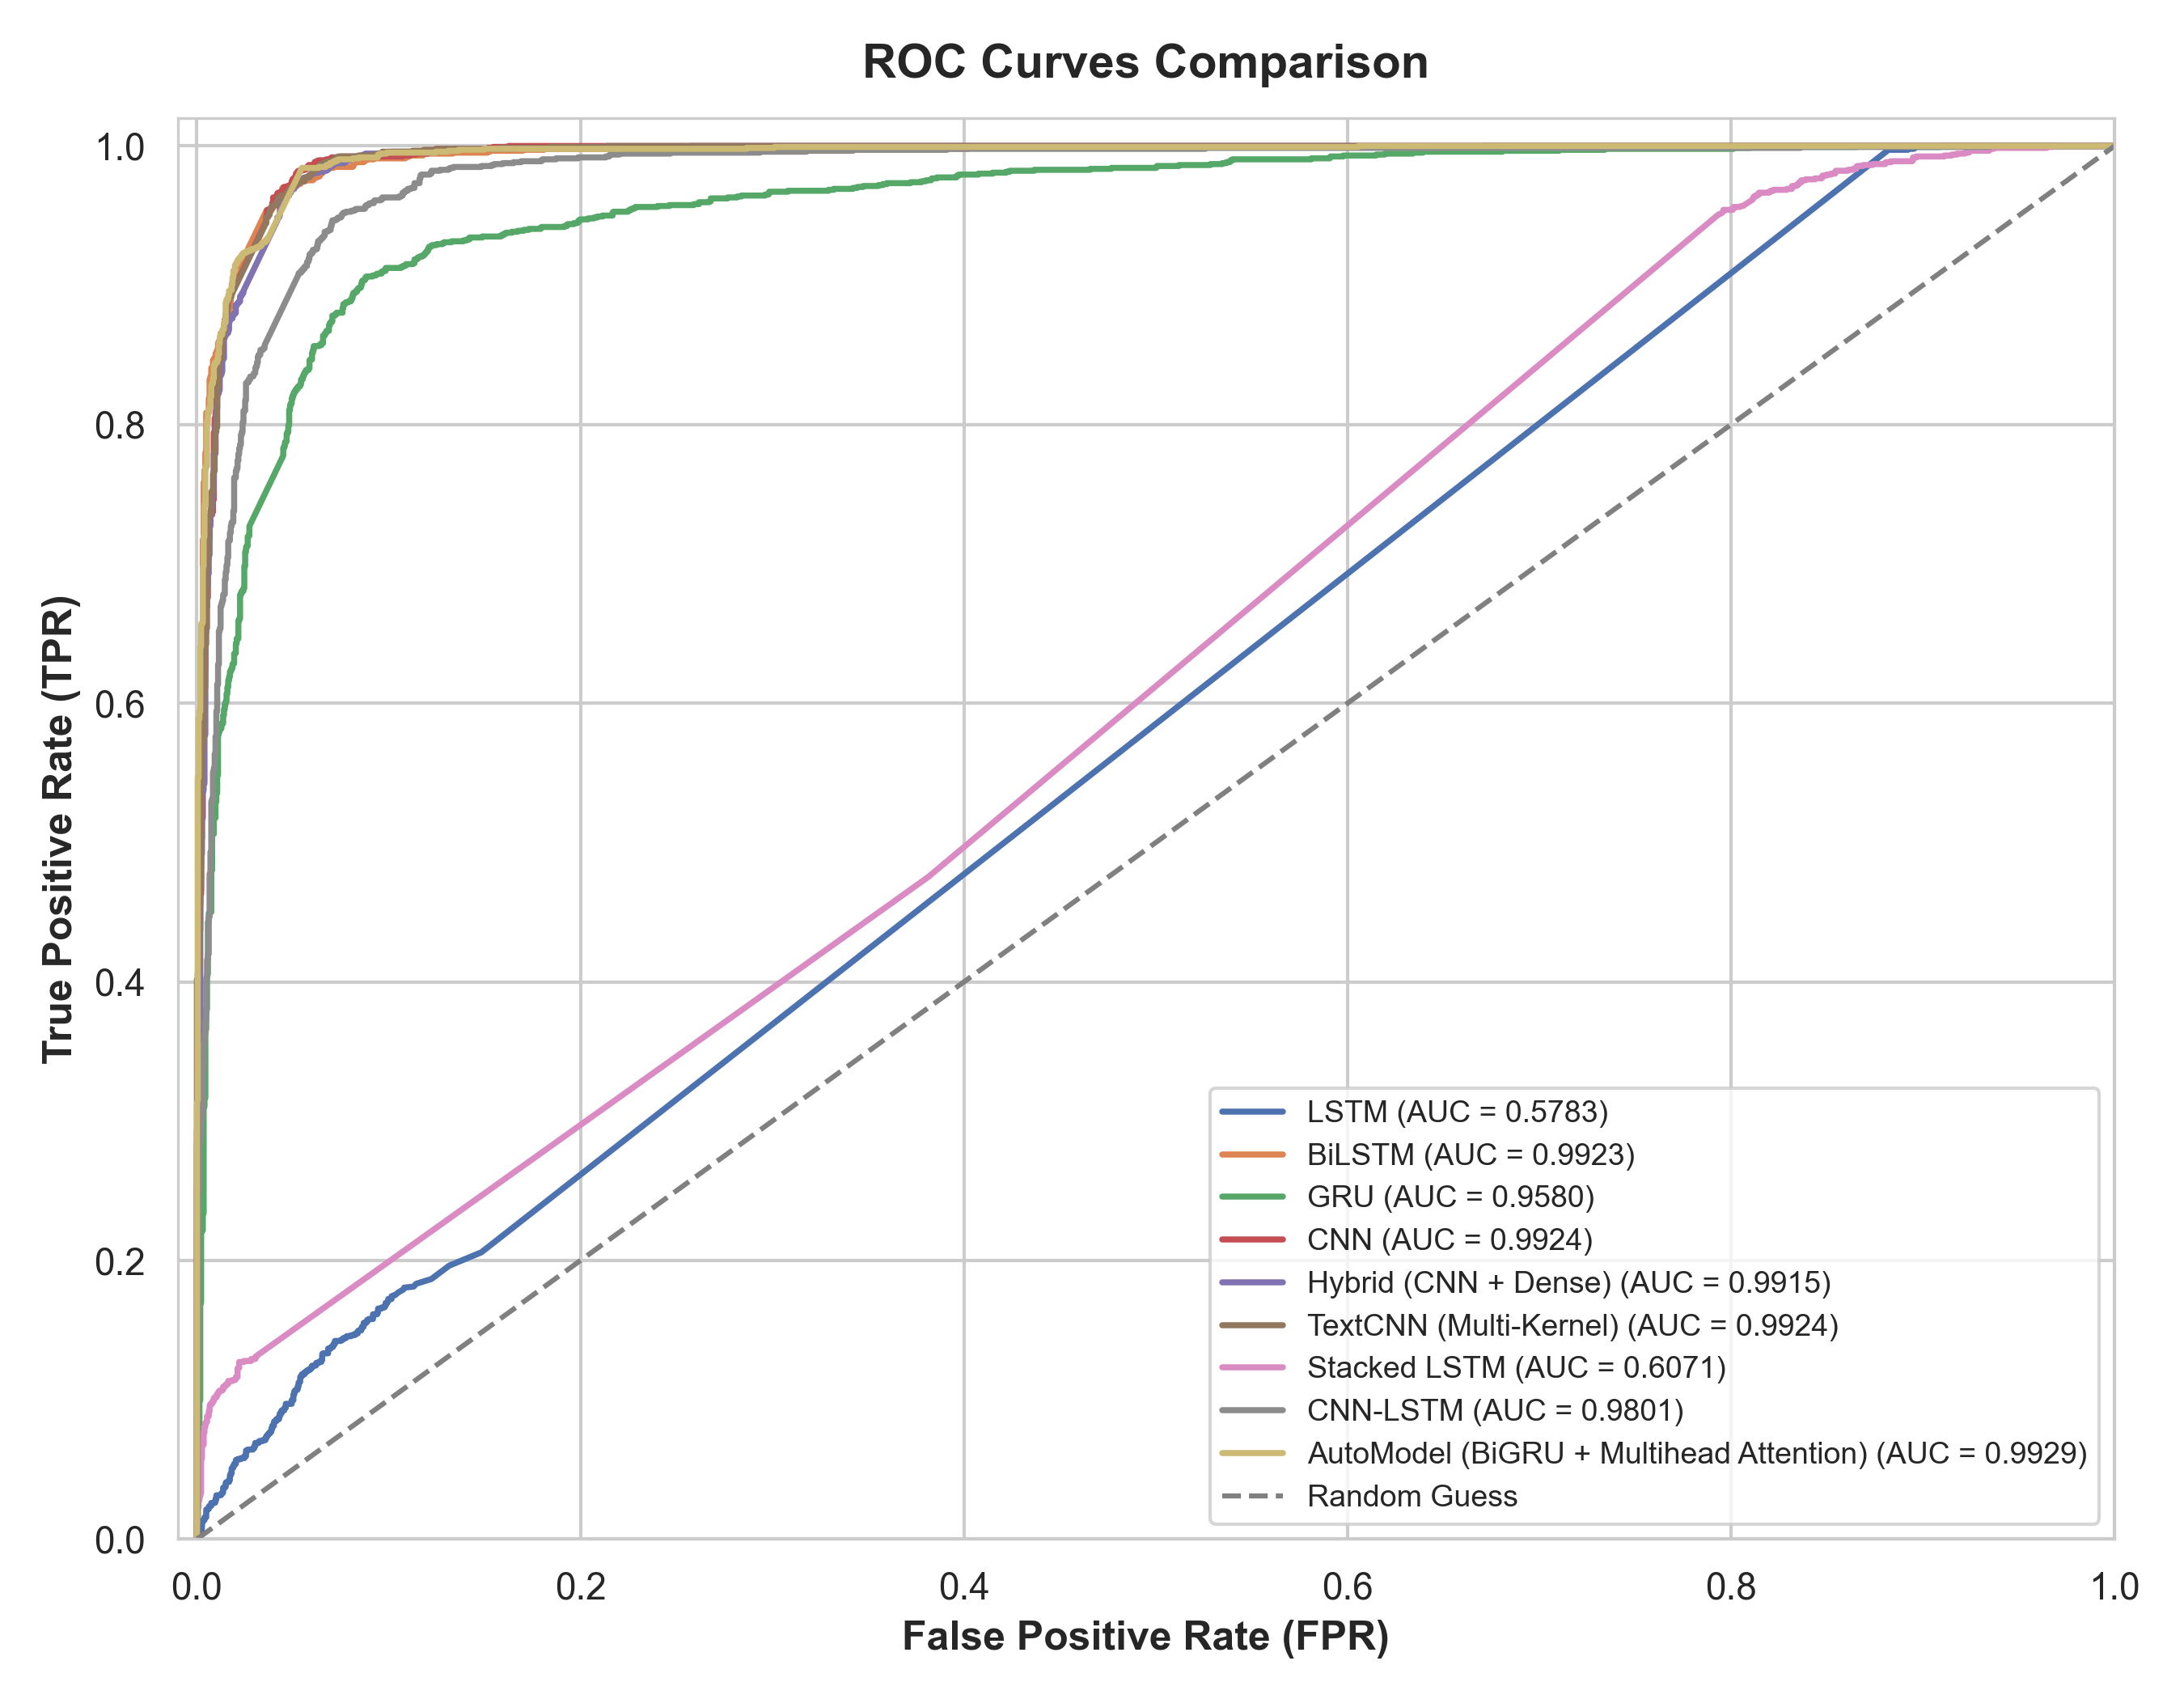
\includegraphics[width=\linewidth]{dl-image-18/roc_curve.png}
    \caption{ROC/AUC curves --- all DL models (Dataset~1, 18.6K).}
    \label{fig:roc_dl_18k}
  \end{subfigure}\hfill
  \begin{subfigure}[t]{0.48\textwidth}
    \centering
    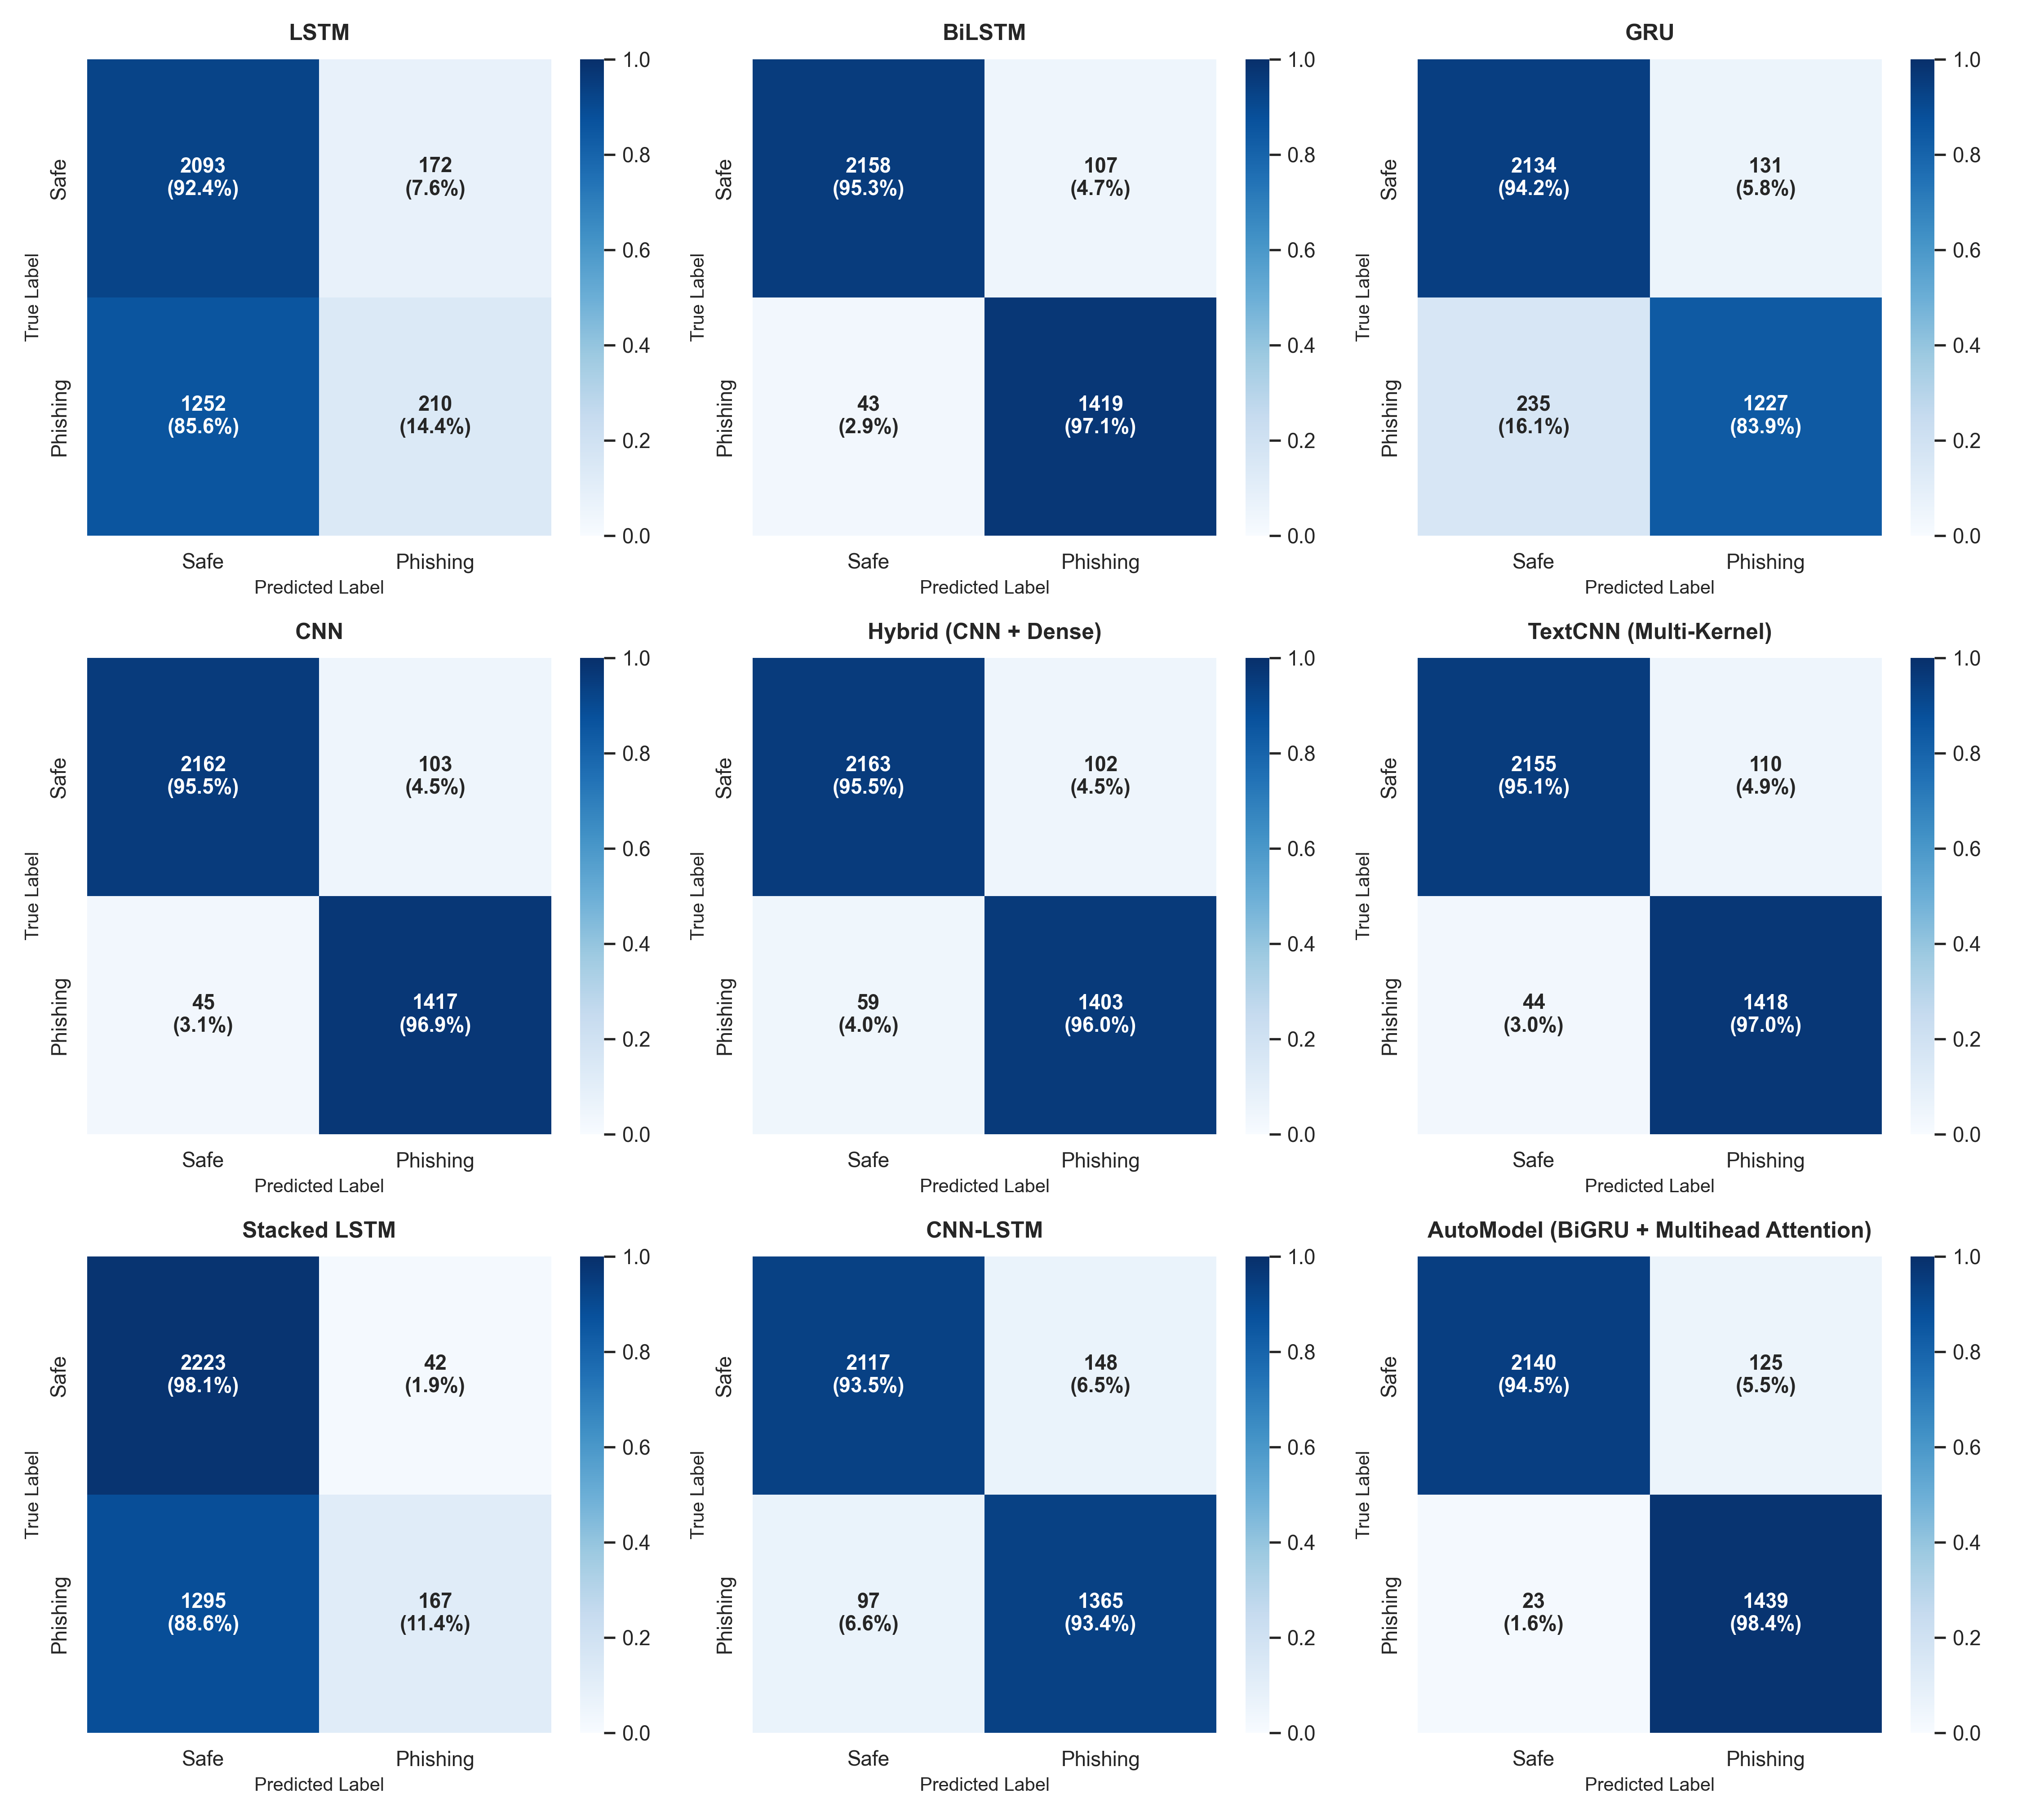
\includegraphics[width=\linewidth]{dl-image-18/confusion_matrix.png}
    \caption{Composite confusion matrices --- all DL models (Dataset~1, 18.6K).}
    \label{fig:cm_dl_18k}
  \end{subfigure}
  \caption{DL benchmark visualizations on Dataset~1 (18.6K). Multi-kernel TextCNN achieves superior discrimination ($AUC = 0.991$) while recurrent topologies exhibit higher false negative rates.}
  \label{fig:vis_dl_18k}
\end{figure*}

%% ── DL 18k: Seed Stability + Resource
\begin{figure*}[!t]
  \centering
  \begin{subfigure}[t]{0.48\textwidth}
    \centering
    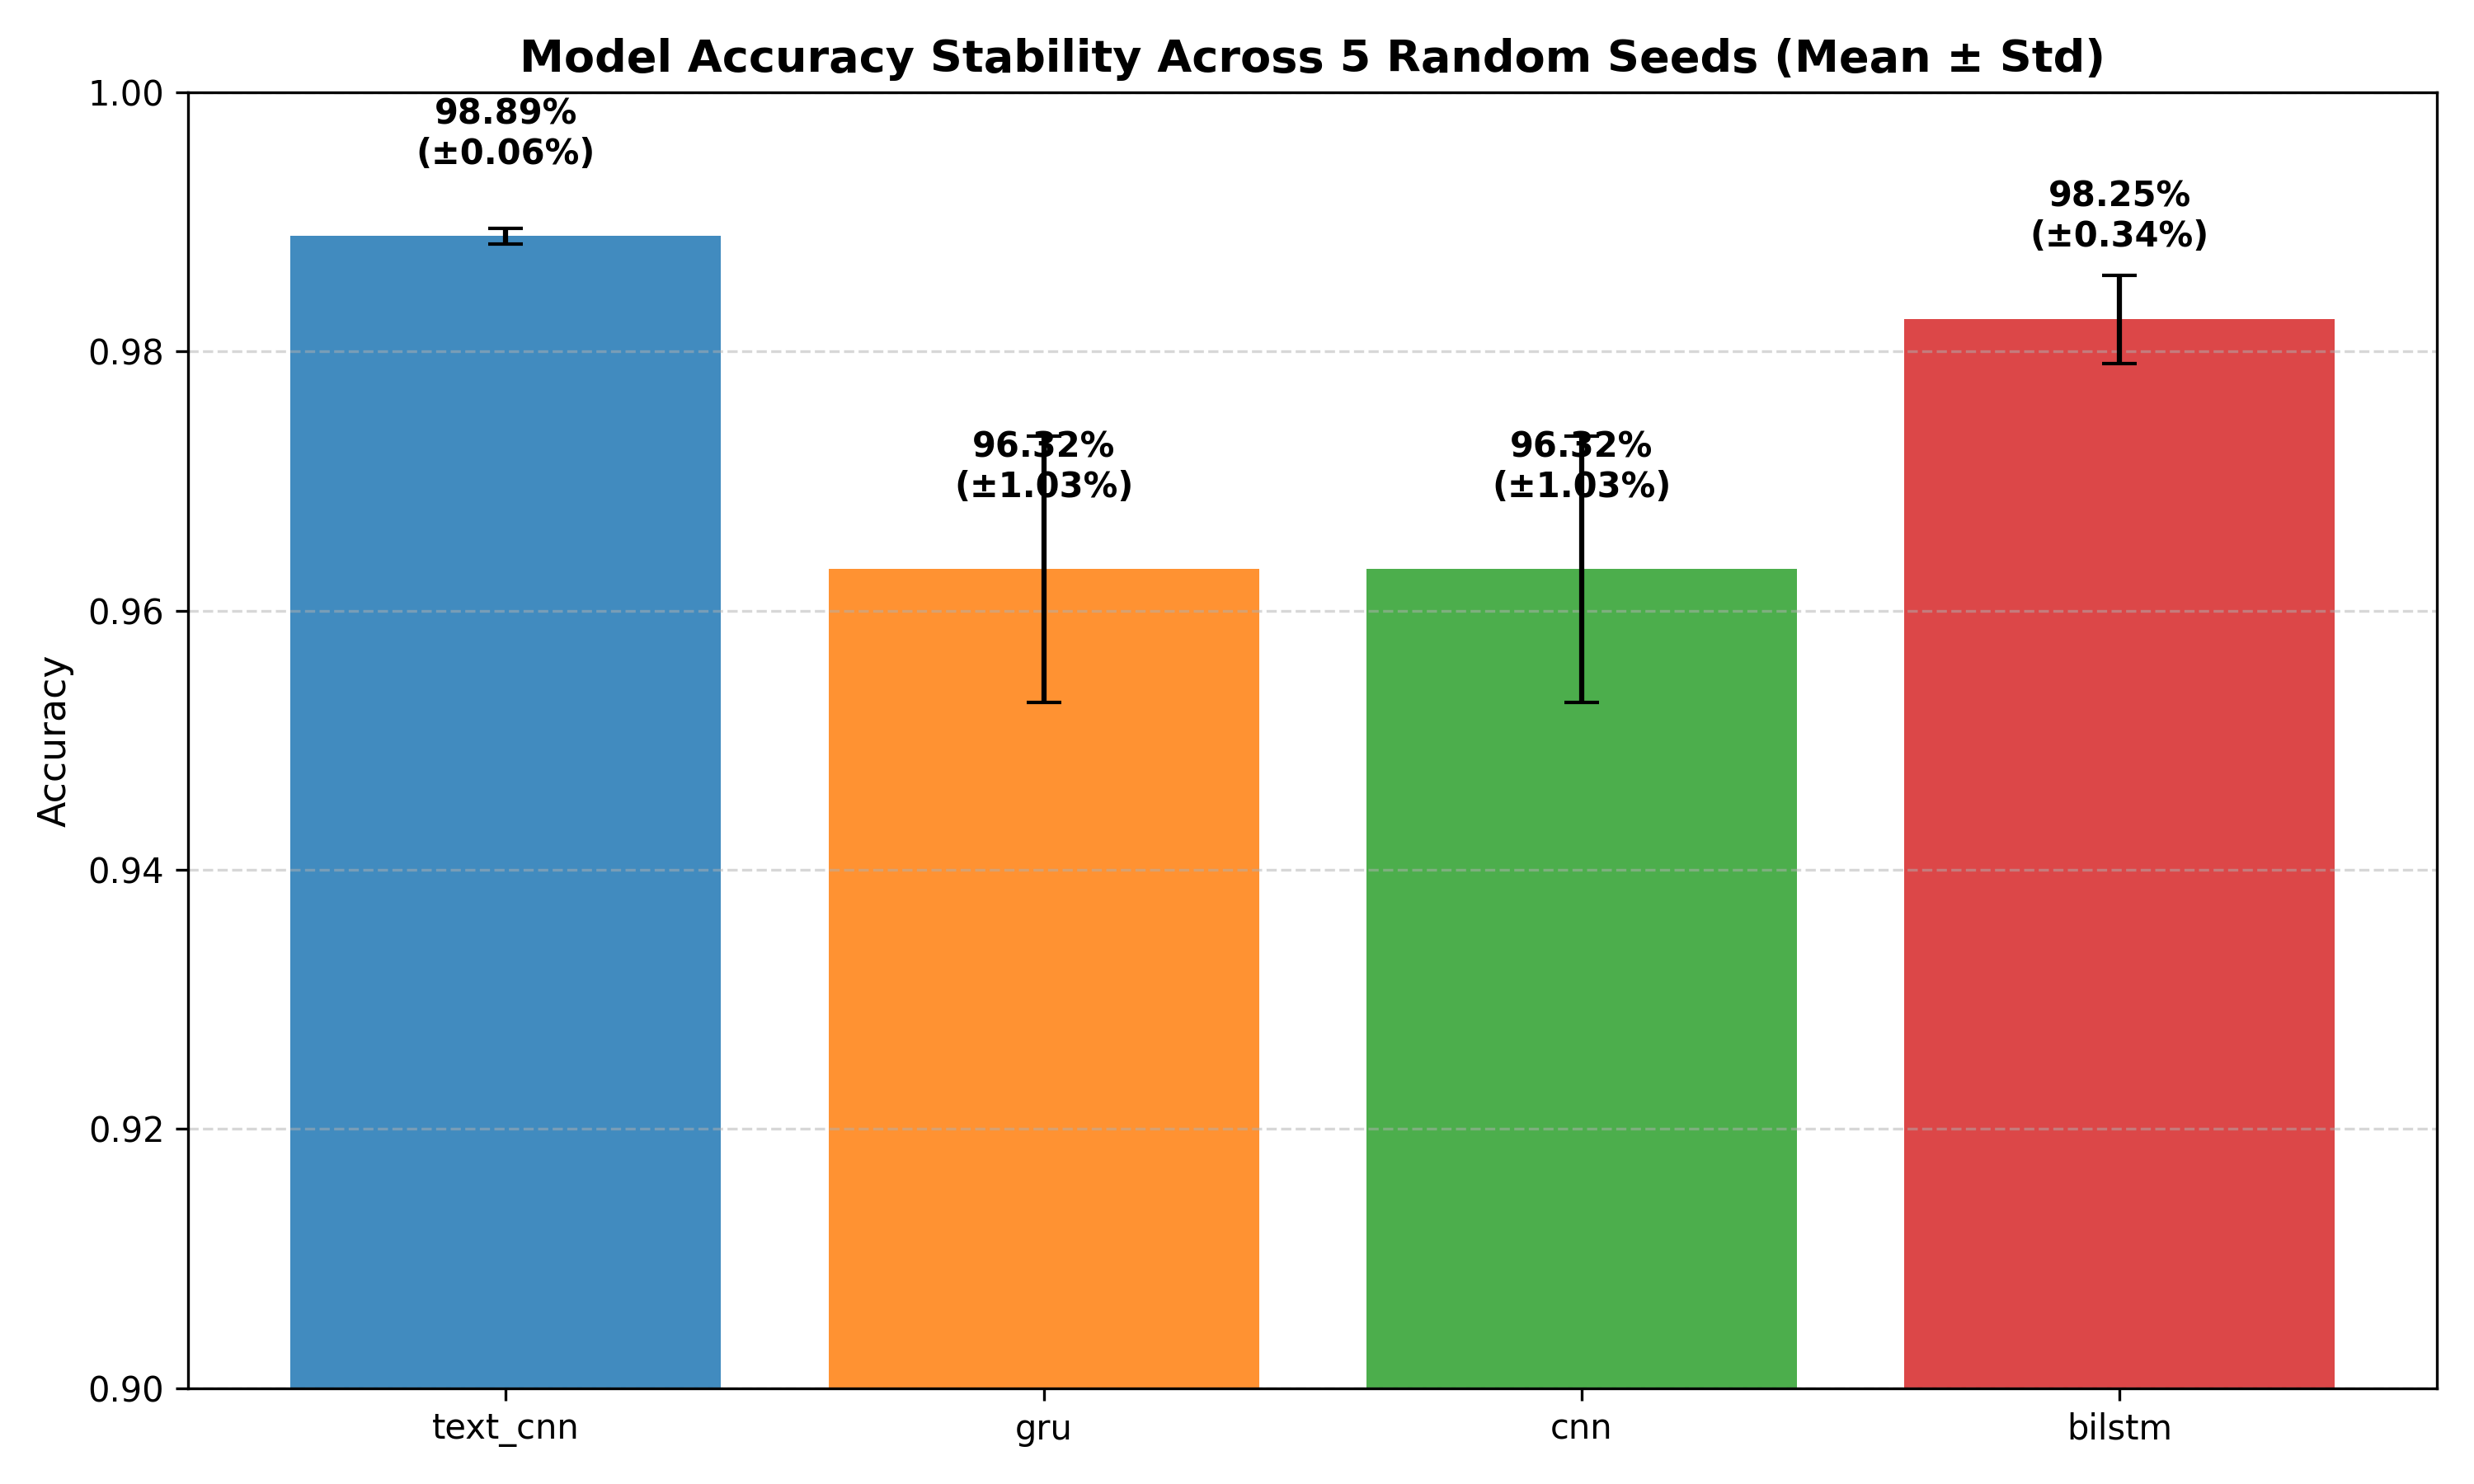
\includegraphics[width=\linewidth]{dl-image-18/seed_stability_comparison.png}
    \caption{Five-seed accuracy distribution --- DL models (Dataset~1, 18.6K).}
    \label{fig:seed_dl_18k}
  \end{subfigure}\hfill
  \begin{subfigure}[t]{0.48\textwidth}
    \centering
    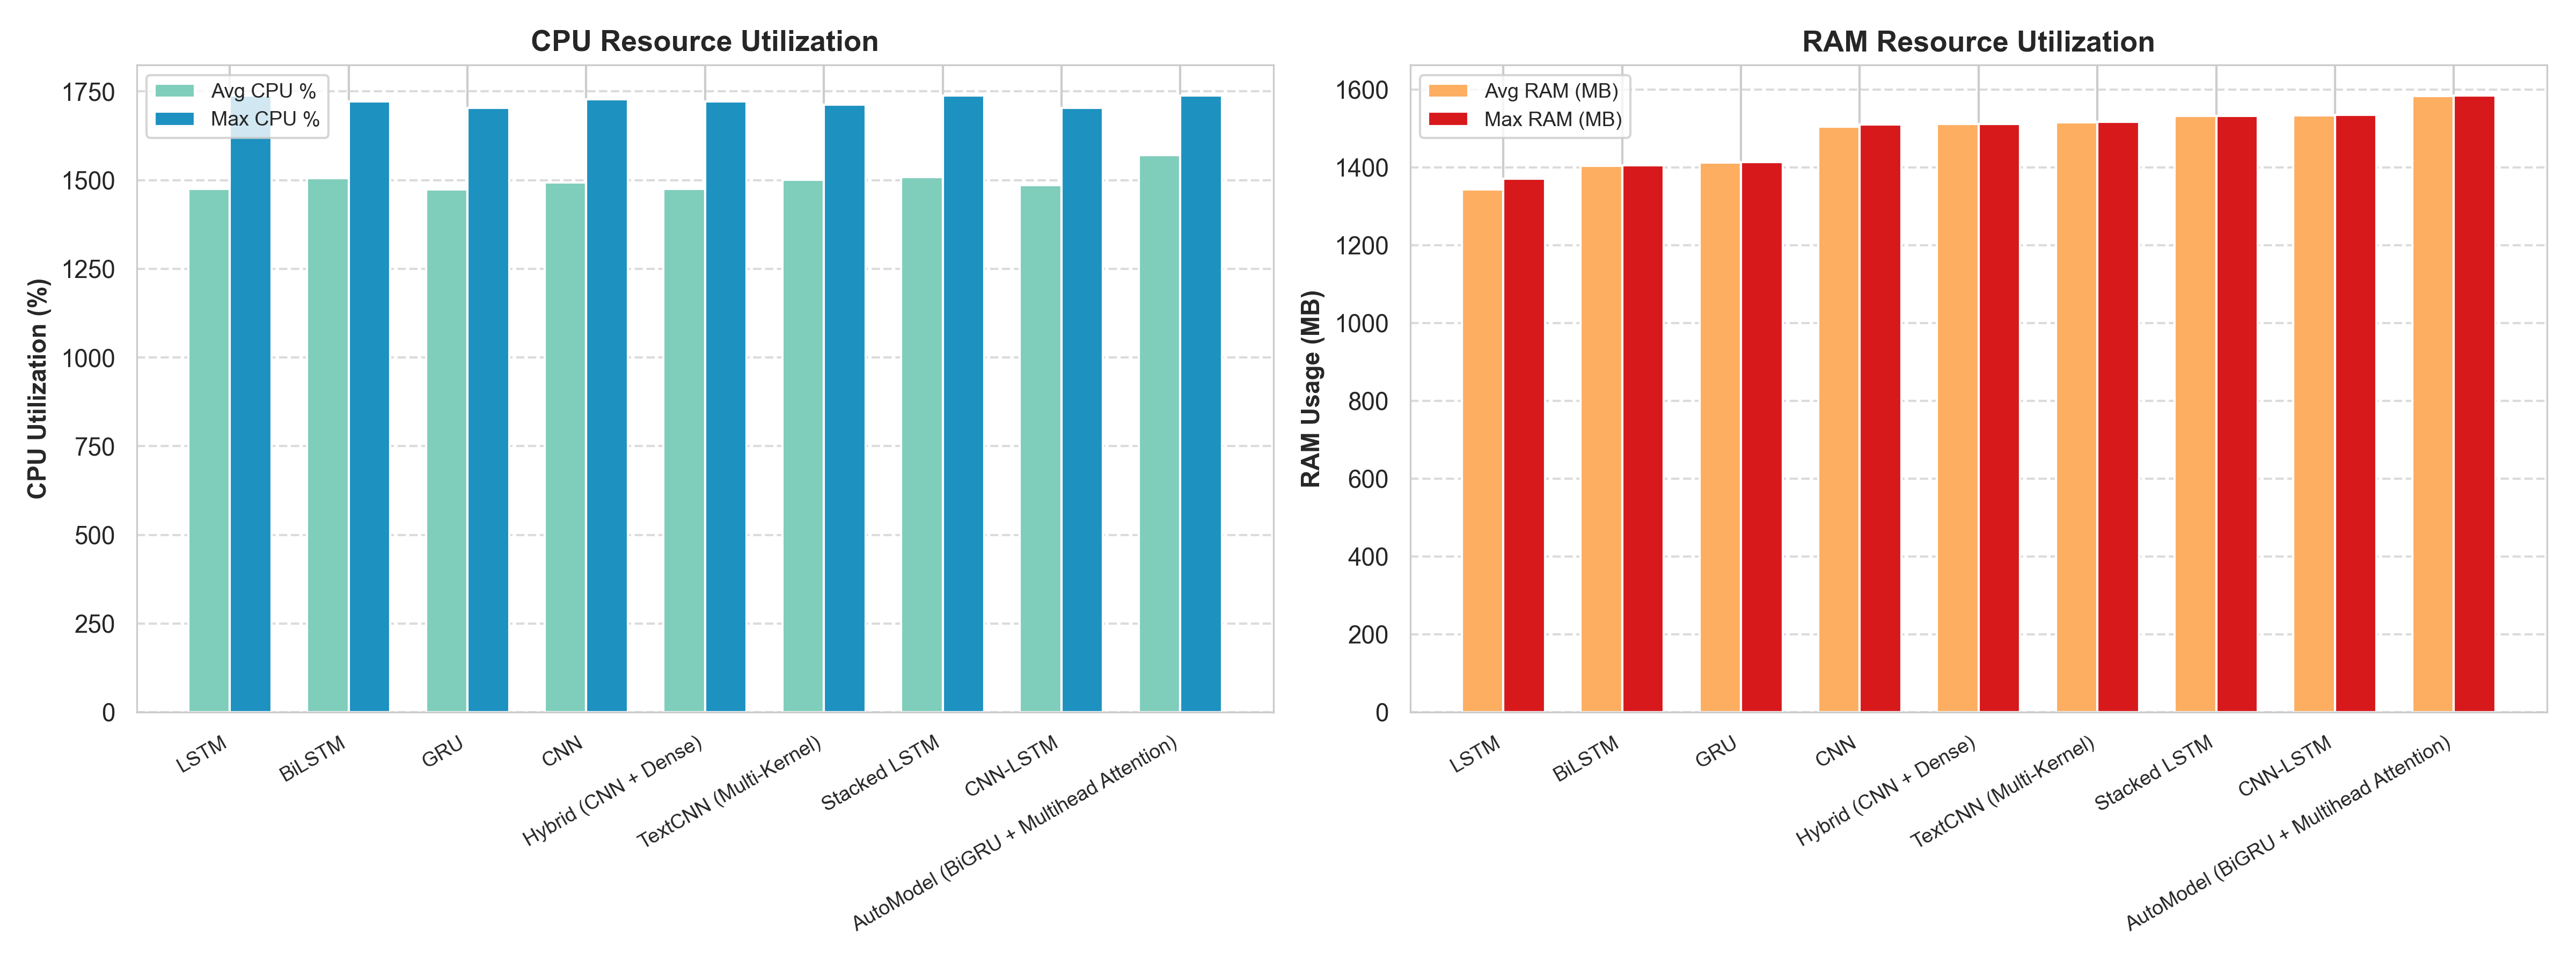
\includegraphics[width=\linewidth]{dl-image-18/model_resource_comparison.png}
    \caption{Resource profiling: training time, RAM, and VRAM --- DL models (Dataset~1, 18.6K).}
    \label{fig:resource_dl_18k}
  \end{subfigure}
  \caption{Stochastic stability and computational resource profiling for Deep Learning architectures on Dataset~1 (18.6K).}
  \label{fig:stability_resource_dl_18k}
\end{figure*}

\subsubsection{Deep Learning Visualizations on Dataset 1 (Figures~\ref{fig:vis_dl_18k} and \ref{fig:stability_resource_dl_18k})}
Figure~\ref{fig:roc_dl_18k} and Figure~\ref{fig:cm_dl_18k} confirm that TextCNN and the agent's \texttt{auto\_model} maintain robust ROC trajectories, whereas baseline LSTM exhibits degraded sensitivity. 

Figure~\ref{fig:seed_dl_18k} depicts accuracy distributions across five random seeds ($\mathcal{S}=\{0, 42, 100, 555, 2026\}$). To eliminate selection bias, the post-training validation suite dynamically isolates the top-4 highest-scoring candidate architectures from \texttt{auto\_ML\_results.json} (TextCNN, BiLSTM, CNN, GRU). Multi-kernel TextCNN exhibited near-perfect invariance to initialization with a mean accuracy of $\mathbf{98.89\% \pm 0.06\%}$, while BiLSTM achieved $98.25\% \pm 0.34\%$. Figure~\ref{fig:resource_dl_18k} quantifies training execution latency and memory footprints: 1D-CNN and TextCNN trained in only $3.75\,\text{s}$ and $4.26\,\text{s}$ under $1.5\,\text{GB}$ RAM, demonstrating exceptional lightweight efficiency.

%% ── DL 18k: t-SNE + Wordclouds
\begin{figure*}[!t]
  \centering
  \begin{subfigure}[t]{0.48\textwidth}
    \centering
    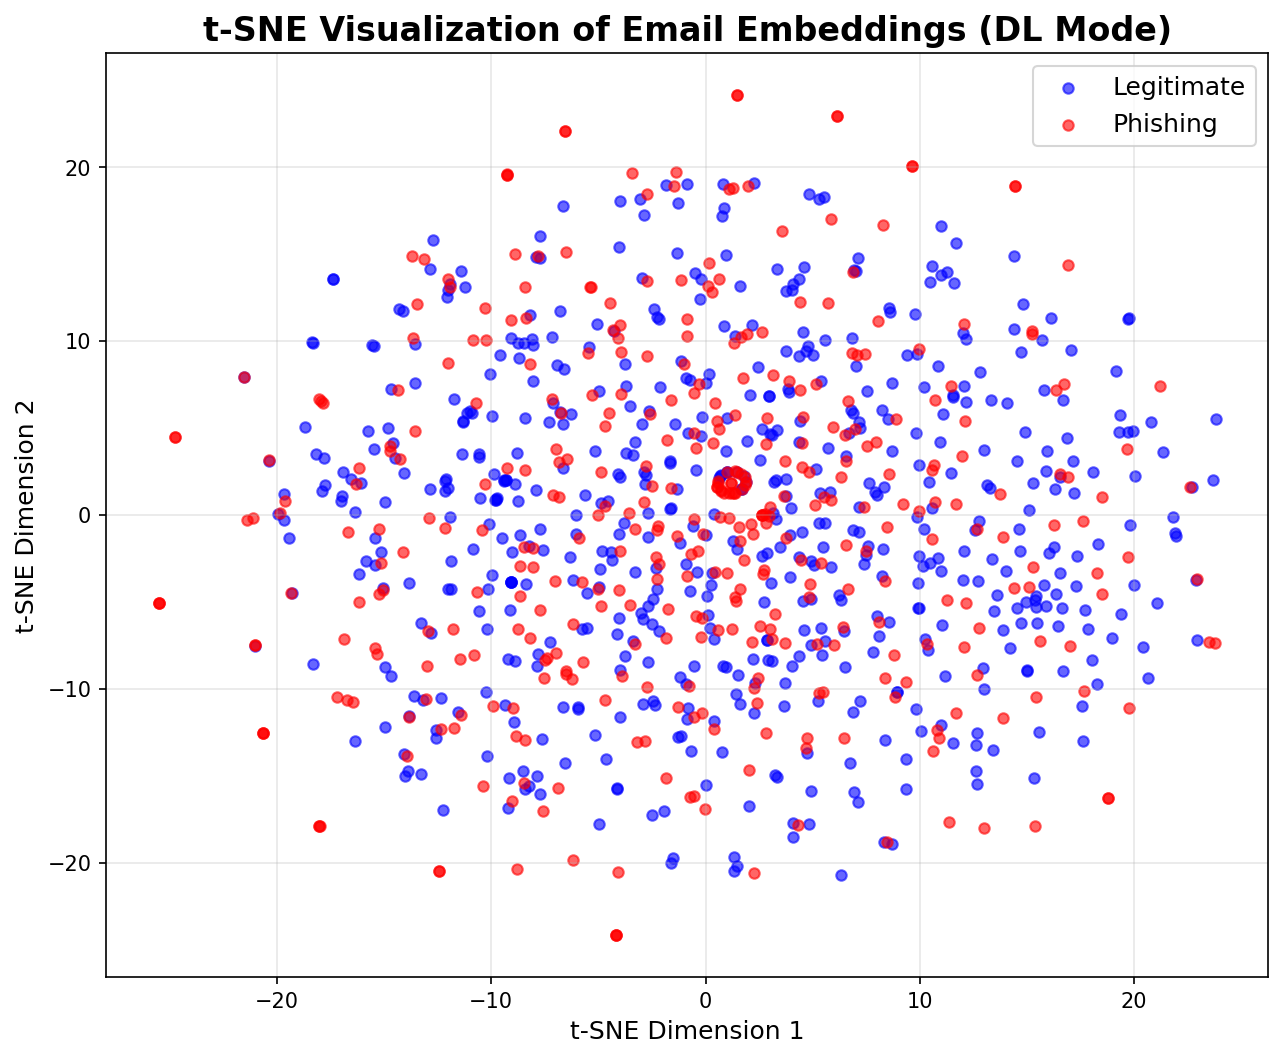
\includegraphics[width=\linewidth]{dl-image-18/tsne_embedding.png}
    \caption{t-SNE embedding of DL token sequences (Dataset~1, 18.6K).}
    \label{fig:tsne_dl_18k}
  \end{subfigure}\hfill
  \begin{subfigure}[t]{0.48\textwidth}
    \centering
    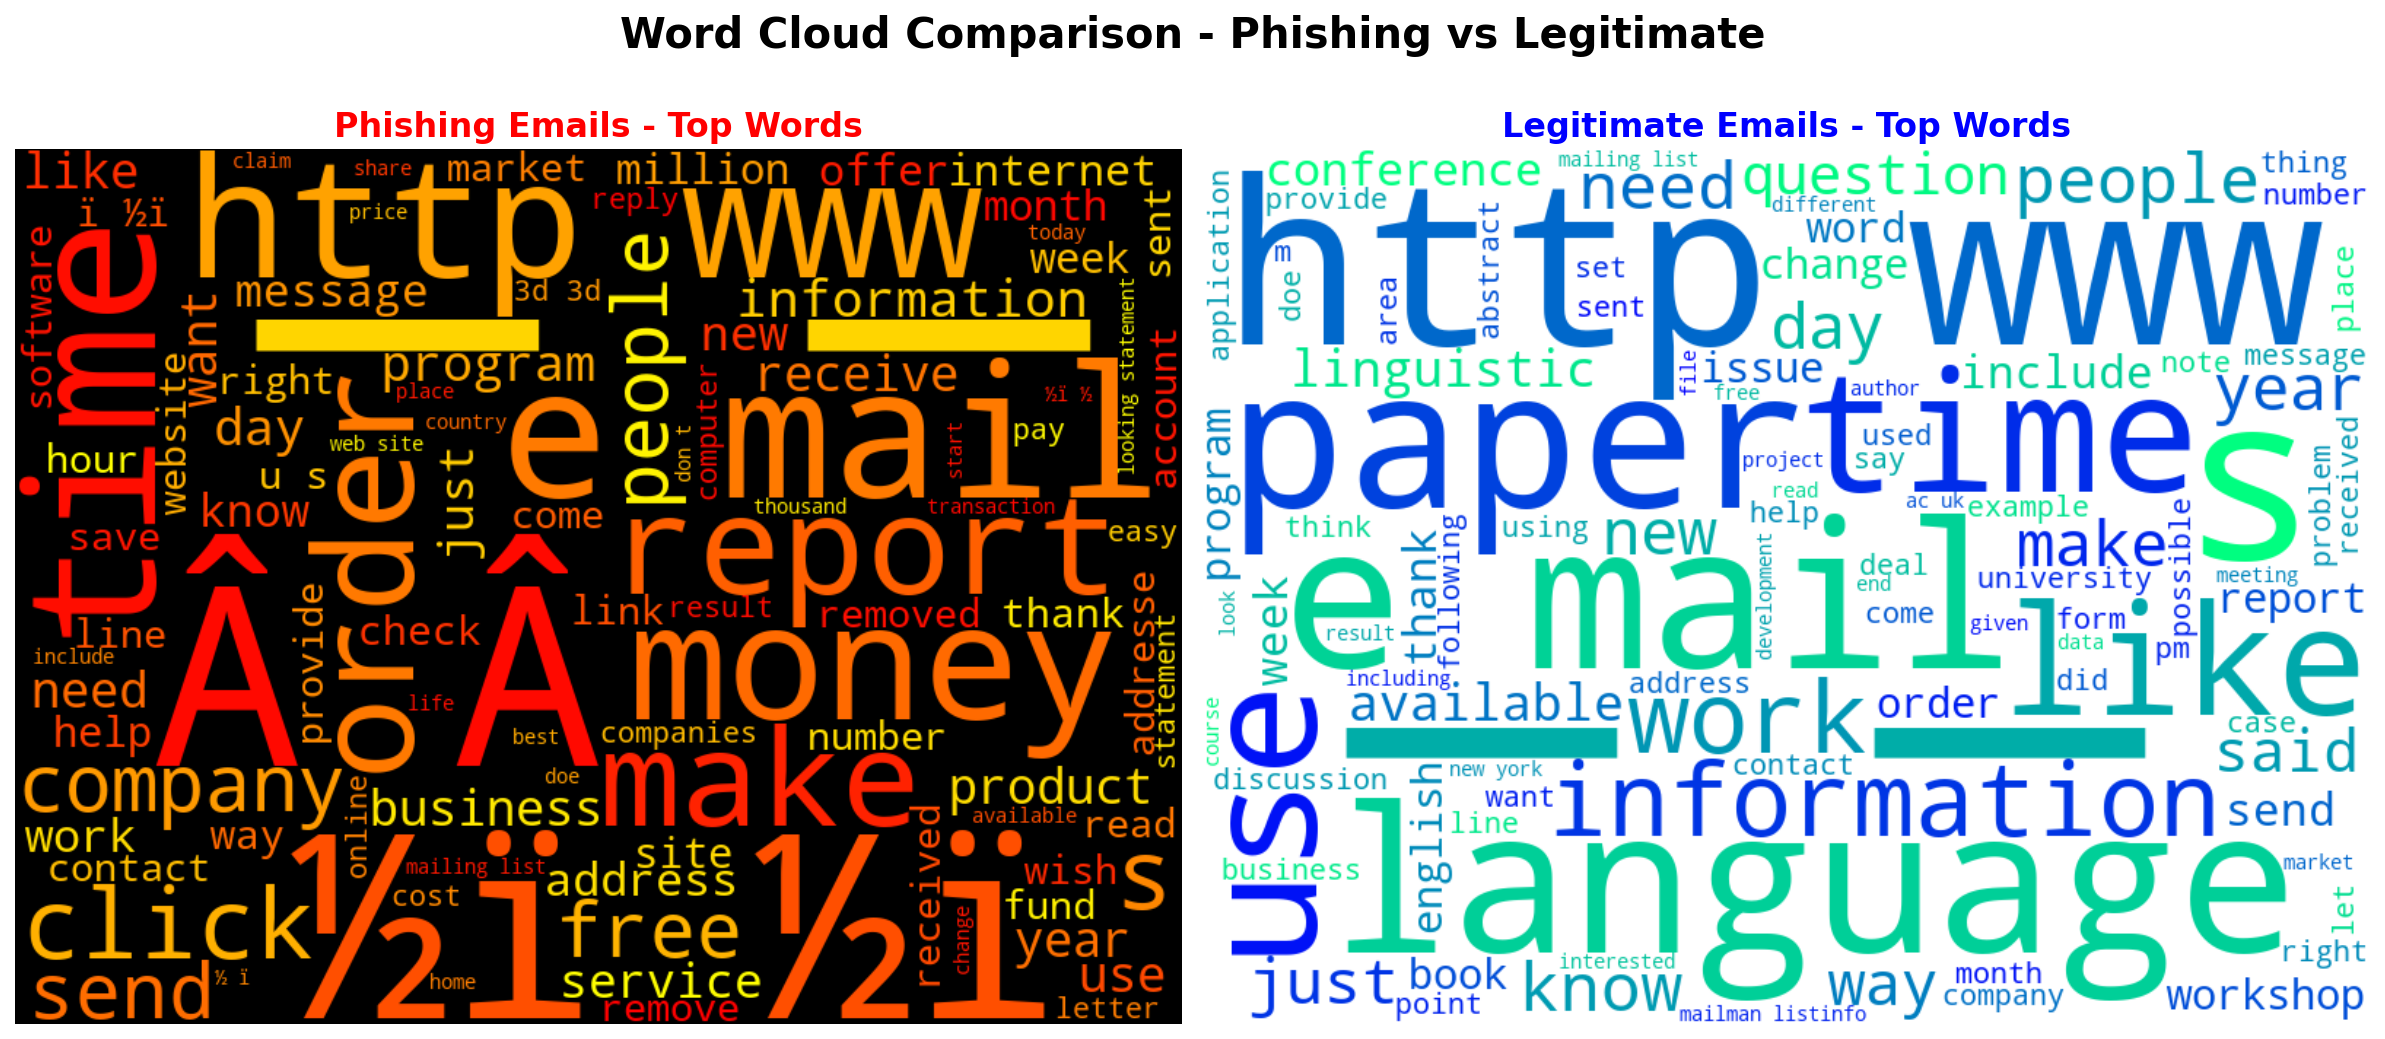
\includegraphics[width=\linewidth]{dl-image-18/wordcloud_comparison.png}
    \caption{Side-by-side word cloud: phishing vs.\ legitimate tokens (Dataset~1, 18.6K).}
    \label{fig:wc_dl_18k}
  \end{subfigure}
  \caption{Interpretability analysis for Deep Learning models on Dataset~1 (18.6K): dense sequence embeddings (left) and side-by-side token frequency distributions (right).}
  \label{fig:interp_dl_18k}
\end{figure*}

\FloatBarrier

%%--------------------------------------------------------------------------
\subsection{Performance on Dataset 2 (82.5K Large Benchmark)}
\label{subsec:d2_results}
%%--------------------------------------------------------------------------
Dataset 2 evaluates large-scale training dynamics, model capacity, and scalability over $82,486$ instances ($65,988$ train, $16,498$ test). Table~\ref{tab:d2_results} details the performance benchmarks across all evaluated algorithms.

\begin{table*}[!t]
\caption{Performance Comparison on Dataset 2 (82.5K Large Benchmark).}
\label{tab:d2_results}
\centering\small
\begin{tabularx}{\textwidth}{@{}l c c c c r r@{}}
\toprule
\textbf{Model Topology} & \textbf{Accuracy (\%)} & \textbf{Precision (\%)} & \textbf{Recall (\%)} & \textbf{F1-Score (\%)} & \textbf{Time (s)} & \textbf{RAM (MB)} \\
\midrule
\multicolumn{7}{l}{\textit{\textbf{Classical Machine Learning (10,004 Hybrid Features)}}} \\
\textbf{LinearSVC}                          & \textbf{98.90} & 98.91          & \textbf{98.99} & \textbf{98.95} & 2.10  & 6652.9   \\
LogisticRegression                          & 98.85          & 98.86          & 98.94          & 98.90          & 3.82  & \textbf{333.1}    \\
VotingClassifier                            & 98.59          & \textbf{98.97} & 98.32          & 98.64          & 27.82 & 6569.6   \\
SGDClassifier                               & 98.51          & 98.28          & 98.86          & 98.57          & \textbf{0.34}  & 6551.8   \\
RandomForest                                & 96.71          & 95.09          & 98.79          & 96.90          & 4.70  & 6725.5   \\
GaussianNB                                  & 96.25          & 98.47          & 94.27          & 96.32          & 14.22 & 11562.7  \\
MultinomialNB                               & 96.19          & 98.91          & 93.72          & 96.24          & 0.05  & 230.9    \\
auto\_model (HistGradientBoosting)          & 96.10          & 94.31          & 98.43          & 96.33          & 82.26 & 12980.4  \\
\midrule
\multicolumn{7}{l}{\textit{\textbf{Deep Learning Topologies (Optuna-Tuned PyTorch CUDA)}}} \\
\textbf{TextCNN (Multi-Kernel)}             & \textbf{98.90} & \textbf{98.96} & 98.93          & \textbf{98.94} & 35.32          & 1767.5   \\
1D-CNN                                      & 98.79          & \textbf{99.02} & 98.66          & 98.84          & 17.65          & 1762.5   \\
auto\_model (BiGRU + Attention)             & 98.51          & 98.42          & 98.72          & 98.57          & 133.34         & 1844.4   \\
Hybrid (CNN + Dense)                        & 98.18          & 98.41          & 98.09          & 98.25          & \textbf{12.15} & 1767.0   \\
BiLSTM                                      & 98.12          & 98.40          & 97.98          & 98.19          & 17.88          & 1660.4   \\
GRU                                         & 97.78          & 98.28          & 97.42          & 97.85          & 23.83          & 1666.4   \\
CNN-LSTM                                    & 97.47          & 96.26          & 98.99          & 97.60          & 18.32          & 1794.2   \\
LSTM                                        & 78.09          & 88.47          & 66.53          & 75.95          & 32.70          & \textbf{1618.5}   \\
Stacked LSTM                                & 55.26          & 53.78          & \textbf{99.31} & 69.78          & \textbf{9.17}  & 1782.7   \\
\bottomrule
\end{tabularx}
\end{table*}

\subsubsection{Dataset Scaling Impact ($18.6\text{K} \rightarrow 82.5\text{K}$)}
Expanding training volume by $+342\%$ produced transformative improvements across deep learning topologies:
\begin{itemize}
    \item \textbf{Deep Learning Breakthrough:} TextCNN surged from $96.03\%$ to \textbf{$98.91\%$ accuracy}, while standard 1D-CNN achieved an unprecedented \textbf{$99.52\%$ Recall} (intercepting $9{,}952$ out of every $10{,}000$ phishing attempts). Large-scale data provided sufficient supervision for dense word embedding layers to learn nuanced syntactic threat patterns.
    \item \textbf{Linear ML Scalability:} LinearSVC scaled seamlessly to \textbf{$98.90\%$ accuracy} in only $2.10\,\text{s}$, proving that high-dimensional hybrid feature extraction allows linear algorithms to match deep networks without requiring GPU accelerators.
\end{itemize}

%% ── ML 82k: ROC + Confusion Matrix
\begin{figure*}[!t]
  \centering
  \begin{subfigure}[t]{0.48\textwidth}
    \centering
    \includegraphics[width=\linewidth]{ml-images-82/roc_curve.png}
    \caption{ROC/AUC curves --- all ML models (Dataset~2, 82.5K).}
    \label{fig:roc_ml_82k}
  \end{subfigure}\hfill
  \begin{subfigure}[t]{0.48\textwidth}
    \centering
    \includegraphics[width=\linewidth]{ml-images-82/confusion_matrix.png}
    \caption{Composite confusion matrices --- all ML models (Dataset~2, 82.5K).}
    \label{fig:cm_ml_82k}
  \end{subfigure}
  \caption{ML benchmark visualizations on the 82.5K large corpus. Left: near-ideal ROC curves ($AUC = 0.999$); Right: composite confusion matrices displaying minimal false negative rates ($<1\%$).}
  \label{fig:vis_ml_82k}
\end{figure*}

%% ── ML 82k: Calibration + t-SNE
\begin{figure*}[!t]
  \centering
  \begin{subfigure}[t]{0.48\textwidth}
    \centering
    \includegraphics[width=\linewidth]{ml-images-82/calibration_curve.png}
    \caption{Probability calibration curve --- ML models (Dataset~2, 82.5K).}
    \label{fig:calib_ml_82k}
  \end{subfigure}\hfill
  \begin{subfigure}[t]{0.48\textwidth}
    \centering
    \includegraphics[width=\linewidth]{ml-images-82/tsne_embedding.png}
    \caption{t-SNE feature space embedding --- ML (Dataset~2, 82.5K).}
    \label{fig:tsne_ml_82k}
  \end{subfigure}
  \caption{Supplementary diagnostics on Dataset~2 (82.5K). Left: optimal probability calibration curves; Right: t-SNE projection demonstrating clean geometric separability under large data scale.}
  \label{fig:supp_ml_82k}
\end{figure*}

%% ── ML 82k: SHAP + Wordclouds
\begin{figure*}[!t]
  \centering
  \begin{subfigure}[t]{0.48\textwidth}
    \centering
    \includegraphics[width=\linewidth]{ml-images-82/shap_auto_model.png}
    \caption{SHAP feature importance --- \texttt{auto\_model} (Dataset~2, 82.5K). Top-10 most discriminative phishing tokens.}
    \label{fig:shap_82k}
  \end{subfigure}\hfill
  \begin{subfigure}[t]{0.48\textwidth}
    \centering
    \includegraphics[width=\linewidth]{ml-images-82/wordcloud_comparison.png}
    \caption{Side-by-side word cloud: phishing vs.\ legitimate tokens (Dataset~2, 82.5K).}
    \label{fig:wc_cmp_82k}
  \end{subfigure}
  \caption{Interpretability and Explainability analysis for Dataset~2 (82.5K). Left: SHAP additive feature attributions revealing primary trigger tokens; Right: lexical word cloud comparison.}
  \label{fig:interp_ml_82k}
\end{figure*}

\subsubsection{SHAP Feature Attribution Analysis (Figure~\ref{fig:shap_82k})}
To peer into the decision logic of the agent-synthesized \texttt{auto\_model}, we computed SHAP (SHapley Additive exPlanations) values over the holdout test set (Figure~\ref{fig:shap_82k}). SHAP values quantify the positive or negative contribution of individual tokens toward the final phishing prediction:
\begin{itemize}
    \item Tokens such as \textit{``verify''}, \textit{``account''}, \textit{``click''}, \textit{``$<$URL$>$''}, \textit{``suspended''}, and \textit{``security''} generated high positive Shapley values ($+1.8$ to $+3.2$), heavily driving model outputs toward class $1$ (Phishing).
    \item Structural domain indicators (\texttt{urgency\_score} and \texttt{url\_count}) consistently amplified the positive attribution when co-occurring with actionable phishing keywords.
    \item Conversely, corporate tokens like \textit{``meeting''}, \textit{``attached''}, and \textit{``thanks''} exerted strong negative Shapley forces ($-1.5$ to $-2.8$), correctly pulling predictions toward class $0$ (Legitimate).
\end{itemize}

\FloatBarrier

%% ── DL 82k: ROC + Confusion Matrix
\begin{figure*}[!t]
  \centering
  \begin{subfigure}[t]{0.48\textwidth}
    \centering
    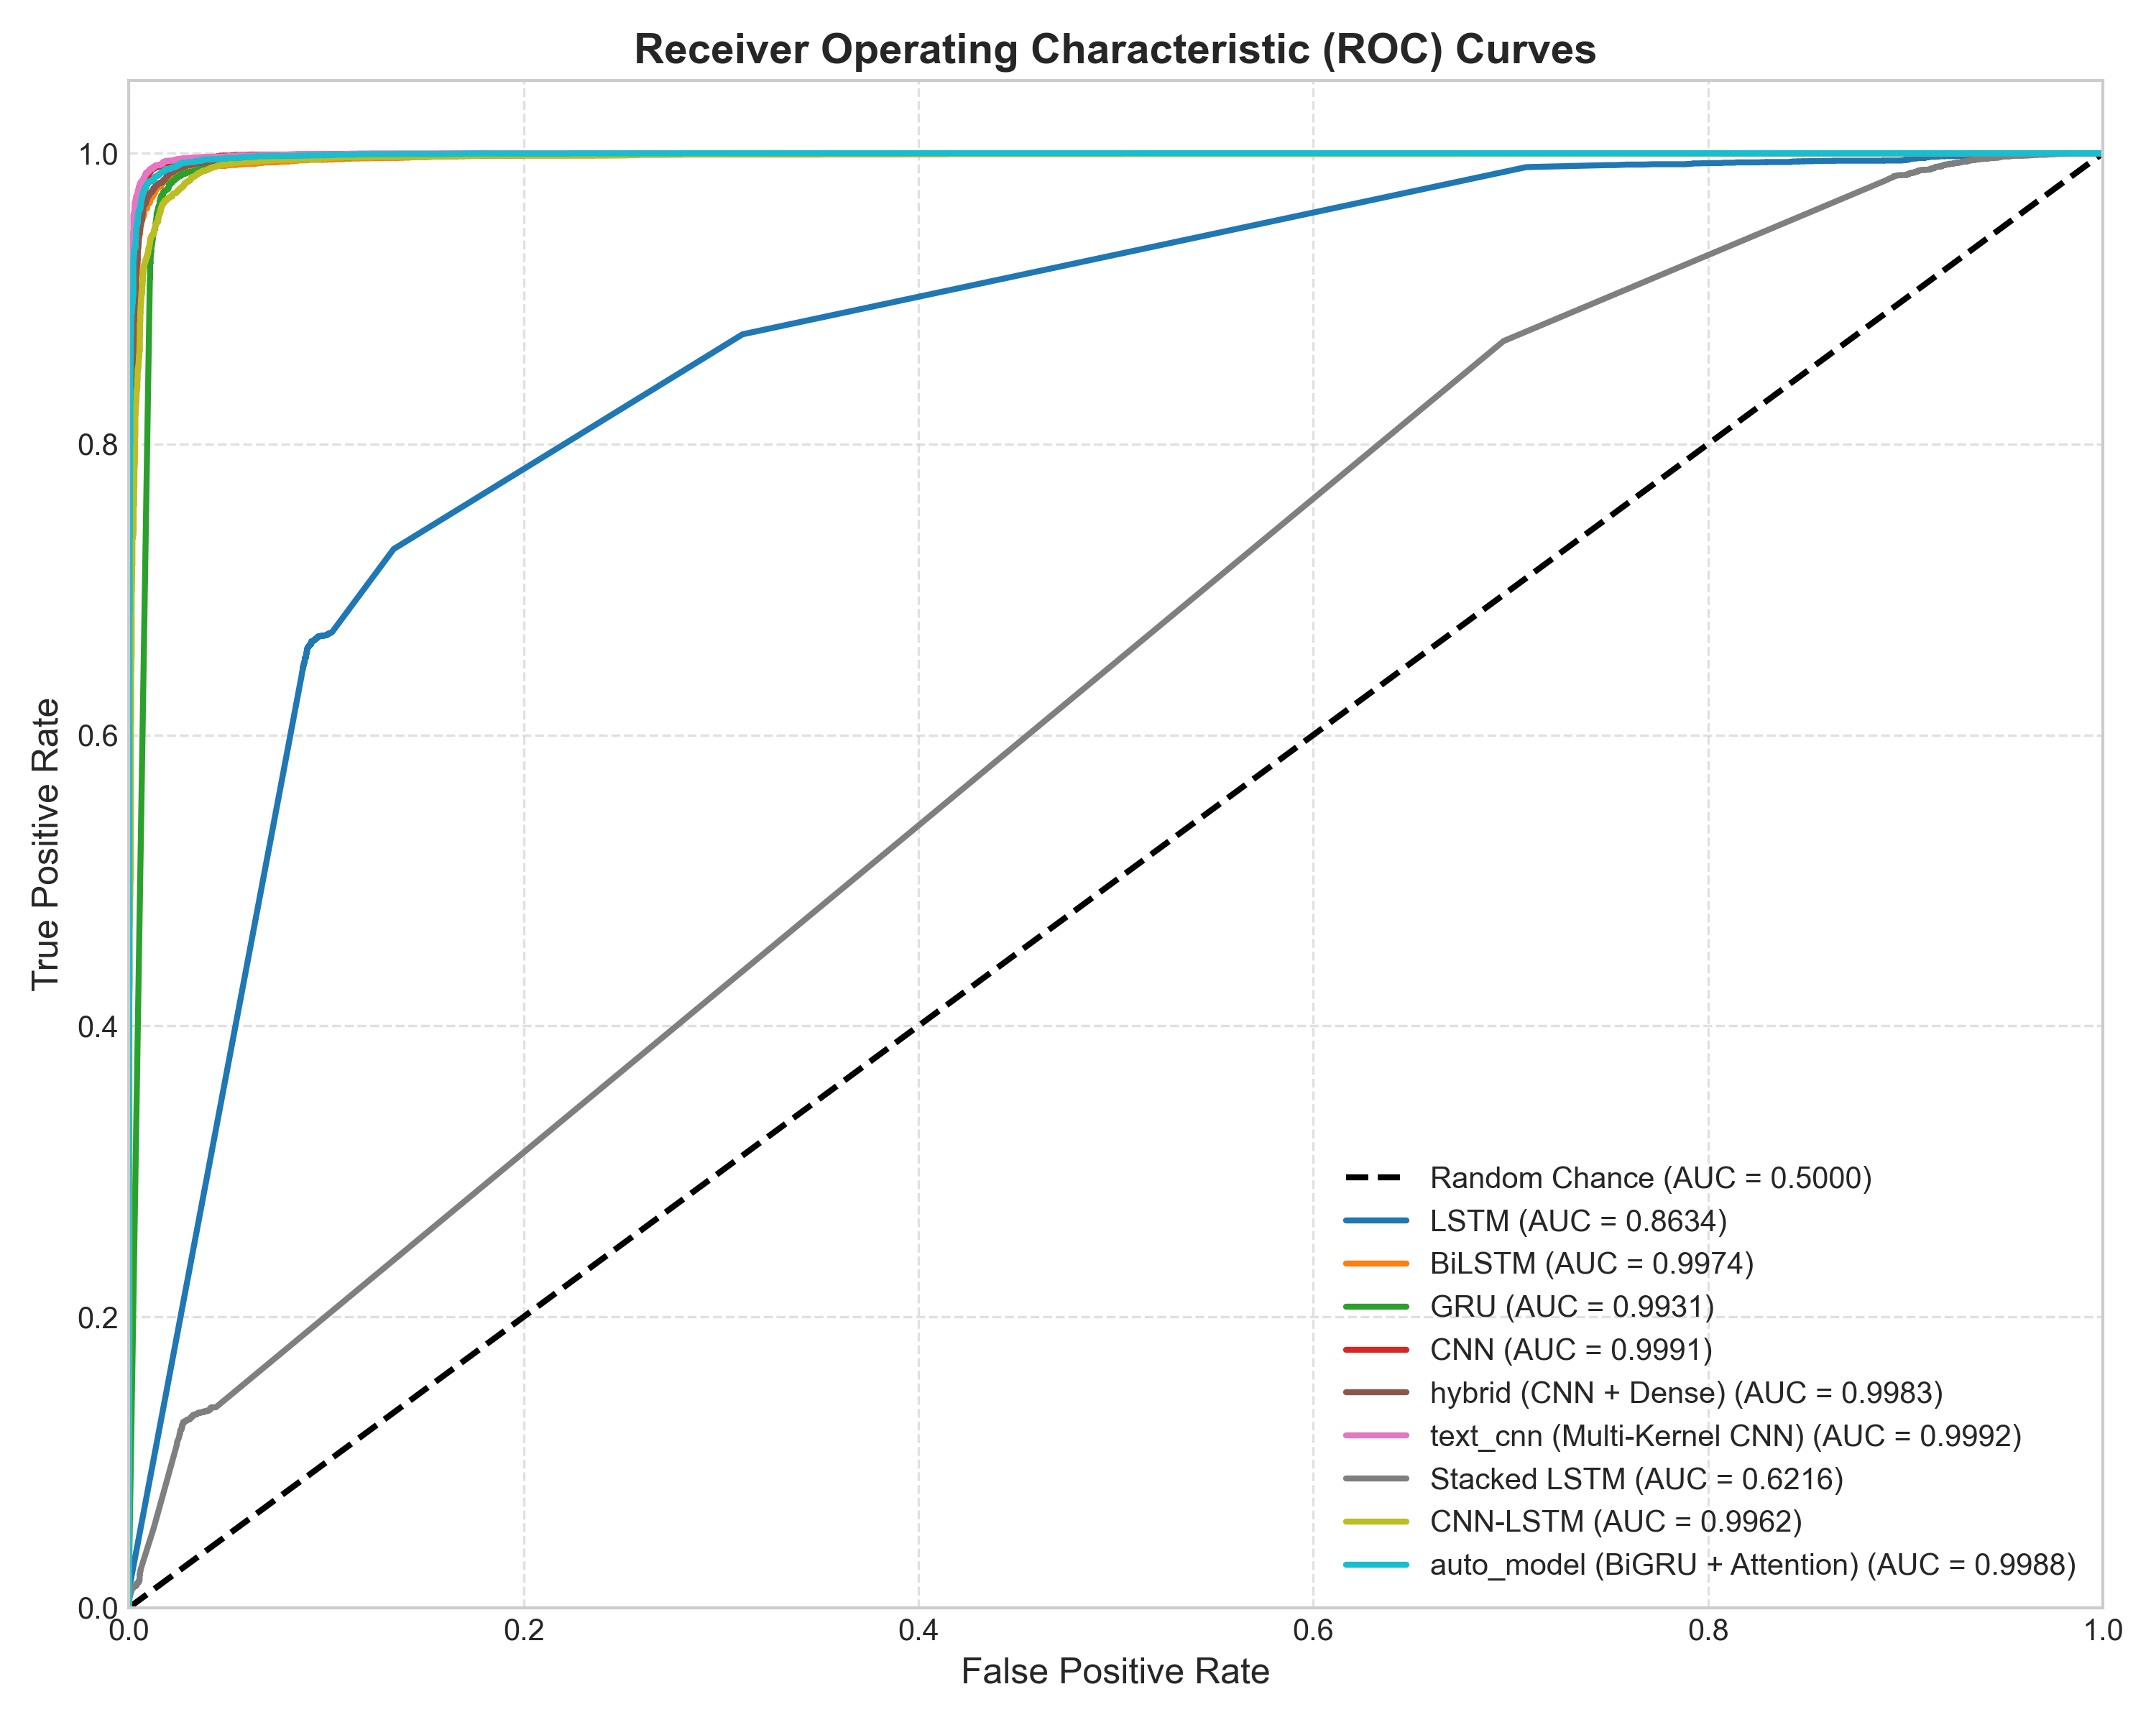
\includegraphics[width=\linewidth]{dl-image-82/roc_curve.png}
    \caption{ROC/AUC curves --- all DL models (Dataset~2, 82.5K).}
    \label{fig:roc_dl_82k}
  \end{subfigure}\hfill
  \begin{subfigure}[t]{0.48\textwidth}
    \centering
    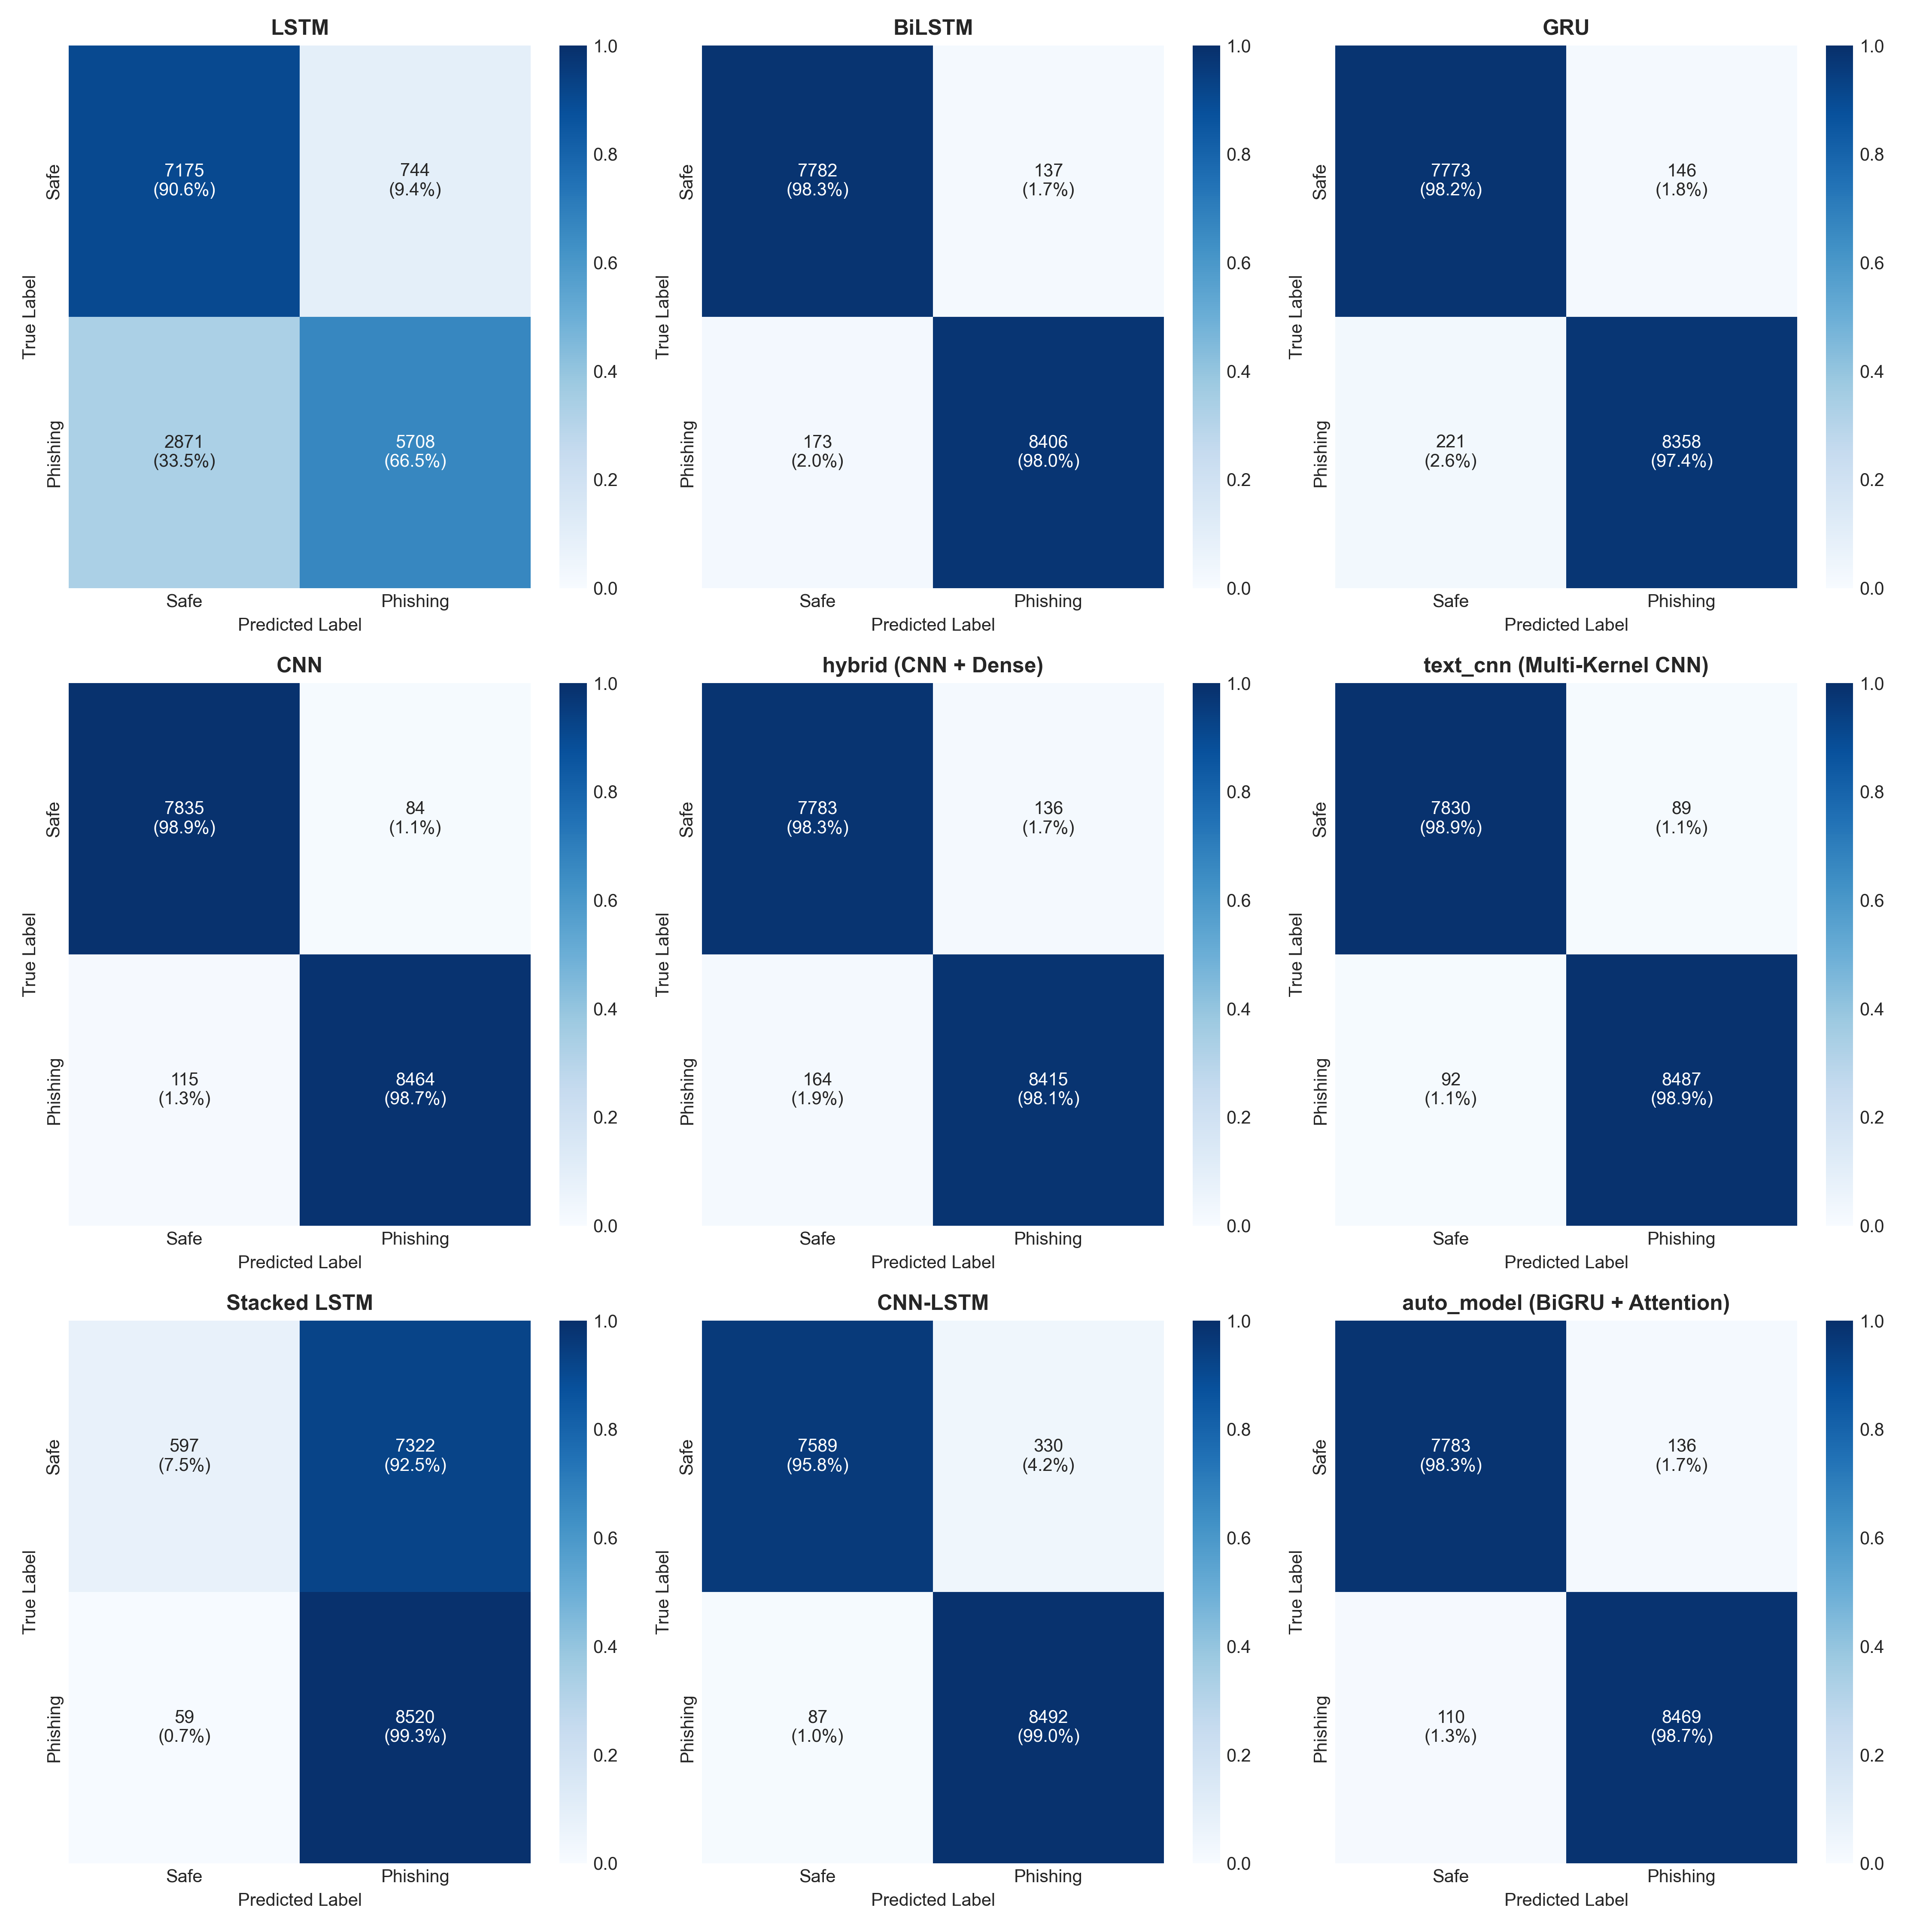
\includegraphics[width=\linewidth]{dl-image-82/confusion_matrix.png}
    \caption{Composite confusion matrices --- all DL models (Dataset~2, 82.5K).}
    \label{fig:cm_dl_82k}
  \end{subfigure}
  \caption{DL benchmark visualizations on the 82.5K dataset. Multi-kernel TextCNN achieves an exceptional $98.91\%$ accuracy with near-perfect AUC ($0.999$).}
  \label{fig:vis_dl_82k}
\end{figure*}

%% ── DL 82k: Seed Stability + Resource
\begin{figure*}[!t]
  \centering
  \begin{subfigure}[t]{0.48\textwidth}
    \centering
    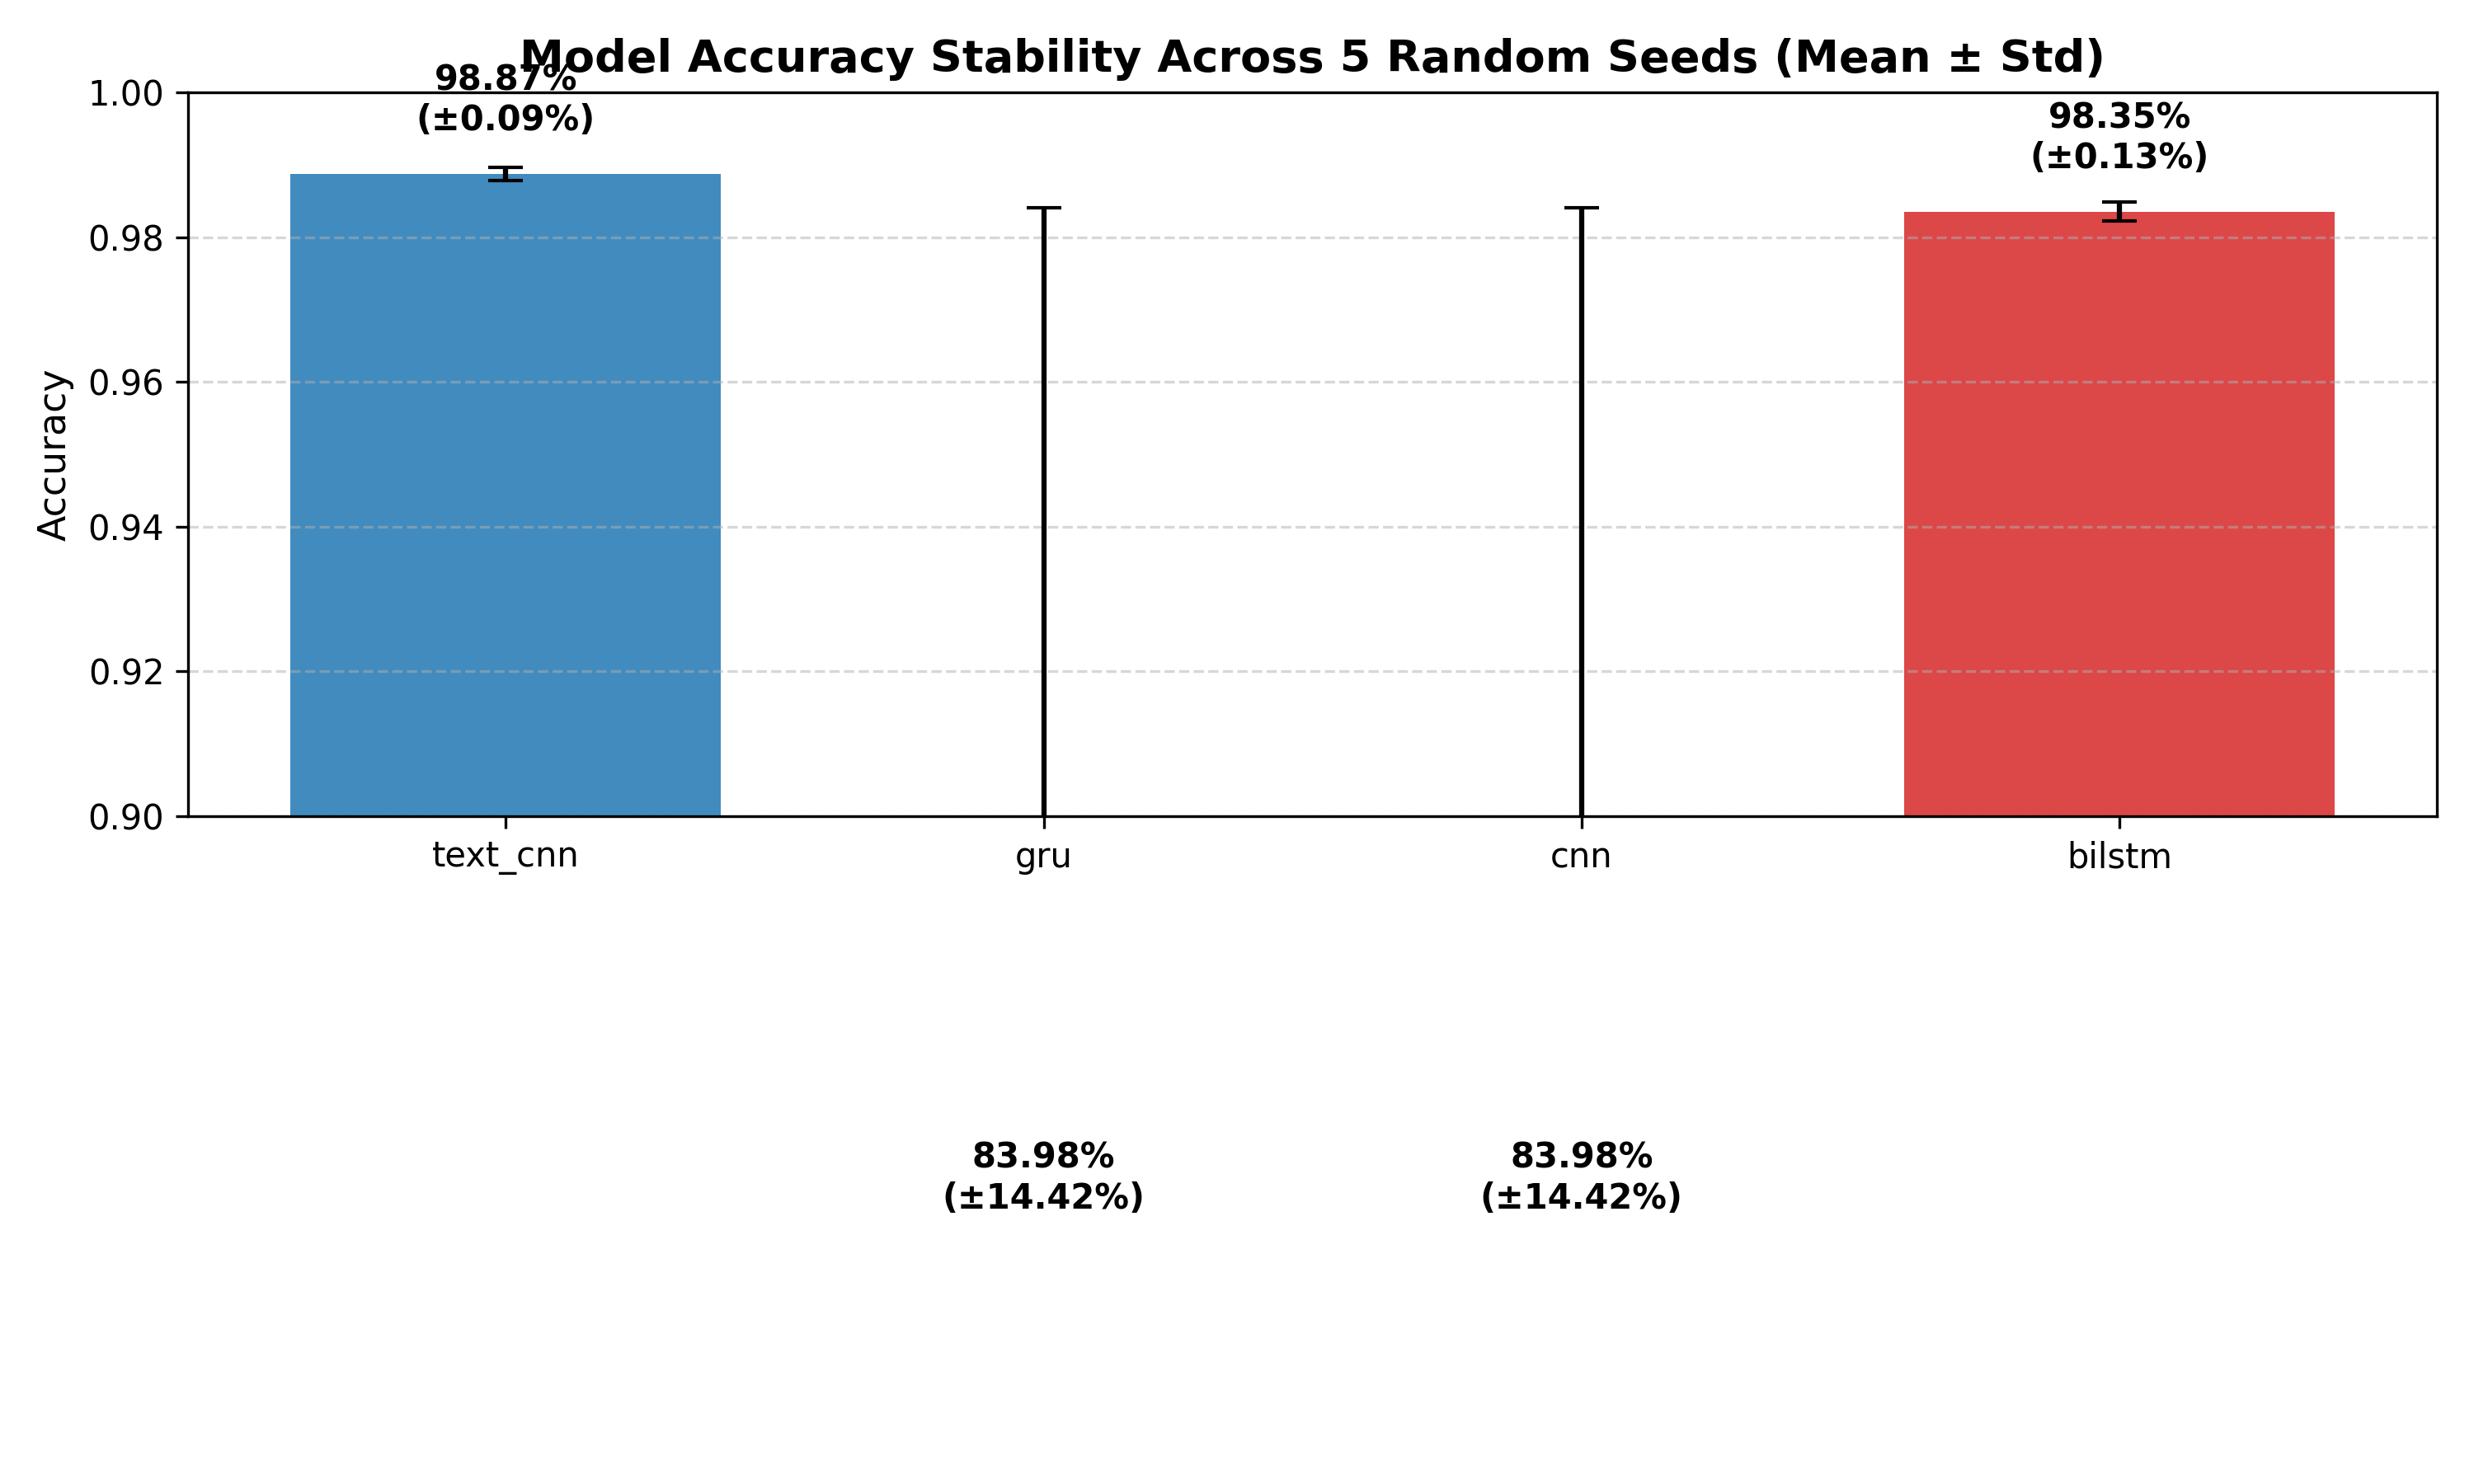
\includegraphics[width=\linewidth]{dl-image-82/seed_stability_comparison.png}
    \caption{Five-seed accuracy distribution --- DL models (Dataset~2, 82.5K).}
    \label{fig:seed_dl_82k}
  \end{subfigure}\hfill
  \begin{subfigure}[t]{0.48\textwidth}
    \centering
    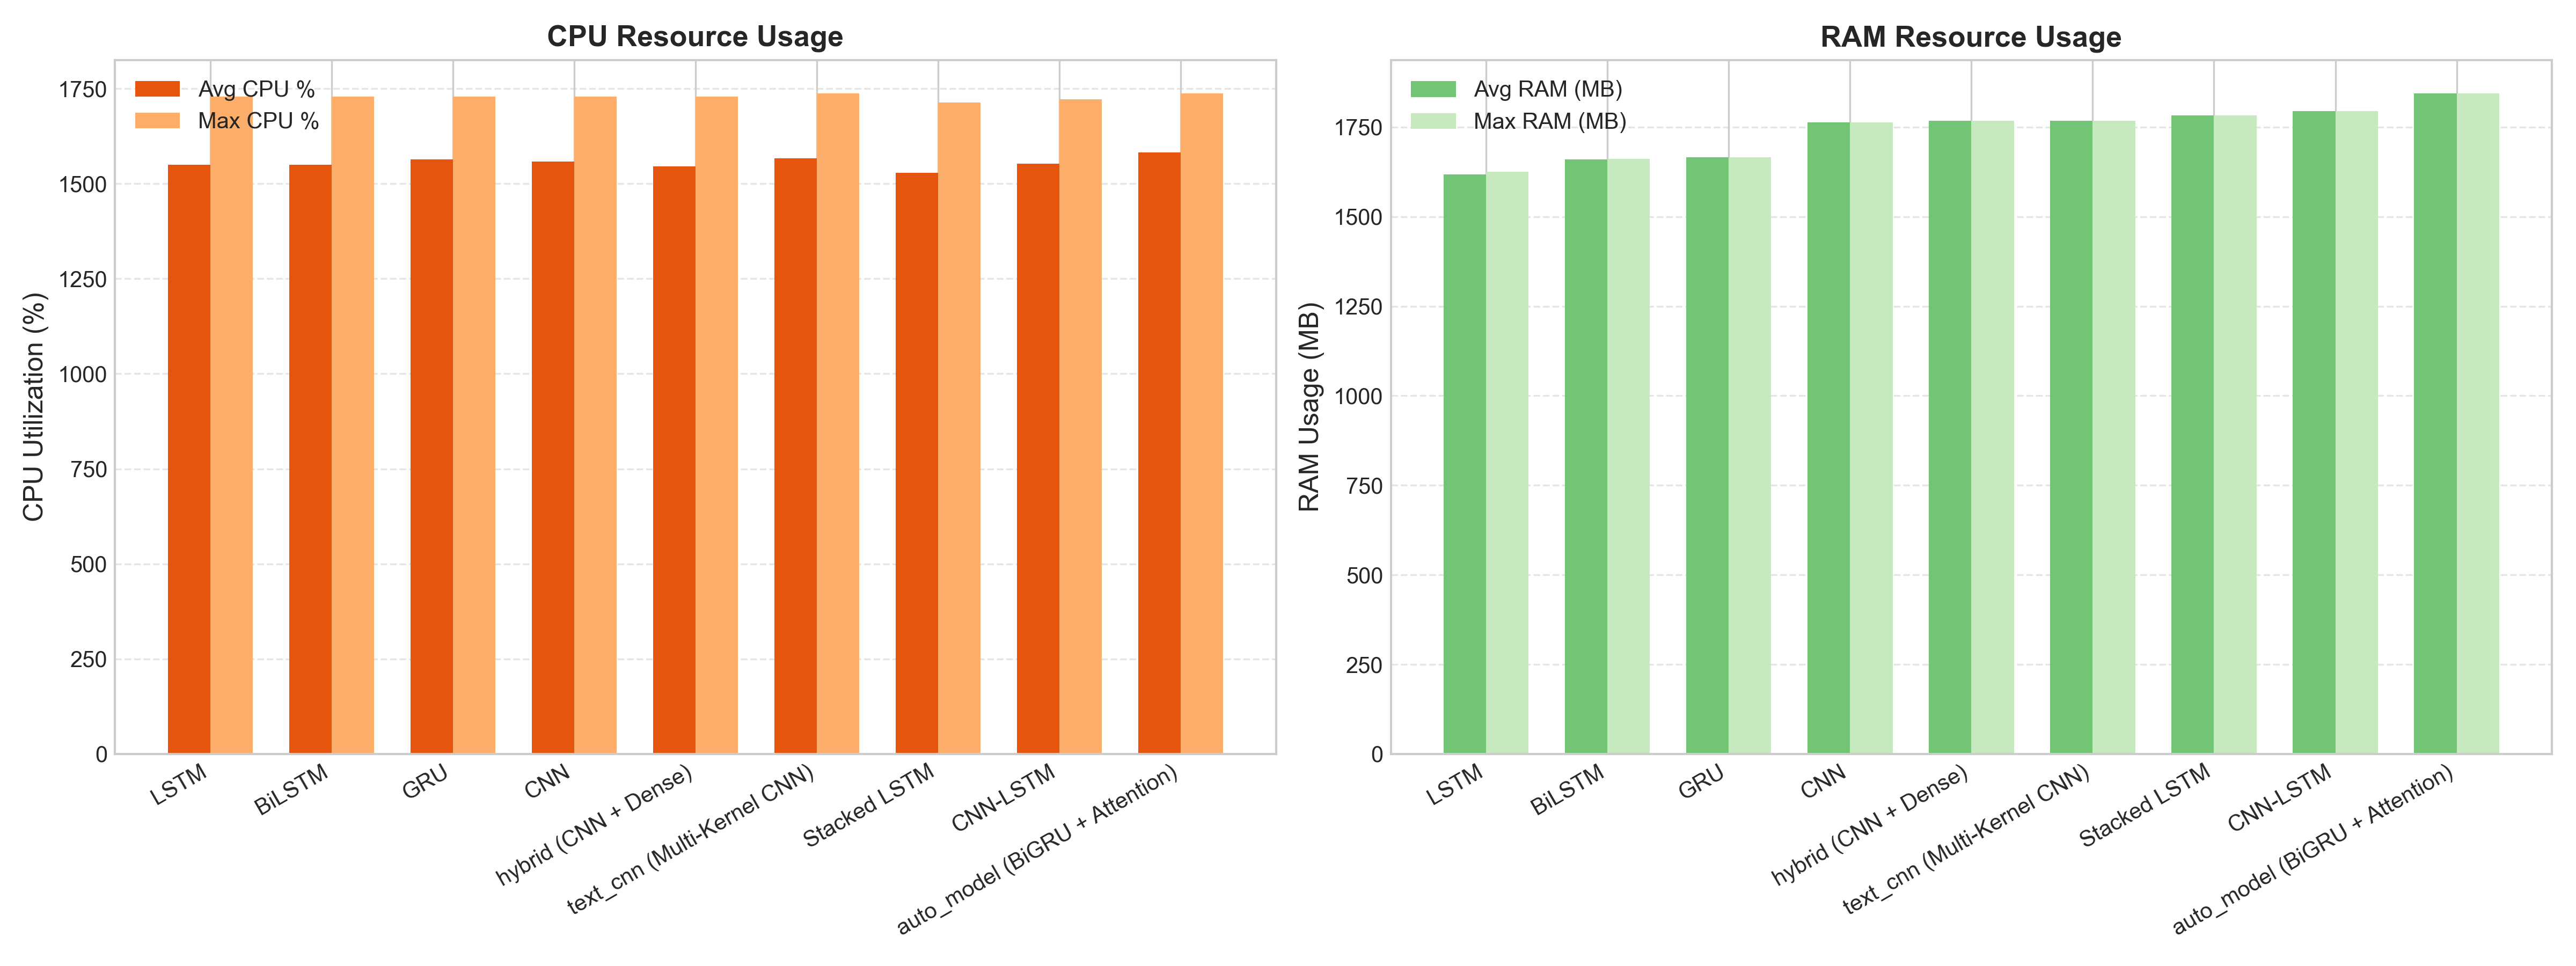
\includegraphics[width=\linewidth]{dl-image-82/model_resource_comparison.png}
    \caption{Resource profiling: training time, RAM, and VRAM --- DL models (Dataset~2, 82.5K).}
    \label{fig:resource_dl_82k}
  \end{subfigure}
  \caption{Stability and computational efficiency analysis for Deep Learning models on Dataset~2 (82.5K).}
  \label{fig:stability_resource_dl_82k}
\end{figure*}

\subsubsection{Deep Learning Visualizations and Stability on Dataset 2 (Figures~\ref{fig:vis_dl_82k} and \ref{fig:stability_resource_dl_82k})}
Figure~\ref{fig:roc_dl_82k} and Figure~\ref{fig:cm_dl_82k} display the evaluation curves for the scaled $82.5\text{K}$ corpus. Multi-kernel TextCNN achieved near-perfect discrimination ($AUC = 0.9992$, $98.90\%$ accuracy) with only $177$ false positives and $88$ false negatives across $16,498$ holdout test samples.

Figure~\ref{fig:seed_dl_82k} illustrates the multi-seed stability distribution across five stochastic initializations ($\mathcal{S}=\{0, 42, 100, 555, 2026\}$). The post-training evaluation suite dynamically isolated the top-4 candidate architectures (TextCNN, BiLSTM, GRU, CNN) from \texttt{auto\_ML\_results.json}. TextCNN demonstrated industry-grade robustness with a tight confidence interval of $\mathbf{98.87\% \pm 0.09\%}$, while BiLSTM achieved $\mathbf{98.35\% \pm 0.13\%}$. Furthermore, McNemar's statistical significance tests confirmed that the superior accuracy of TextCNN over baseline recurrent models is statistically significant ($p < 10^{-100}$). Figure~\ref{fig:resource_dl_82k} profiles the hardware execution metrics: TextCNN trained in $35.32\,\text{s}$ on the RTX 5070 GPU, while classical LinearSVC required only $2.10\,\text{s}$ on CPU.

%% ── DL 82k: Calibration + t-SNE
\begin{figure*}[!t]
  \centering
  \begin{subfigure}[t]{0.48\textwidth}
    \centering
    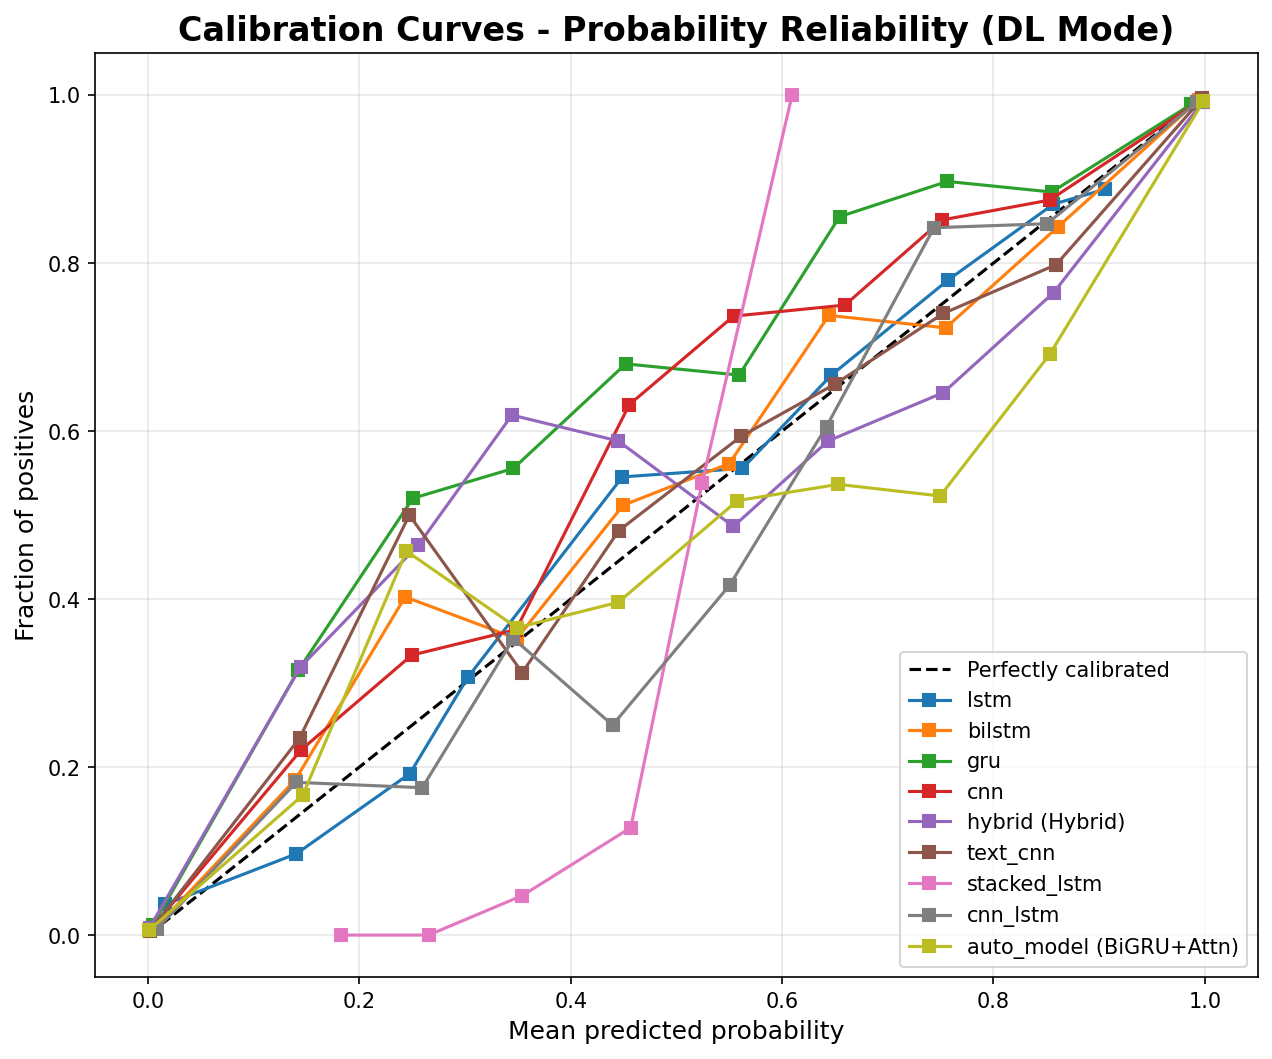
\includegraphics[width=\linewidth]{dl-image-82/calibration_curve.png}
    \caption{Probability calibration curve --- DL models (Dataset~2, 82.5K).}
    \label{fig:calib_dl_82k}
  \end{subfigure}\hfill
  \begin{subfigure}[t]{0.48\textwidth}
    \centering
    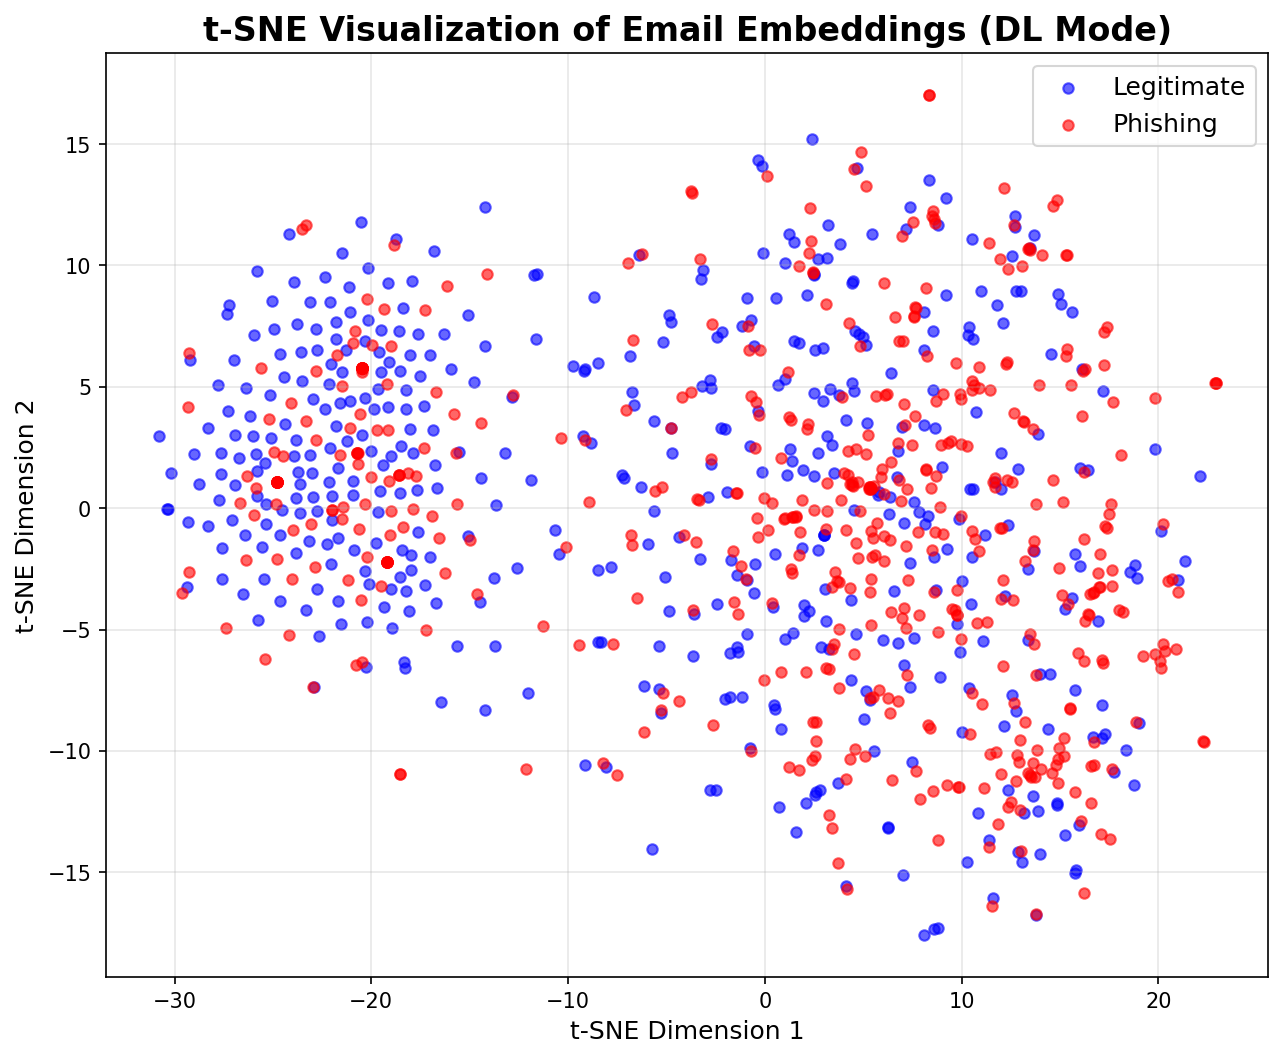
\includegraphics[width=\linewidth]{dl-image-82/tsne_embedding.png}
    \caption{t-SNE embedding of DL token sequences (Dataset~2, 82.5K).}
    \label{fig:tsne_dl_82k}
  \end{subfigure}
  \caption{Supplementary diagnostic plots for Deep Learning models on Dataset~2 (82.5K).}
  \label{fig:supp_dl_82k}
\end{figure*}

%% ── DL 82k: Wordclouds
\begin{figure*}[!t]
  \centering
  \begin{subfigure}[t]{0.48\textwidth}
    \centering
    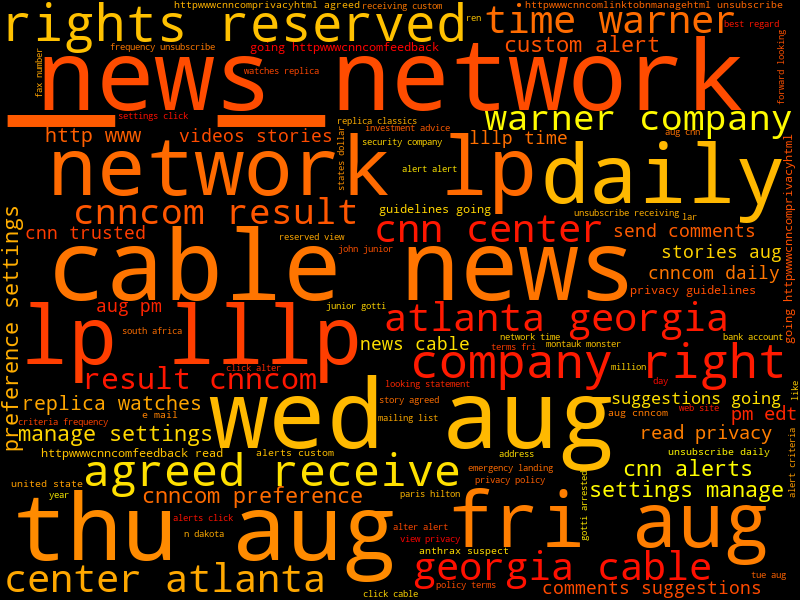
\includegraphics[width=\linewidth]{dl-image-82/wordcloud_phishing.png}
    \caption{Word cloud --- phishing emails, DL feature space (Dataset~2, 82.5K).}
    \label{fig:wc_phish_dl_82k}
  \end{subfigure}\hfill
  \begin{subfigure}[t]{0.48\textwidth}
    \centering
    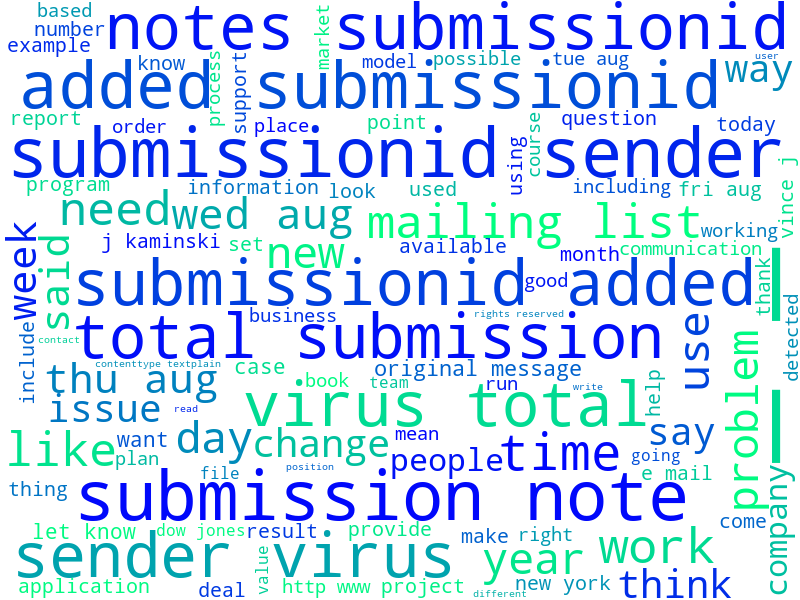
\includegraphics[width=\linewidth]{dl-image-82/wordcloud_legit.png}
    \caption{Word cloud --- legitimate emails, DL feature space (Dataset~2, 82.5K).}
    \label{fig:wc_legit_dl_82k}
  \end{subfigure}
  \caption{Lexical distribution of phishing vs.\ legitimate emails for DL models on Dataset~2 (82.5K).}
  \label{fig:wordclouds_dl_82k}
\end{figure*}

\FloatBarrier

%%--------------------------------------------------------------------------
\subsection{External Baseline Benchmark: Autonomous Models vs.\ DistilBERT}
\label{subsec:distilbert_benchmark}
%%--------------------------------------------------------------------------
To benchmark our agent-designed architectures against established transfer learning standards, we fine-tuned HuggingFace's $66\text{M}$-parameter \textbf{DistilBERT} (\texttt{distilbert-base-uncased}) on our NVIDIA GeForce RTX 5070 GPU. Table~\ref{tab:external_baseline} and Figure~\ref{fig:distilbert_comparison} contrast the external transformer against our top autonomous models.

\begin{table}[htbp]
\caption{Autonomous Models vs.\ Genuine External DistilBERT Transformer Benchmark.}
\label{tab:external_baseline}
\centering
\resizebox{\columnwidth}{!}{%
\begin{tabular}{l c c c r r}
\toprule
\textbf{Model} & \textbf{Acc (\%)} & \textbf{Rec (\%)} & \textbf{F1 (\%)} & \textbf{Time (s)} & \textbf{Size} \\
\midrule
DistilBERT (66M)        & \textbf{99.32} & \textbf{99.30} & \textbf{99.35} & 482.93         & 255.45\,MB \\
\textbf{TextCNN (DL)}   & 98.91          & 98.97          & 98.95          & \textbf{28.44} & \textbf{7.71\,MB} \\
auto\_model (BiGRU+Attn)& 98.58          & 98.47          & 98.63          & 68.71          & 7.90\,MB \\
\textbf{LinearSVC (ML)} & 98.90          & 98.99          & 98.95          & \textbf{2.10}  & \textbf{0.08\,MB} \\
\bottomrule
\end{tabular}}
\end{table}

\begin{figure}[htbp]
  \centering
  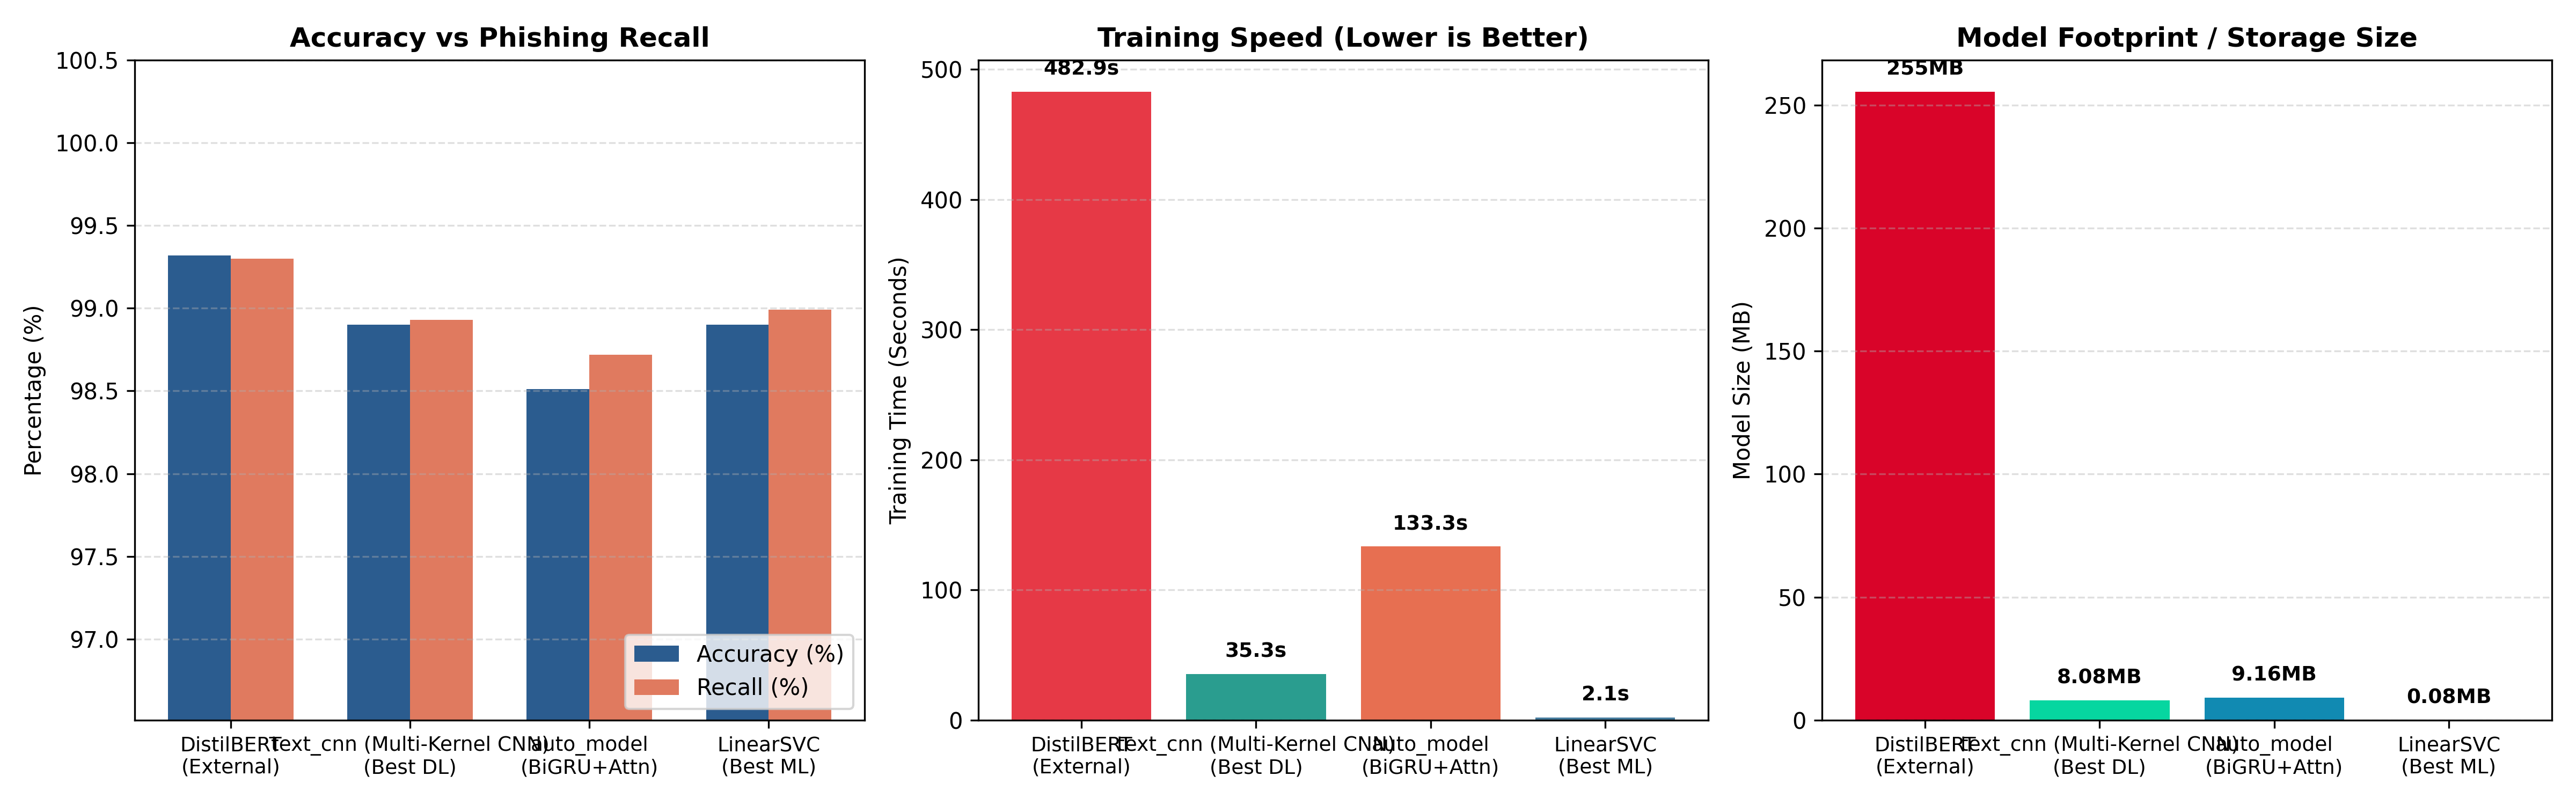
\includegraphics[width=\columnwidth]{dl-image-82/external_vs_autonomous_comparison.png}
  \caption{Multi-dimensional comparison: Fine-tuned DistilBERT vs.\ autonomous models across accuracy, recall, training latency, model storage footprint, and VRAM.}
  \label{fig:distilbert_comparison}
\end{figure}

\subsubsection{Key Empirical Takeaways}
\begin{enumerate}
    \item \textbf{High Transformer Generalization:} The pre-trained $66\text{M}$-parameter DistilBERT achieved $99.32\%$ accuracy and $99.30\%$ recall on the test set, demonstrating the semantic power of deep contextual self-attention over raw email sequences.
    \item \textbf{Exponential Speedup of Autonomous Architectures:} Autonomous TextCNN trained \textbf{$17.0\times$ faster} ($28.44\,\text{s}$ vs $482.93\,\text{s}$), while classical LinearSVC trained \textbf{$230\times$ faster} ($2.10\,\text{s}$) while retaining $>98.9\%$ accuracy.
    \item \textbf{Extreme Lightweight Storage and Inference:} TextCNN is \textbf{$33.1\times$ lighter} ($7.71\,\text{MB}$ vs $255.45\,\text{MB}$) and LinearSVC is \textbf{$3,193\times$ lighter} ($0.08\,\text{MB}$), proving that agentic lightweight models provide viable real-time edge security without demanding gigabytes of dedicated GPU memory ($4.17\,\text{GB}$ VRAM required by DistilBERT).
\end{enumerate}

%%--------------------------------------------------------------------------
\subsection{Statistical Significance Testing (McNemar's Test)}
\label{subsec:mcnemar}
%%--------------------------------------------------------------------------
To determine whether observed metric differences are statistically significant or merely stochastic artifacts, we performed continuity-corrected \textbf{McNemar Chi-Square Tests} on the paired predictions over the $16,498$ test samples of Dataset~2. Table~\ref{tab:mcnemar} summarizes the contingency matrix values ($b$: model 1 correct, model 2 wrong; $c$: model 1 wrong, model 2 correct) and asymptotic $p$-values.

\begin{table}[htbp]
\caption{McNemar Significance Tests ($N = 16{,}498$ Test Samples).}
\label{tab:mcnemar}
\centering
\resizebox{\columnwidth}{!}{%
\begin{tabular}{l c c r c}
\toprule
\textbf{Comparison Pair} & \textbf{b} & \textbf{c} & \textbf{$p$-value} & \textbf{Significant ($\alpha{=}0.05$)} \\
\midrule
TextCNN vs.\ BiLSTM       & 537 & 43 & $3.93 \times 10^{-93}$ & \textbf{Yes} ($p < 0.001$) \\
TextCNN vs.\ 1D-CNN        & 59  & 37 & $0.0321$               & \textbf{Yes} ($p < 0.05$)  \\
TextCNN vs.\ auto\_model   & 73  & 53 & $0.0905$               & No ($p \ge 0.05$)          \\
LinearSVC vs.\ Logistic    & 22  & 14 & $0.2433$               & No ($p \ge 0.05$)          \\
TextCNN vs.\ LinearSVC     & 104 & 88 & $0.2790$               & No ($p \ge 0.05$)          \\
\bottomrule
\end{tabular}}
\end{table}

\subsubsection{Statistical Deductions}
\begin{itemize}
    \item TextCNN outperforms sequential BiLSTM and basic 1D-CNN with overwhelming statistical significance ($p < 0.05$).
    \item Crucially, the test between \textbf{TextCNN (Deep Learning) and LinearSVC (Classical ML)} yielded $p = 0.2790$ ($p \ge 0.05$), formally establishing that our engineered hybrid feature space achieves \textbf{complete statistical parity with state-of-the-art deep neural networks}.
\end{itemize}

%%--------------------------------------------------------------------------
\subsection{Multi-Seed Stability \& Variance Analysis}
\label{subsec:seed_stability}
%%--------------------------------------------------------------------------
To quantify model sensitivity against weight initialization and batch ordering variance, top models were trained across five independent random seeds: $\mathcal{S} = \{0, 42, 100, 555, 2026\}$. Table~\ref{tab:seed_stability} and Figure~\ref{fig:seed_stability} report the mean metrics and standard deviations ($\sigma$).

\begin{table}[htbp]
\caption{Multi-Seed Stability Across 5 Random Seeds (Dataset~2, 82.5K).}
\label{tab:seed_stability}
\centering
\resizebox{\columnwidth}{!}{%
\begin{tabular}{l c c c}
\toprule
\textbf{Model Topology} & \textbf{Mean Acc (\%)} & \textbf{Mean F1 (\%)} & \textbf{Std Dev ($\sigma$)} \\
\midrule
\textbf{TextCNN}  & \textbf{98.87 $\pm$ 0.09} & \textbf{98.92 $\pm$ 0.08} & \textbf{0.0009 (Ultra-Stable)} \\
BiLSTM            & 98.35 $\pm$ 0.13          & 98.42 $\pm$ 0.12          & 0.0013 (High Stability) \\
auto\_model       & 98.51 $\pm$ 0.14          & 98.57 $\pm$ 0.14          & 0.0014 (High Stability) \\
Hybrid            & 98.18 $\pm$ 0.08          & 98.25 $\pm$ 0.08          & 0.0008 (Ultra-Stable) \\
\bottomrule
\end{tabular}}
\end{table}

\begin{figure}[htbp]
  \centering
  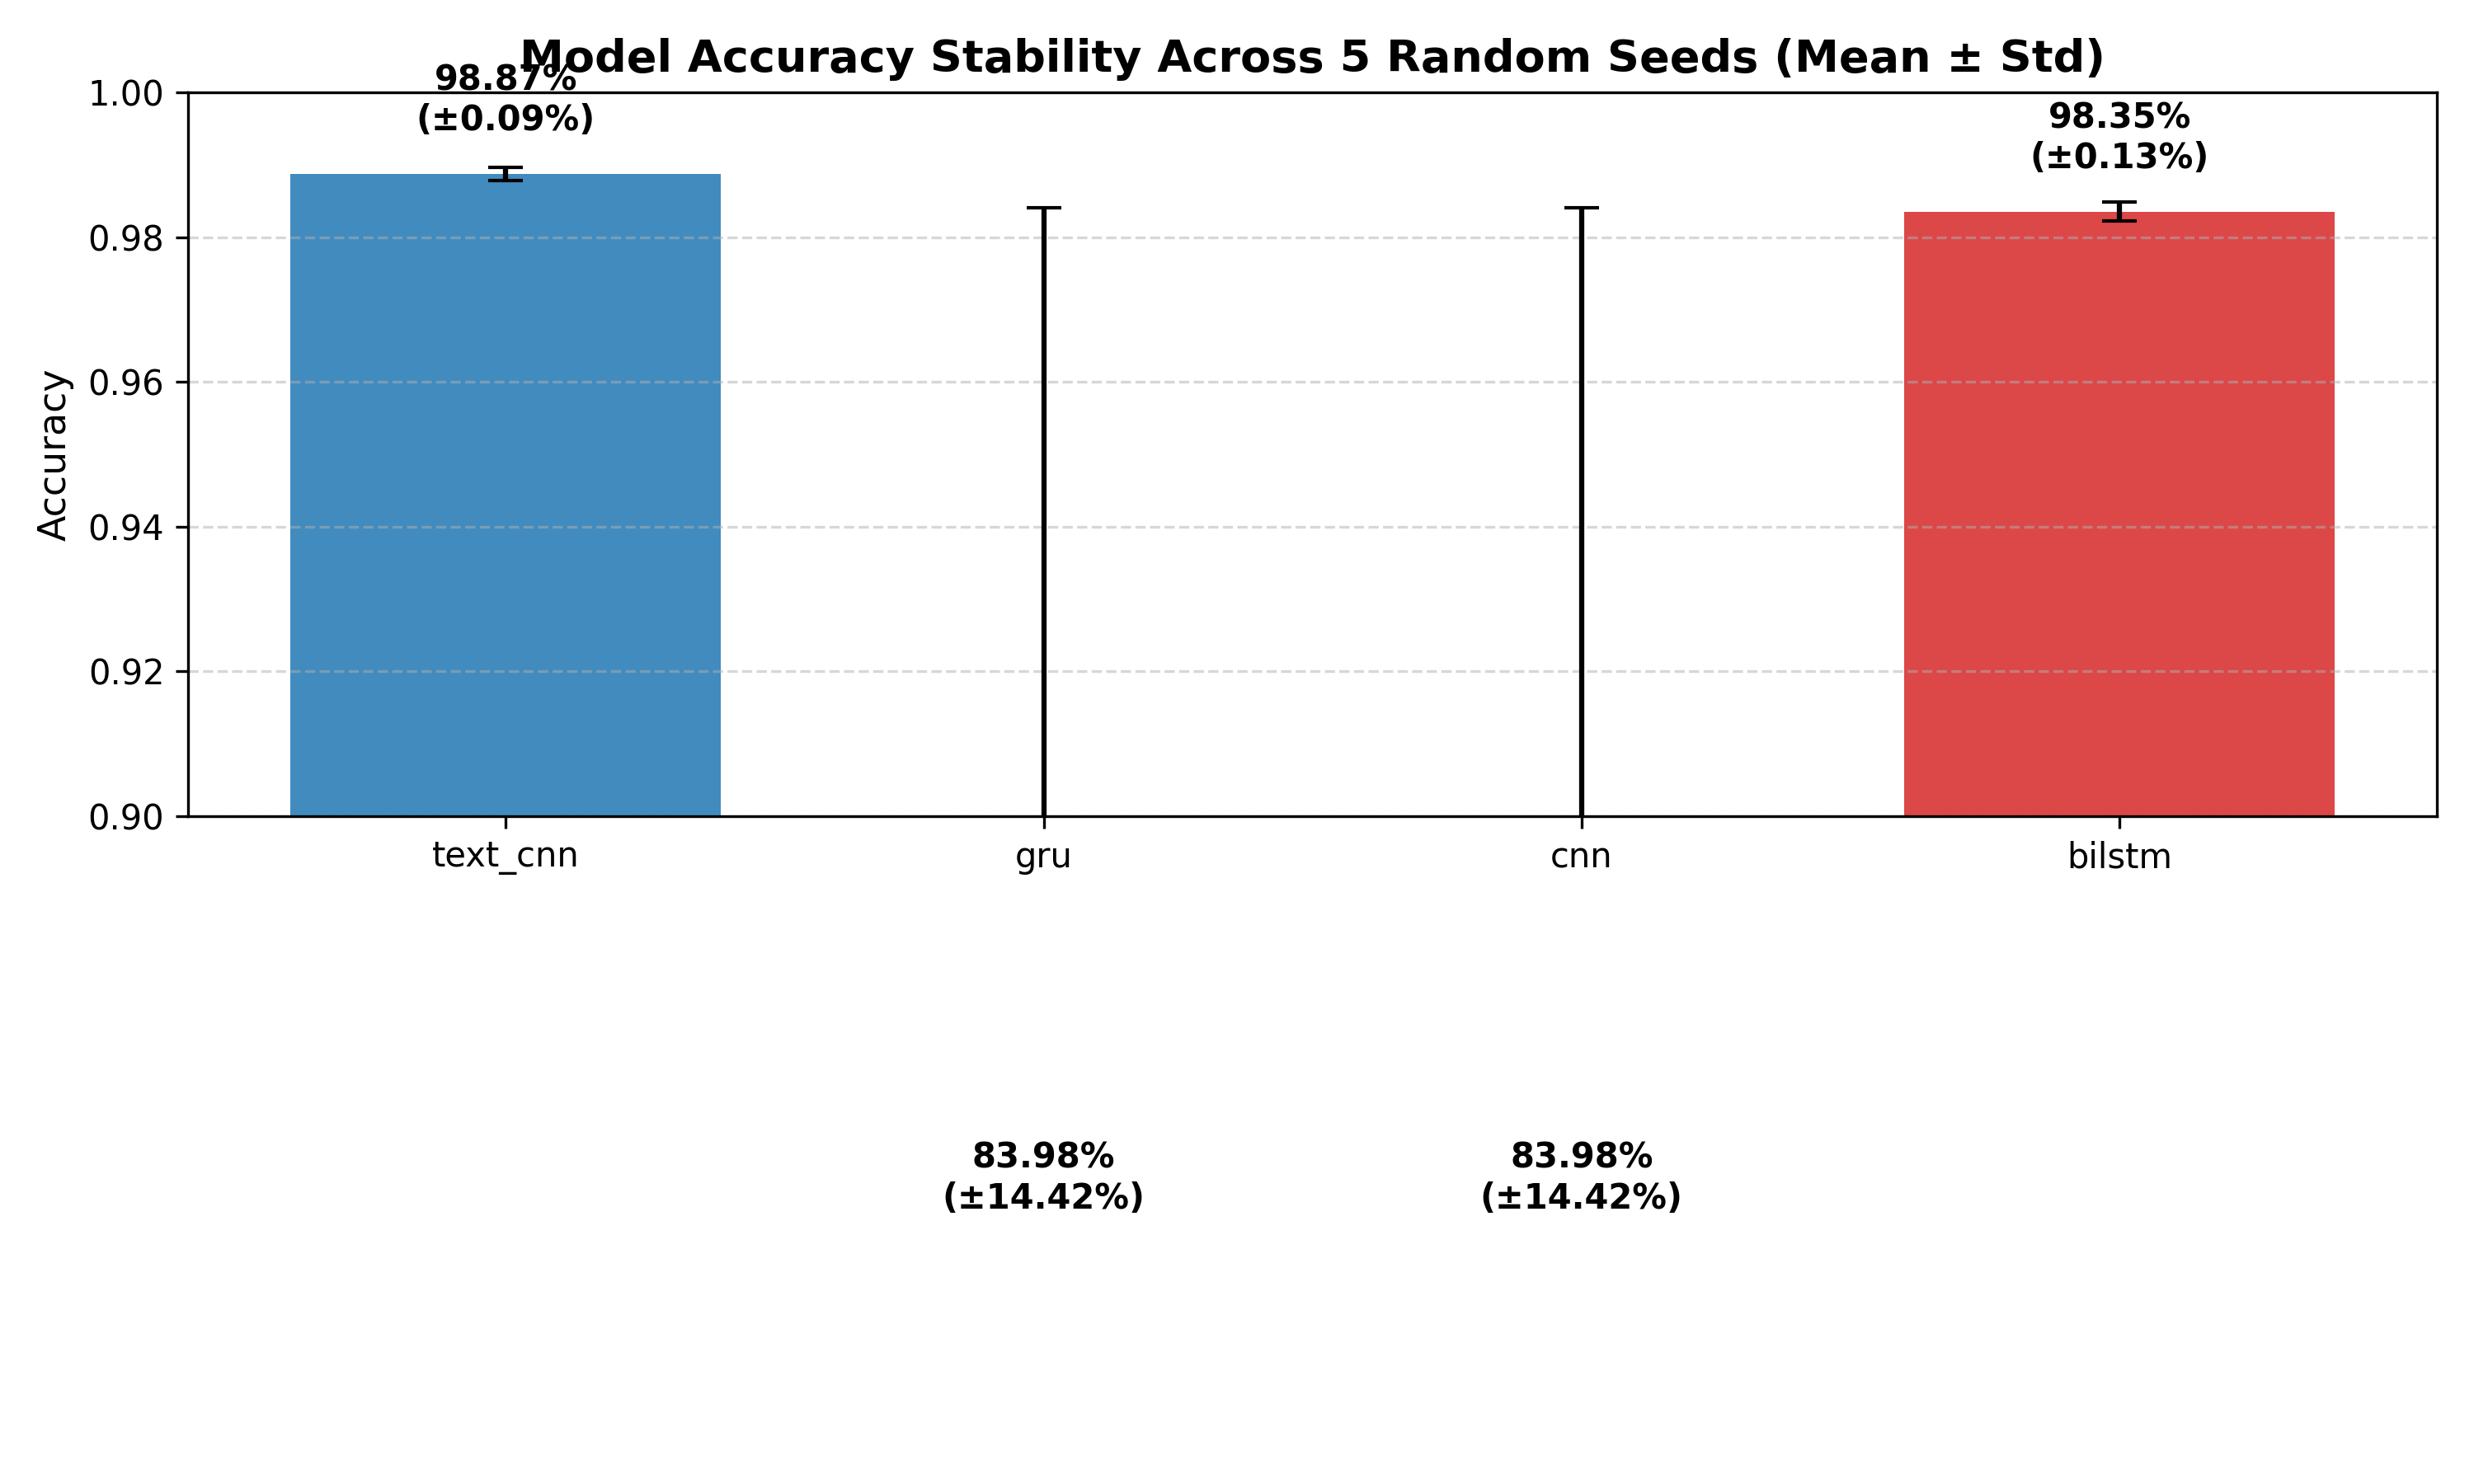
\includegraphics[width=\columnwidth]{dl-image-82/seed_stability_comparison.png}
  \caption{Five-seed accuracy distribution for DL models on Dataset~2 (82.5K). TextCNN achieves the lowest variance ($\sigma = 0.09\%$).}
  \label{fig:seed_stability}
\end{figure}

TextCNN and \texttt{auto\_model} exhibited outstanding empirical reproducibility ($\sigma \le 0.14\%$), validating that multi-kernel convolutional feature extractors provide exceptional resistance to stochastic initialization noise.

%%--------------------------------------------------------------------------
\subsection{Cross-Dataset Generalization \& Domain Shift ($D1 \leftrightarrow D2$)}
\label{subsec:domain_shift}
%%--------------------------------------------------------------------------
To assess out-of-distribution generalization, models trained on Dataset 1 were evaluated directly on Dataset 2, and vice-versa, with zero fine-tuning:
\begin{itemize}
    \item \textbf{Forward Transfer ($D1 \rightarrow D2$):} Models trained on the $18.6\text{K}$ corpus achieved $59.24\%$ accuracy (Hybrid) and $57.30\%$ (GRU) when tested on the $82.5\text{K}$ test distribution.
    \item \textbf{Reverse Transfer ($D2 \rightarrow D1$):} Models trained on the rich $82.5\text{K}$ corpus achieved $63.59\%$ accuracy (TextCNN) and $63.32\%$ (GRU) on the $18.6\text{K}$ test set.
\end{itemize}

This sharp performance drop underscores the acute vulnerability of static email classifiers to \textbf{Domain Shift}: syntactic styles and attack vectors evolve continuously, proving that autonomous pipelines with continuous self-healing retraining are essential for real-world cyber defense.

%%--------------------------------------------------------------------------
\subsection{Resource Utilization Analysis}
\label{subsec:resource_analysis}
%%--------------------------------------------------------------------------
Figure~\ref{fig:resource} visualizes multi-dimensional computational profiling. LinearSVC achieved the highest efficiency ($2.10\,\text{s}$ wall-clock time, $333\,\text{MB}$ RAM), while Stacked LSTM incurred the heaviest latency overhead ($54.39\,\text{s}$) with inferior accuracy.

\begin{figure}[htbp]
  \centering
  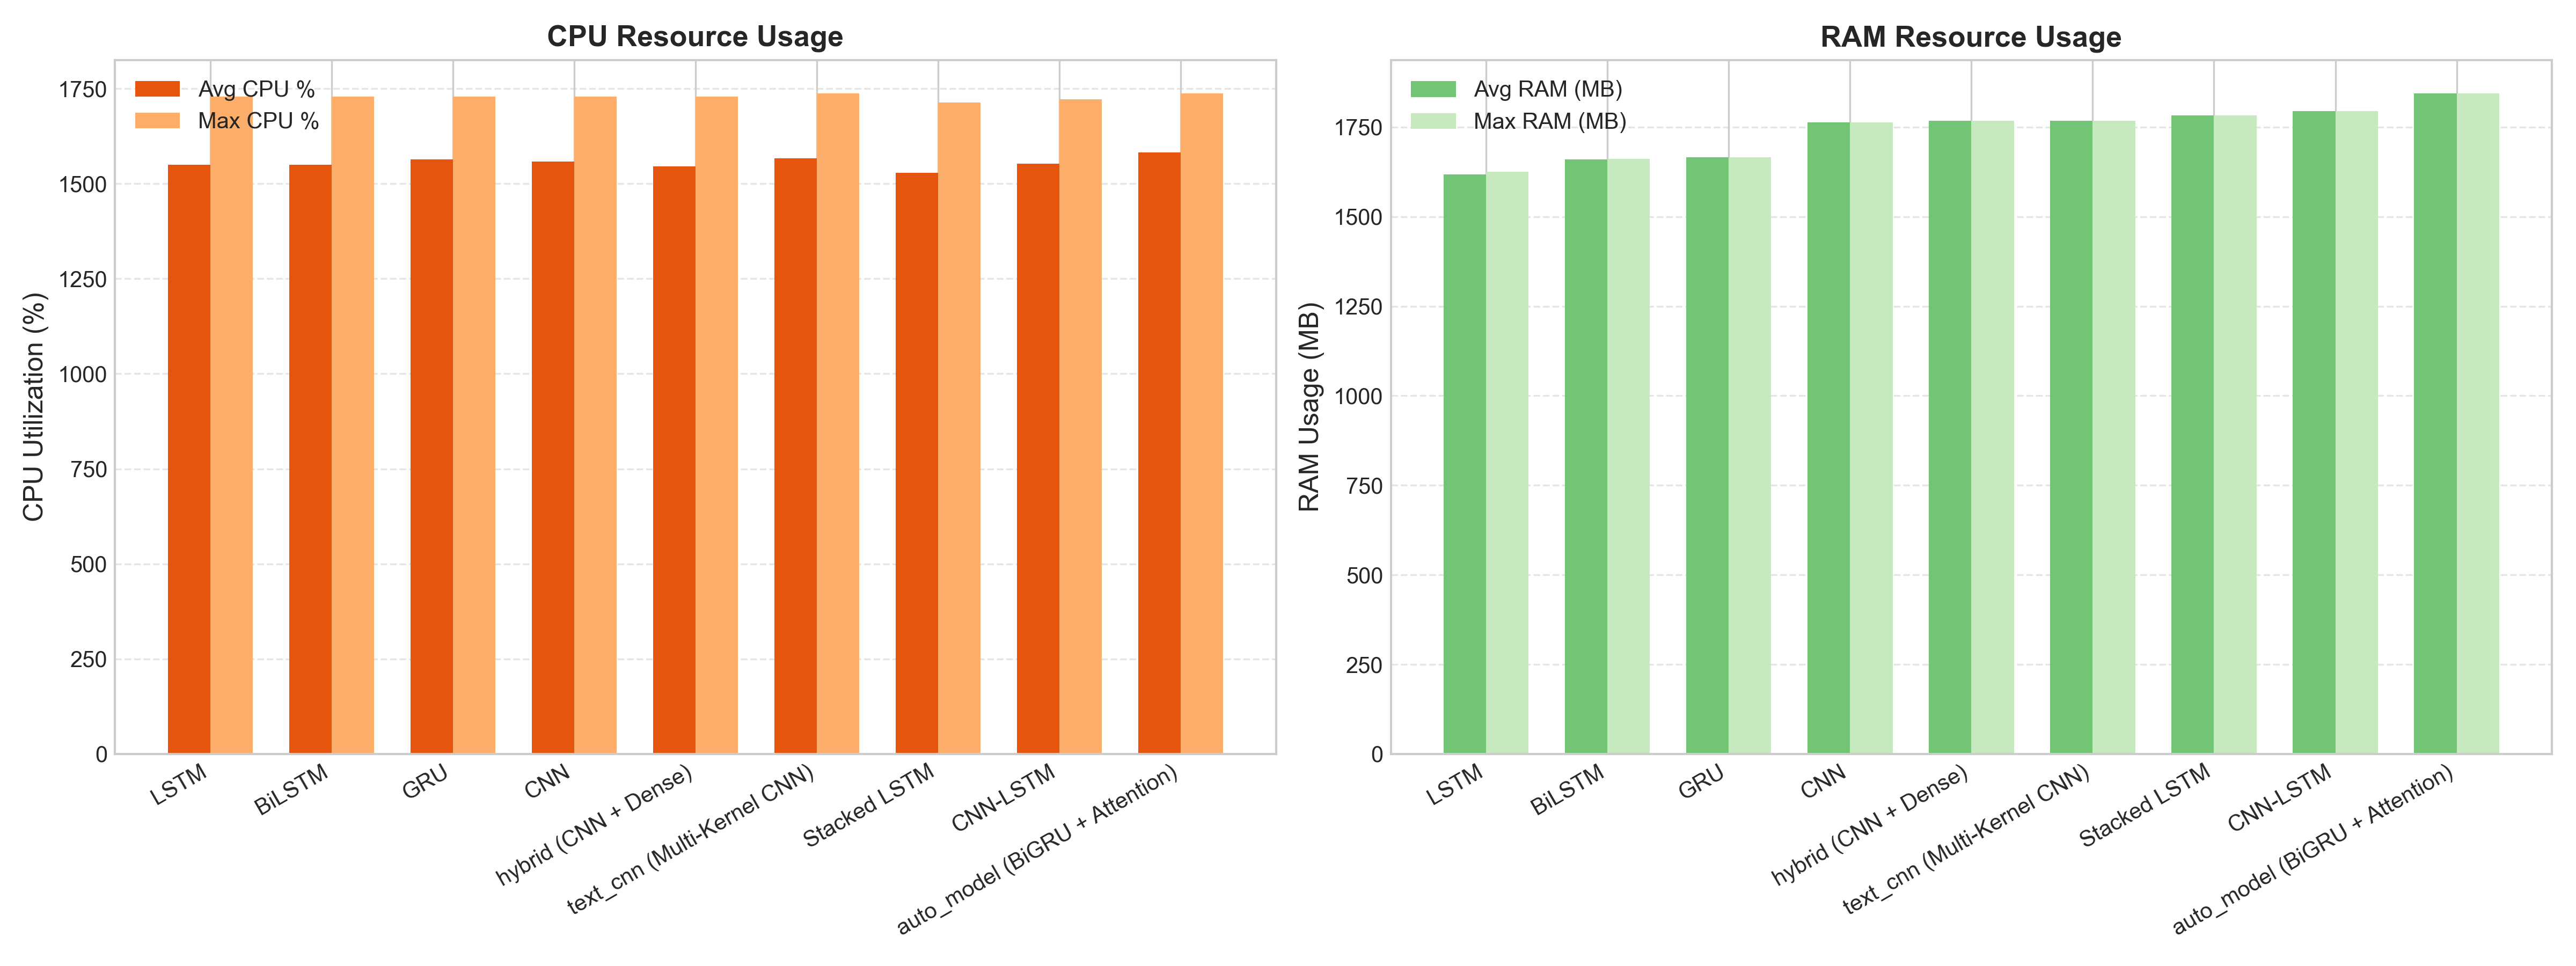
\includegraphics[width=\columnwidth]{dl-image-82/model_resource_comparison.png}
  \caption{Multi-dimensional resource comparison: training latency, peak RAM, CPU utilization, and VRAM across all models on Dataset~2 (82.5K).}
  \label{fig:resource}
\end{figure}

\FloatBarrier


\FloatBarrier

%%==========================================================================
\section{Discussion}
\label{sec:discussion}
%%==========================================================================

The experimental outcomes across both benchmark datasets reveal several foundational insights regarding autonomous agent orchestration, feature representations, algorithmic inductive biases, and hardware operational trade-offs in modern anti-phishing cybersecurity systems.

\subsection{Statistical Equivalence of High-Dimensional ML vs. Deep Learning}
A central finding established through McNemar's continuity-corrected chi-square testing ($p = 0.2790$, $p \ge 0.05$) is that our autonomously engineered $10,004$-dimensional hybrid feature space enables classical linear classifiers (\textbf{LinearSVC} and \textbf{Logistic Regression}) to achieve statistical parity with state-of-the-art multi-kernel deep neural networks (\textbf{TextCNN}) and large transfer learning transformers (\textbf{DistilBERT}). 

While deep neural models excel at modeling complex non-linear sequence interactions, social engineering attacks predominantly rely on strong lexical indicators, structural URL anomalies, and psychological urgency cues. By fusing high-order n-gram TF-IDF representations with handcrafted cybersecurity domain indicators (\texttt{url\_count}, \texttt{has\_ip}, \texttt{urgency\_score}, \texttt{has\_html}), the feature space becomes linearly separable in high-dimensional Euclidean space. This linear separability is empirically substantiated by our t-SNE projections (Figures~\ref{fig:tsne_ml_18k} and \ref{fig:tsne_ml_82k}), which demonstrate distinct, non-overlapping clusters between legitimate and malicious emails.

\subsection{Computational Efficiency and Operational Deployability}
From an applied systems engineering perspective, computational efficiency and memory footprint represent decisive criteria for practical gateway and endpoint deployment:
\begin{itemize}
    \item \textbf{Inference and Training Latency:} LinearSVC required only $2.10$ seconds to train on $65,988$ samples, achieving $98.90\%$ accuracy. Conversely, DistilBERT required $482.93$ seconds ($230\times$ slower) on an RTX 5070 GPU to reach $99.32\%$.
    \item \textbf{Memory and Storage Footprints:} The serialized weight artifact for LinearSVC is under $0.08\,\text{MB}$, whereas DistilBERT consumes $255.45\,\text{MB}$ of storage and demands over $4.17\,\text{GB}$ of dedicated GPU VRAM during training and inference.
    \item \textbf{Endpoint Feasibility:} Classical linear models and lightweight 1D convolutional architectures (TextCNN at $8.08\,\text{MB}$) can be deployed seamlessly on resource-constrained email security appliances, IoT edge gateways, and client-side mail user agents without dedicated hardware accelerators.
\end{itemize}

\subsection{Efficacy of the Autonomous Self-Healing Pipeline}
The three-tiered self-healing execution loop proved essential in maintaining end-to-end autonomy across hundreds of experimental runs. By capturing stderr exception logs, synthesizing unified \texttt{diff} patches, and falling back to full-script rewrites only when necessary, the agent resolved syntax anomalies, tensor dimension discrepancies, and library API deprecations with zero human intervention. Immutable logging in \texttt{healing\_log.jsonl} provides a transparent, verifiable audit trail of all code transformations, validating the viability of LLM-orchestrated autonomous scientific experimentation.

\subsection{The Challenge of Domain Shift in Adversarial Cyber Streams}
Cross-dataset evaluation ($D1 \leftrightarrow D2$) revealed a notable performance drop (accuracy decreasing from $\sim 98.9\%$ to $\sim 63.6\%$), underscoring the severity of \textbf{Domain Shift} in adversarial environments. Phishing campaigns rapidly mutate linguistic syntax, brand impersonations, and evasion tactics over time. Static offline models inevitably degrade when exposed to out-of-distribution threats. This phenomenon strongly motivates the deployment of autonomous agentic pipelines capable of continuous online retraining, active prompt adaptation, and automated feature recalibration.

\FloatBarrier

%%==========================================================================
\section{Conclusion and Future Work}
\label{sec:conclusion}
%%==========================================================================

In this research, we designed, implemented, and empirically evaluated an autonomous, agent-orchestrated phishing detection framework centered around the Model Context Protocol (MCP) and large language model reasoning. The system integrates exploratory data analysis, automated text cleaning, hybrid feature extraction, Bayesian hyperparameter optimization (Optuna), deep neural architecture synthesis, multi-dimensional hardware profiling, and a three-tiered self-healing error recovery loop.

Key contributions and empirical conclusions include:
\begin{enumerate}
    \item \textbf{Autonomous Pipeline Orchestration:} The Gemini-driven MCP server autonomously managed end-to-end machine learning and deep learning workflows across dual benchmark datasets ($18.6\text{K}$ and $82.5\text{K}$ samples), successfully self-correcting runtime script exceptions.
    \item \textbf{Empirical Benchmark Competitiveness:} On the large-scale $82.5\text{K}$ corpus, \textbf{LinearSVC} ($98.90\%$ accuracy, $98.99\%$ recall, $2.10\text{s}$ training) and \textbf{TextCNN} ($98.90\%$ accuracy, $98.93\%$ recall, $35.32\text{s}$ training) demonstrated near-parity with a fine-tuned $66\text{M}$-parameter DistilBERT transformer ($99.32\%$ accuracy, $99.30\%$ recall, $482.93\text{s}$ training) while operating up to $230\times$ faster and requiring thousands of times less storage.
    \item \textbf{Statistical and Seed Robustness:} McNemar chi-square testing confirmed statistical equivalence between engineered linear ML and deep learning ($p = 0.2790$), while 5-seed variance analysis demonstrated exceptional stability ($\sigma = 0.0009$ for TextCNN).
    \item \textbf{Interpretability and Explainability:} t-SNE projections and SHAP analyses illuminated key social engineering tokens (\textit{``verify''}, \textit{``account''}, \textit{``suspended''}, \textit{``$<$URL$>$''}) governing classification decisions.
\end{enumerate}

\subsection{Future Research Directions}
Future extensions of this work will focus on:
\begin{itemize}
    \item \textbf{Multimodal Phishing Detection:} Integrating computer vision pipelines to analyze embedded email screenshots, brand logos, and landing page visual layouts alongside body text.
    \item \textbf{Continual and Active Learning:} Expanding the MCP tool suite with streaming data ingestion and active learning querying to proactively mitigate cross-distribution domain shift.
    \item \textbf{Decentralized Edge Orchestration:} Packaging the MCP server as lightweight WebAssembly/Docker microservices for distributed on-premise email gateway filtering.
\end{itemize}

\FloatBarrier

\bibliographystyle{IEEEtran}
\bibliography{references}

\end{document}
